\documentclass[twoside]{article}
\setlength{\parindent}{0pt}

\usepackage{graphicx} % Required for inserting images
\usepackage[parfill]{parskip}
%\title{}
%\author{}
%\date{}
\usepackage{lineno}
\usepackage{hyperref}
\usepackage{booktabs}
\linenumbers
\usepackage{fancyhdr}
\usepackage{amsmath}
\usepackage{multirow}
\usepackage{float}
\usepackage{tikz}
%\usepackage{subcaption}
\usepackage{geometry}
%\usepackage{placeins}
\usepackage{caption}

\geometry{
 a4paper,
 left=30mm,
 right=30mm,
 top=50mm,
 bottom=30mm
 }


\begin{document}

\newcounter{rowcounter}
\pagestyle{fancy}
\fancyhf{}
\fancyhead[LE]{\nouppercase{\rightmark\hfill\leftmark}}
\fancyhead[RO]{\nouppercase{\leftmark\hfill\rightmark}}
\fancyfoot[LE,RO]{\hfill\thepage\hfill}

%\maketitle

\section{Introduction}
Four-top quark production ($t\bar{t}t\bar{t}$) is a rare process within the Standard Model (SM) that serves as a crucial probe for both SM and beyond-the-Standard-Model (BSM) physics. Figure \ref{fig:ftop_feymann} illustrates representative leading-order Feynman diagrams for $t\bar{t}t\bar{t}$ production. The latest predicted SM cross section for $t\bar{t}t\bar{t}$ production at next-to-leading order (NLO) with next-to-leading logarithmic (NLL') correction is 13.37 fb at $\sqrt{s}$ = 13 TeV and 15.82 TeV at $\sqrt{s}$ = 13.6 fb \cite{ftop_xsec}. This process is sensitive to the top quark's Yukawa coupling with the Higgs boson while remaining unaffected by the Higgs boson decay, making it a prime candidate for identifying any deviations from SM predictions regarding the top quark Yukawa coupling. Furthermore, deviations in the four-top production cross section from SM predictions could also signal the presence of undiscovered heavy scalar or pseudo-scalar bosons decaying into top quarks, as proposed in several extensions of the SM, including top-philic resonances as shown by Figure \ref{fig:tp_feymann}.\\

\begin{figure}[h!]
    \centering
    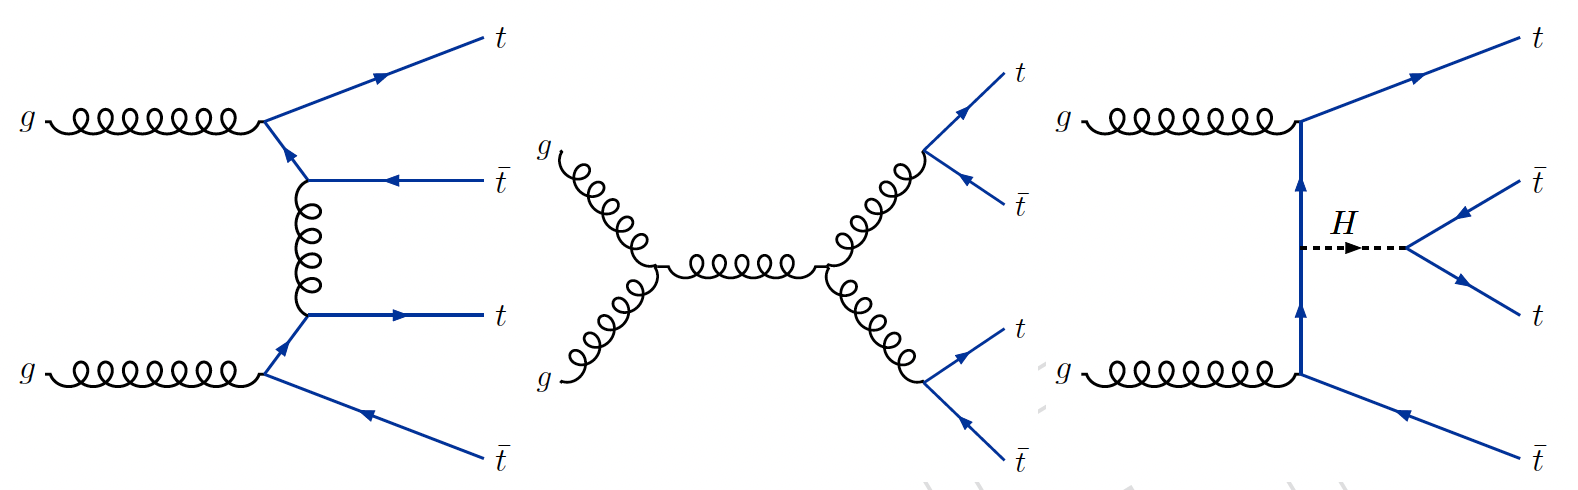
\includegraphics[width=0.8\textwidth]{plots/ftop_feymann.png}
    \caption{Representative LO Feynman diagrams for SM $t\bar{t}t\bar{t}$ production.}
    \label{fig:ftop_feymann}
\end{figure}

\begin{figure}[h!]
    \centering
    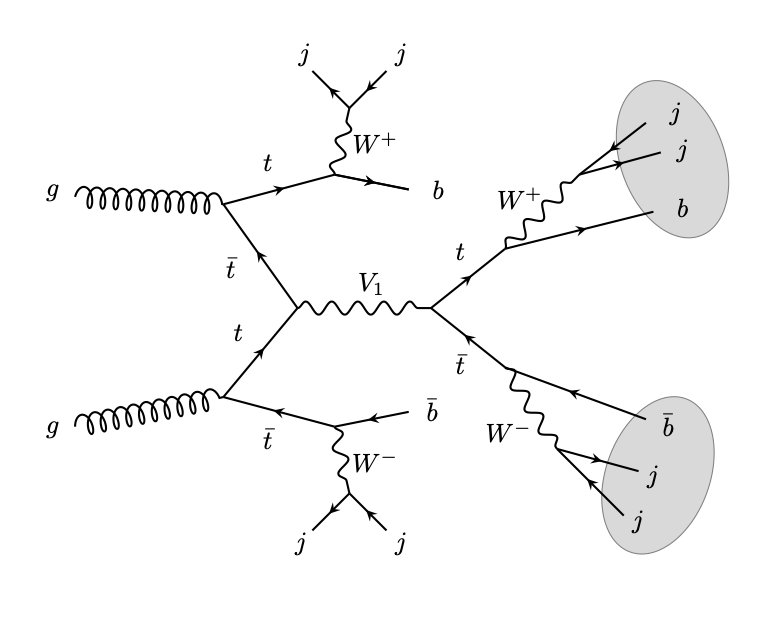
\includegraphics[width=0.8\textwidth]{plots/tp_feymann.png}
    \caption{Representative LO Feynman diagrams for tree-level single production of the V1 decaying into the fully-hadronic channel in the BSM top-philic resonance model.}
    \label{fig:tp_feymann}
\end{figure}

Each top quark predominantly decays into a bottom quark and a W boson. The W boson then decays either hadronically, producing quarks, or leptonically, yielding a lepton and a neutrino. In this analysis, the fully hadronic final state, where all four top quarks decay entirely into hadrons, is being investigated for the first time, representing about 20\% of all four-top quark events.\\

This analysis follows a previous CMS analysis on all-hadronic four-top production with Run2 dataset described in AN2020\_021. The observed significance of the \(t\bar{t}t\bar{t}\) signal in this channel was 2.5 standard deviations (with 0.4 expected). When combined \cite{prev_ftop_analysis} with other channels (Single Lepton, opposite-sign dilepton), the observed significance of the \(t\bar{t}t\bar{t}\) signal was 3.9 standard deviations (with 1.5 expected). In this analysis, we improve upon the previous all-hadronic channel analysis and expand it to include 2022, 2023 data. We will also include an interpretation against the top-philic resonance BSM model\cite{topphilic}.\\

The search for four-top quark production in the fully hadronic final state faces significant challenges due to substantial backgrounds from top quark pair (\(t\bar{t}\)) and QCD multijet production. To address these challenges, specialized machine learning tools for hadronic top quark tagging are utilized. In the "boosted" regime, where top quarks have high transverse momentum (\(p_T\)) and their decay products produce collimated jets, the Particlenet boosted object tagger is employed for identification. For top quarks in the "resolved" regime, characterized by moderate \(p_T\) and distinct jets resulting from the hadronization of decay products, a dedicated BDT-based resolved top tagger has been developed specifically for this analysis.

The search strategy classifies events into distinct categories based on the number of reconstructed top quarks and the scalar sum of jet transverse momenta (\(H_T\)). An event-level BDT, trained on kinematic variables, is then employed to distinguish the \(t\bar{t}t\bar{t}\) signal from the background. To estimate the dominant backgrounds, originating from \(t\bar{t}\) and QCD multijet production, data-driven techniques are applied, ensuring accurate background modeling and robust signal extraction.


\section{Triggers and Dataset}
\label{sec:trigger}

The data for this search are recorded using a suite of cross-triggers requiring the presence of $\ge 6$ jets, $\ge 1$ or $\ge 2$ b-tagged jets, and large $H_T$. For part of the 2017 run, a 4-jet, 3-b jet, high $H_T$ trigger is included as well in order to maximize the trigger efficiency. The HLT paths of the triggers used for the 2016, 2017, and 2018data-taking periods are listed in Table 1. The HLT paths of the triggers used for the 2022 and 2023 data-taking periods are listed in Table 2. 
\begin{table}[h]
\caption{ HLT paths corresponding to the triggers used for the search in 2016, 2017, and 2018.}
\centering
\begin{tabular}{|c|l|l|}
\hline
Year                  & \multicolumn{1}{c|}{Era} & \multicolumn{1}{c|}{Trigger path}                                                                                                                                                                     \\ \hline
2016                  & B, C, D, E, F, G, H      & \begin{tabular}[c]{@{}l@{}}HLT\_PFHT400\_SixJet30\_DoubleBTagCSV\_p056\\ HLT\_PFHT450\_SixJet40\_BTagCSV\_p056\end{tabular}                                                                           \\ \hline
\multirow{2}{*}{2017} & B                        & \begin{tabular}[c]{@{}l@{}}HLT\_PFHT380\_SixJet32\_DoubleBTagCSV\_p075\\ HLT\_PFHT430\_SixJet40\_BTagCSV\_p080\end{tabular}                                                                           \\ \cline{2-3} 
                      & C, D, E, F               & \begin{tabular}[c]{@{}l@{}}HLT\_PFHT380\_SixPFJet32\_DoublePFBTagCSV\_2p2\\ HLT\_PFHT430\_SixPFJet40\_PFBTagCSV\_1p5\\ HLT\_PFHT300PT30\_QuadPFJet\_75\_60\_45\_40\_TriplePFBTagCSV\_3p0\end{tabular} \\ \hline
\multirow{2}{*}{2018} & A                        & \begin{tabular}[c]{@{}l@{}}HLT\_PFHT380\_SixPFJet32\_DoublePFBTagDeepCSV\_2p2\\ HLT\_PFHT430\_SixPFJet40\_PFBTagDeepCSV\_1p5\end{tabular}                                                             \\ \cline{2-3} 
                      & B, C, D                  & \begin{tabular}[c]{@{}l@{}}HLT\_PFHT400\_SixPFJet32\_DoublePFBTagDeepCSV\_2p94\\ HLT\_PFHT450\_SixPFJet36\_PFBTagDeepCSV\_1p59\end{tabular}                                                           \\ \hline
\end{tabular}
\end{table}
\begin{table}[]
\caption{ HLT paths corresponding to the triggers used for the search in 2022 and 2023}
\centering
\begin{tabular}{|c|l|l|}
\hline
Year                  & \multicolumn{1}{c|}{Era} & \multicolumn{1}{c|}{Trigger path}                                                                                                           \\ \hline
2022                  & C, D, E, F, G            & \begin{tabular}[c]{@{}l@{}}HLT\_PFHT400\_SixPFJet32\_DoublePFBTagDeepJet\_2p94\\ HLT\_PFHT450\_SixPFJet36\_PFBTagDeepJet\_1p59\end{tabular} \\ \hline
\multirow{2}{*}{2023} & C                        & \begin{tabular}[c]{@{}l@{}}HLT\_PFHT400\_SixPFJet32\_DoublePFBTagDeepJet\_2p94\\ HLT\_PFHT450\_SixPFJet36\_PFBTagDeepJet\_1p59\end{tabular} \\ \cline{2-3} 
                      & D                        & \begin{tabular}[c]{@{}l@{}}HLT\_PFHT400\_SixPFJet32\_PNet2BTagMean0p50\\ HLT\_PFHT450\_SixPFJet36\_PNetBTag0p35\end{tabular}                \\ \hline
\end{tabular}
\end{table}
The efficiency of these triggers is measured in an independent sample selected with a single muon trigger (HLT\_IsoMu24 or HLT\_IsoMu27). The efficiency is measured as a function of $N_{b-jet}$ and $N_{jet}$. The efficiency is measured in the region where  $H_T >900$ GeV, as the trigger efficiency is expected to be independent of $H_T$ in this region. In order to avoid overlapping to the analysis region, one or more off-line leptons as defined in \autoref{sec:leptons} are required. The efficiency is computed as follows:
\begin{equation}
  \epsilon(N_j, N_b) = \frac{\textrm{Number of events passed OR of triggers and denominator selection}}{\textrm{Number of events that passed HLT\_IsoMu24 or HLT\_IsoMu27}}.
\end{equation}

\begin{figure}[!t]
    \centering
    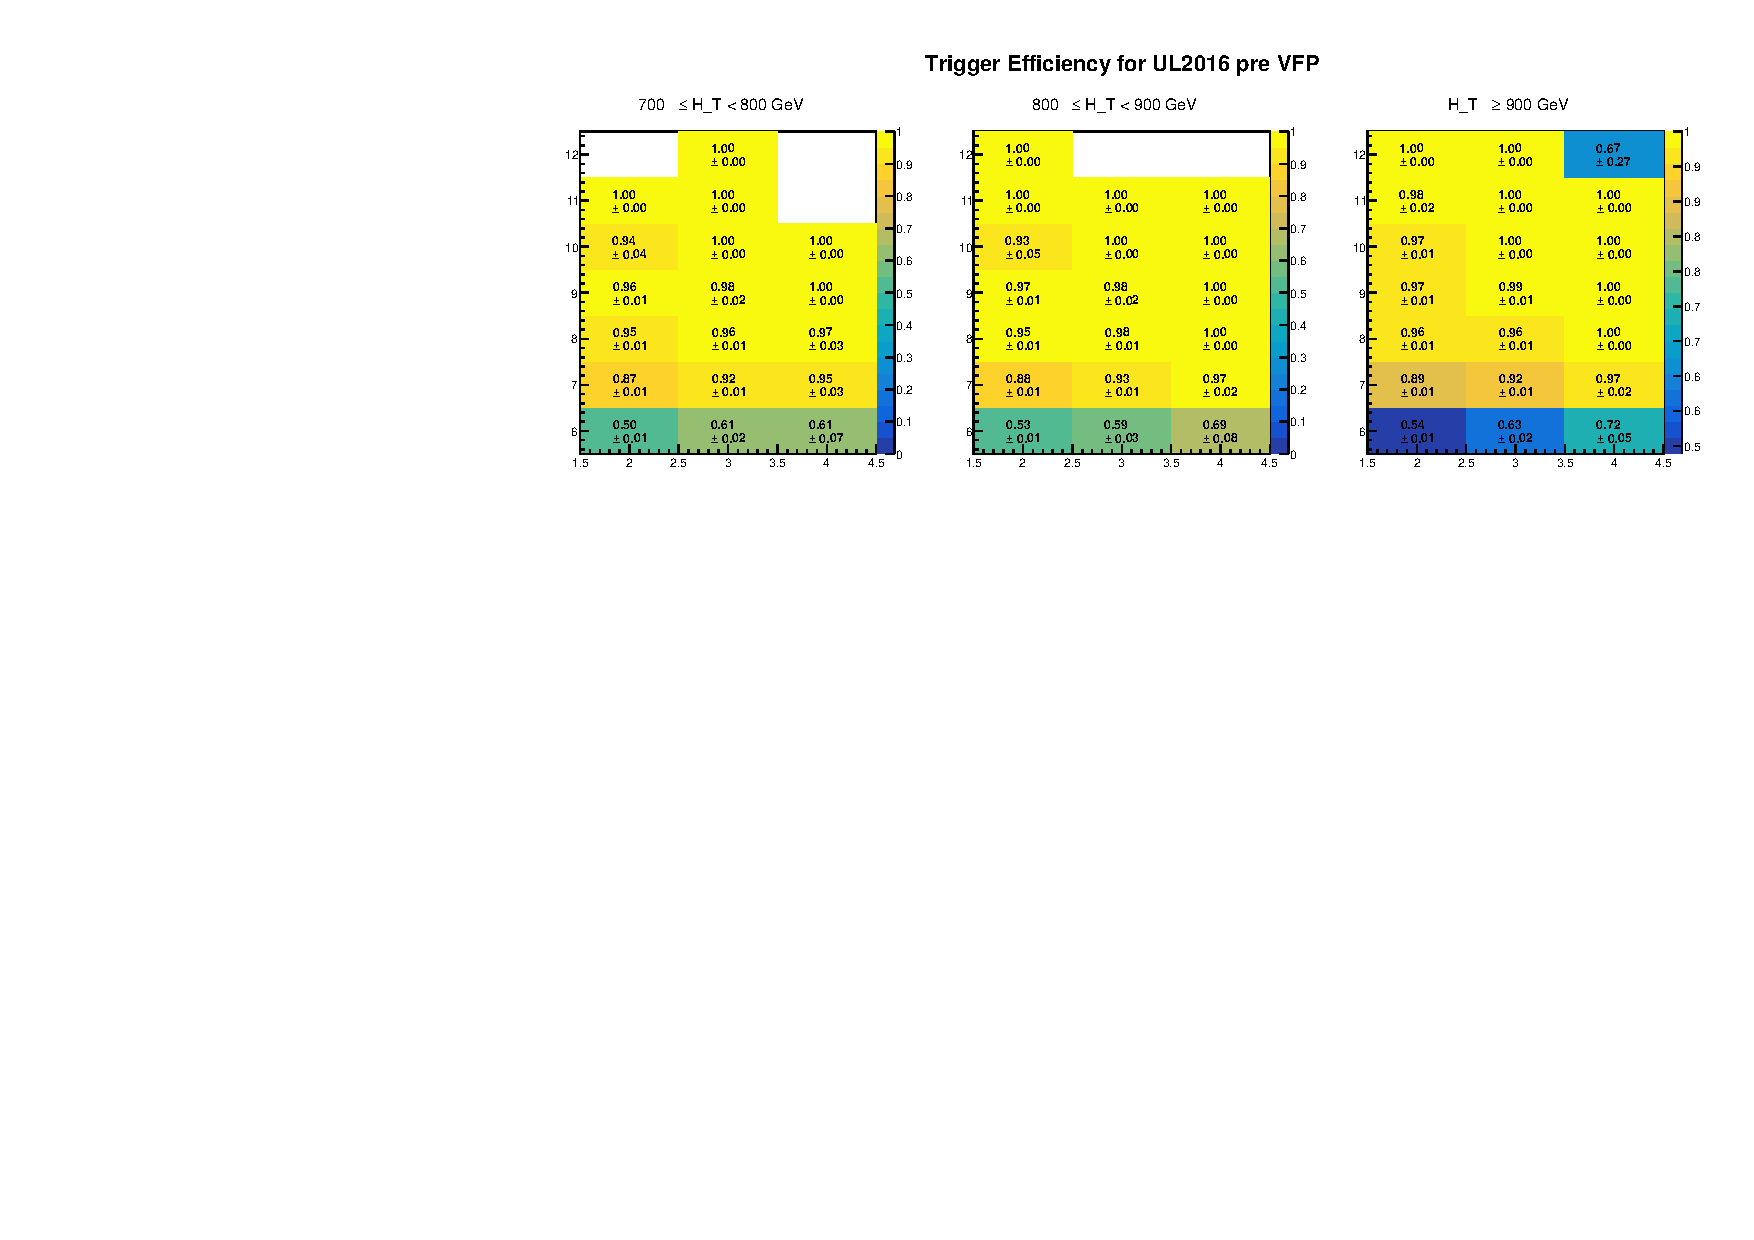
\includegraphics[width=.4\columnwidth]{plots/Trigger/2016_preVFP.pdf}
    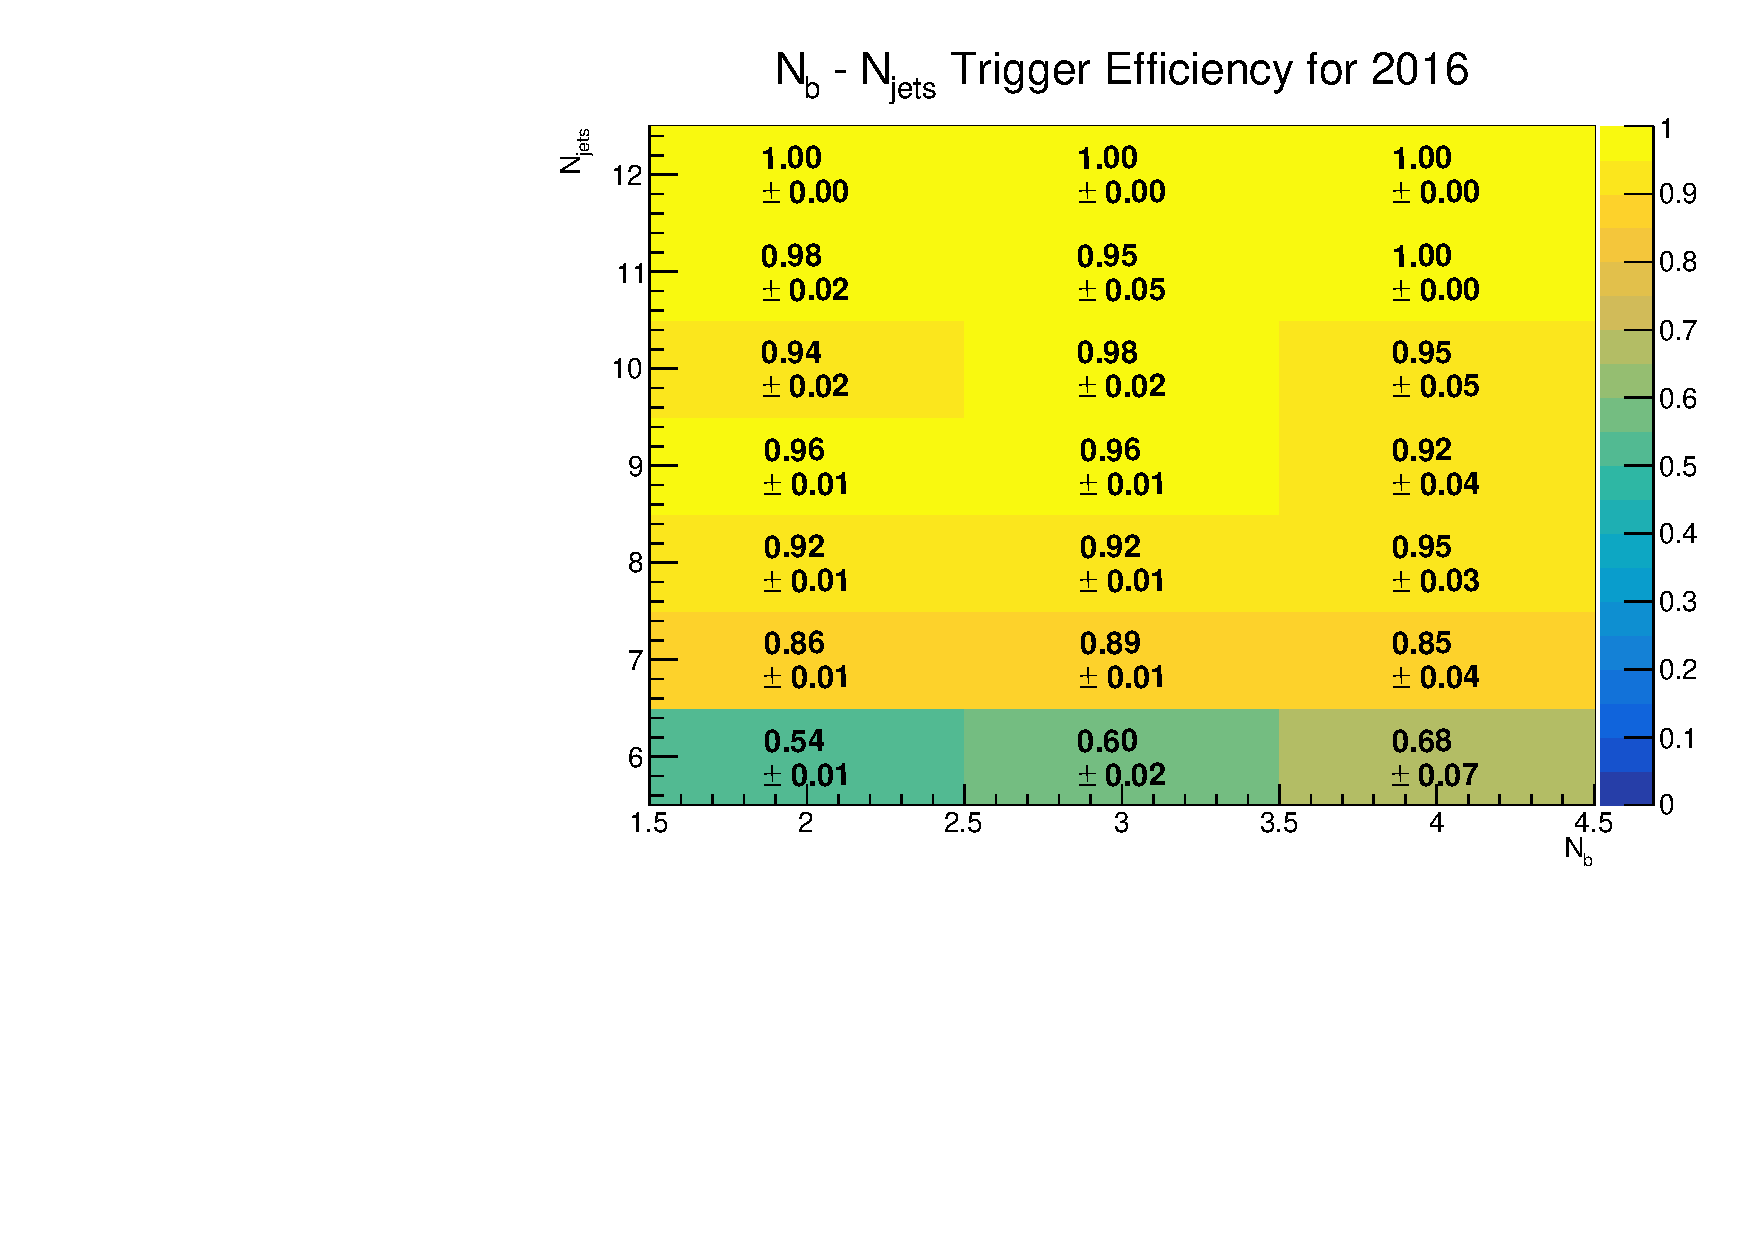
\includegraphics[width=.4\columnwidth]{plots/Trigger/2016.pdf}
    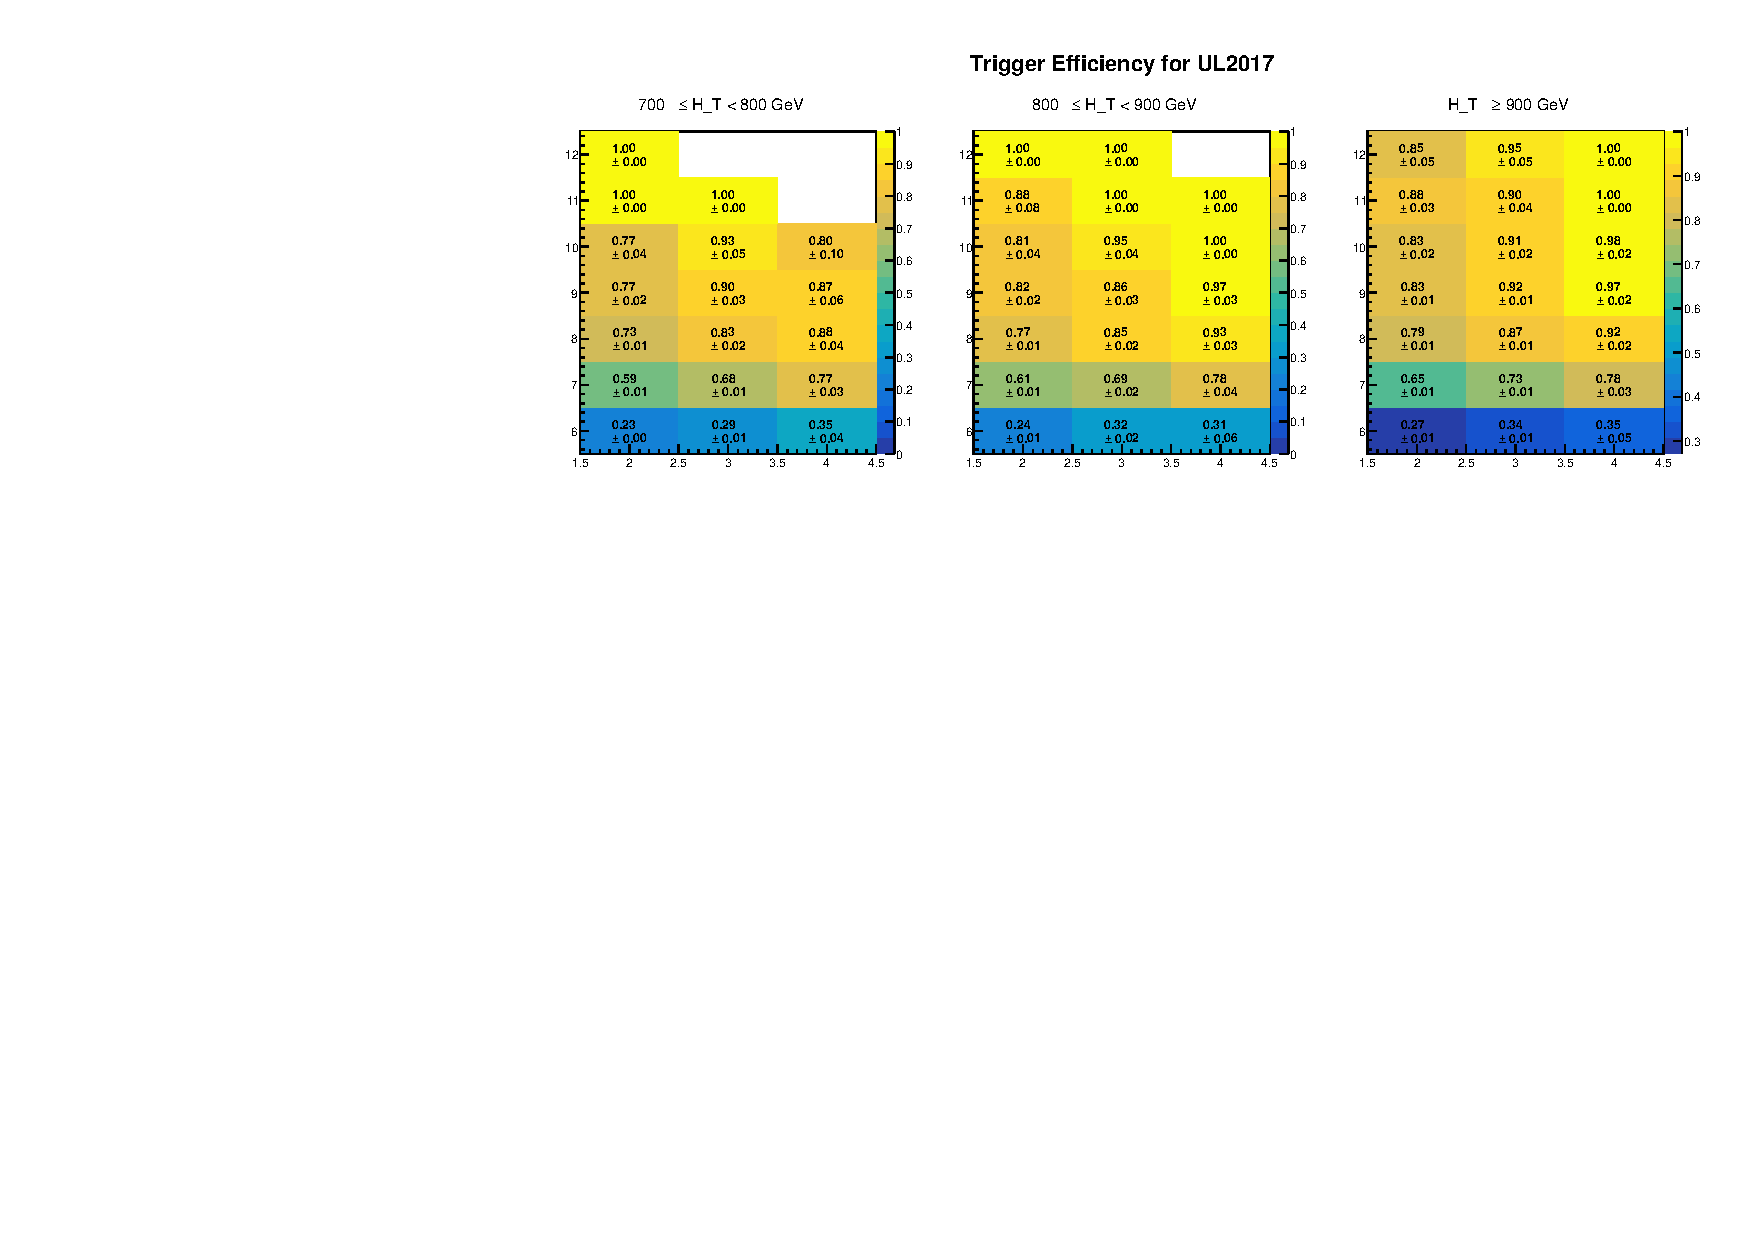
\includegraphics[width=.4\columnwidth]{plots/Trigger/2017.pdf}
    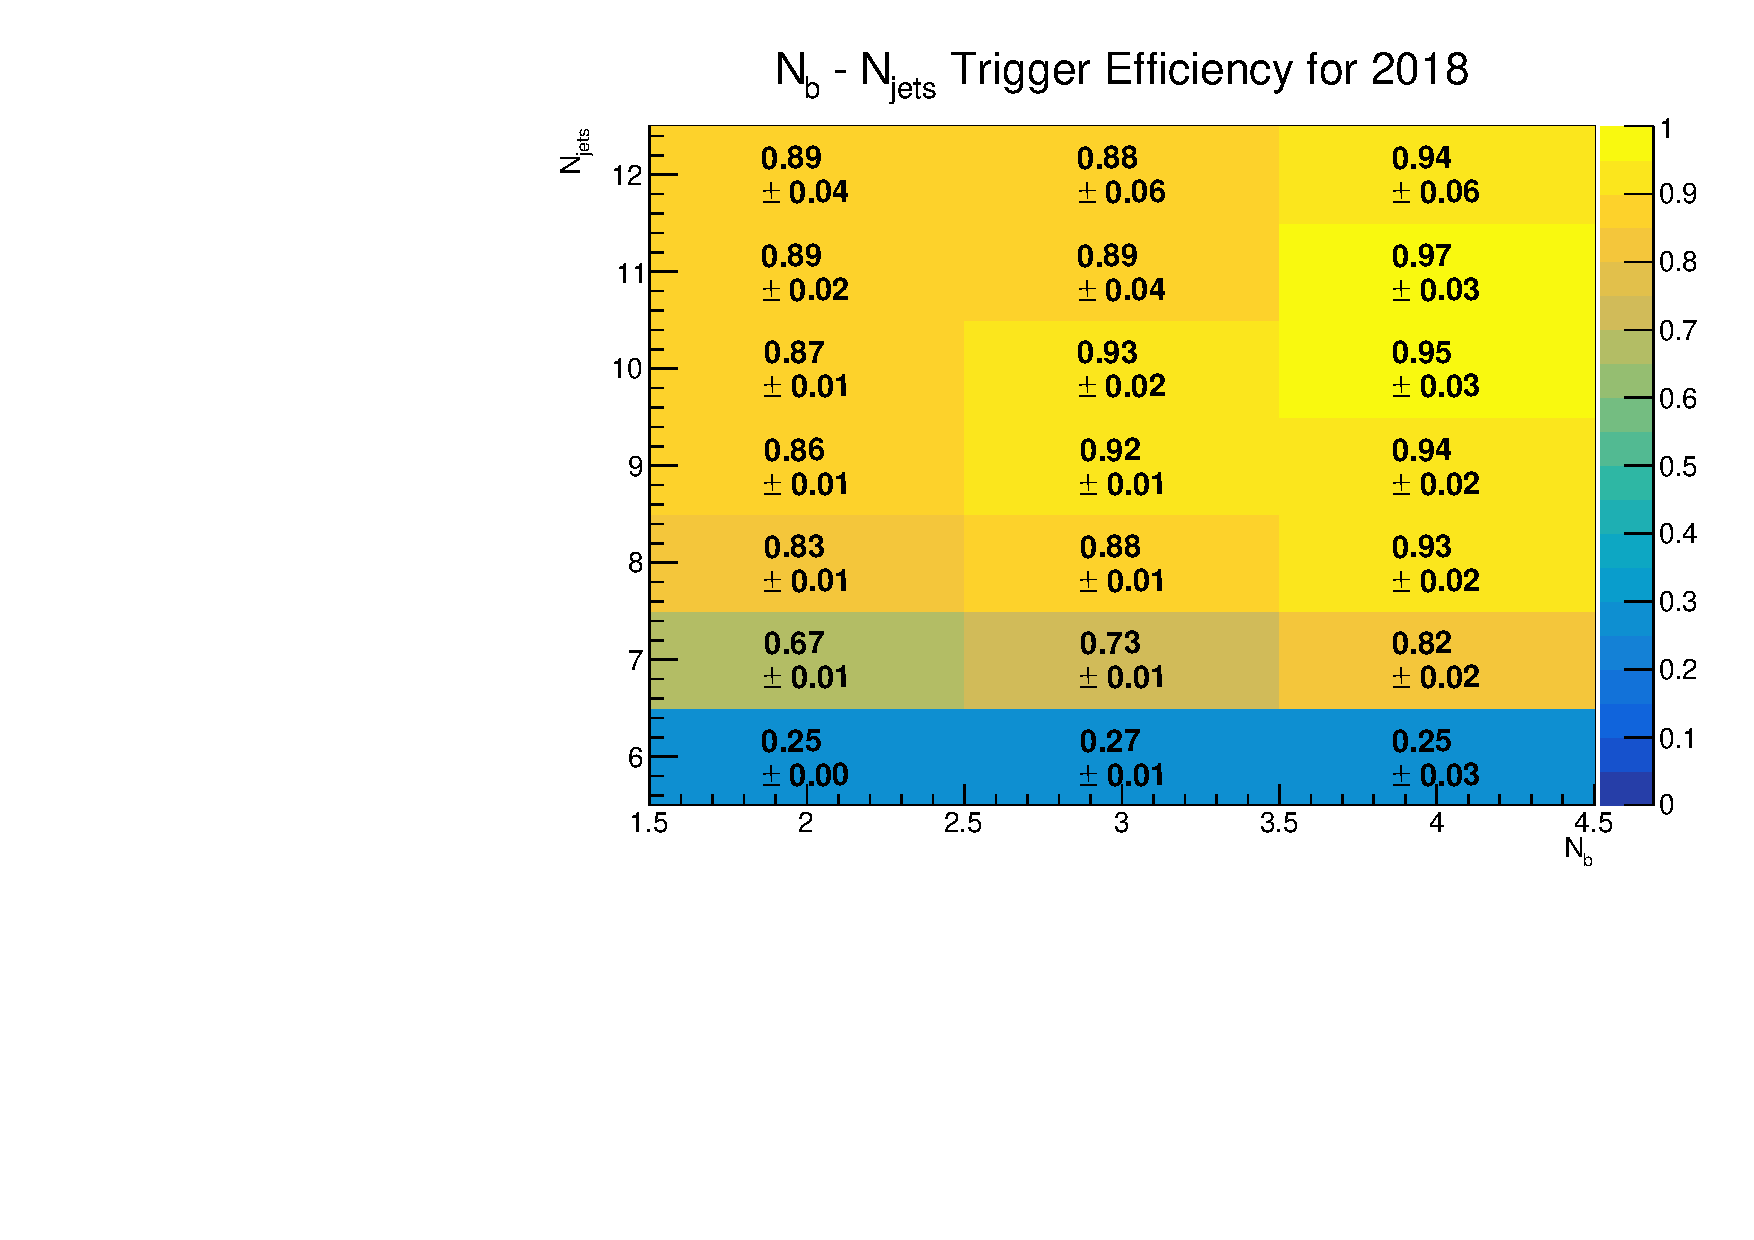
\includegraphics[width=.4\columnwidth]{plots/Trigger/2018.pdf}
    
    \caption{Efficiency measured for search triggers as a function of $N_{jet}$ and $N_{b-jet}$ for 2016 pre VFP, 2016 post VFP, 2017 and 2018 data. The $N_{jet}$ = 6 region used for the validation test is shown as well.}
    \label{figure_1} 
\end{figure}

\begin{figure}[!t]
    \centering
    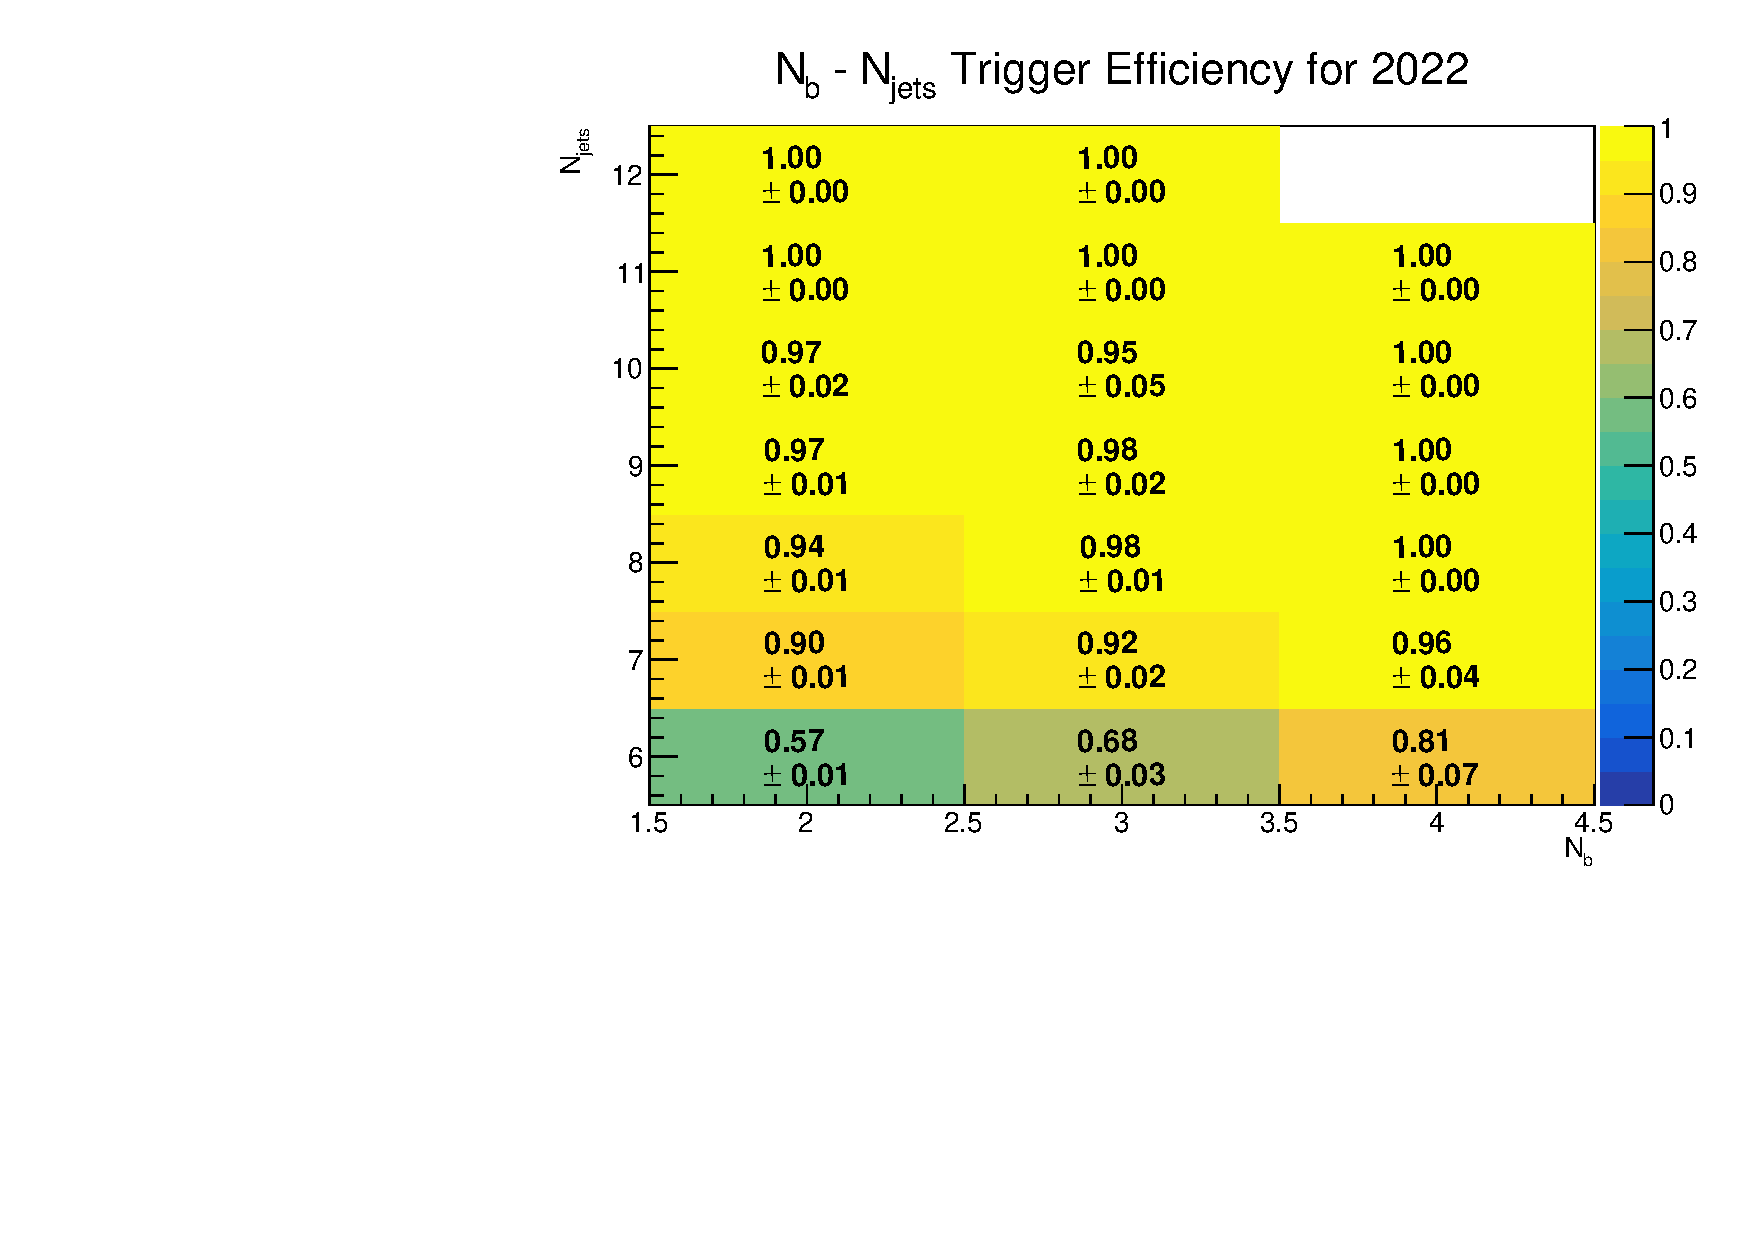
\includegraphics[width=.4\columnwidth]{plots/Trigger/2022.pdf}
    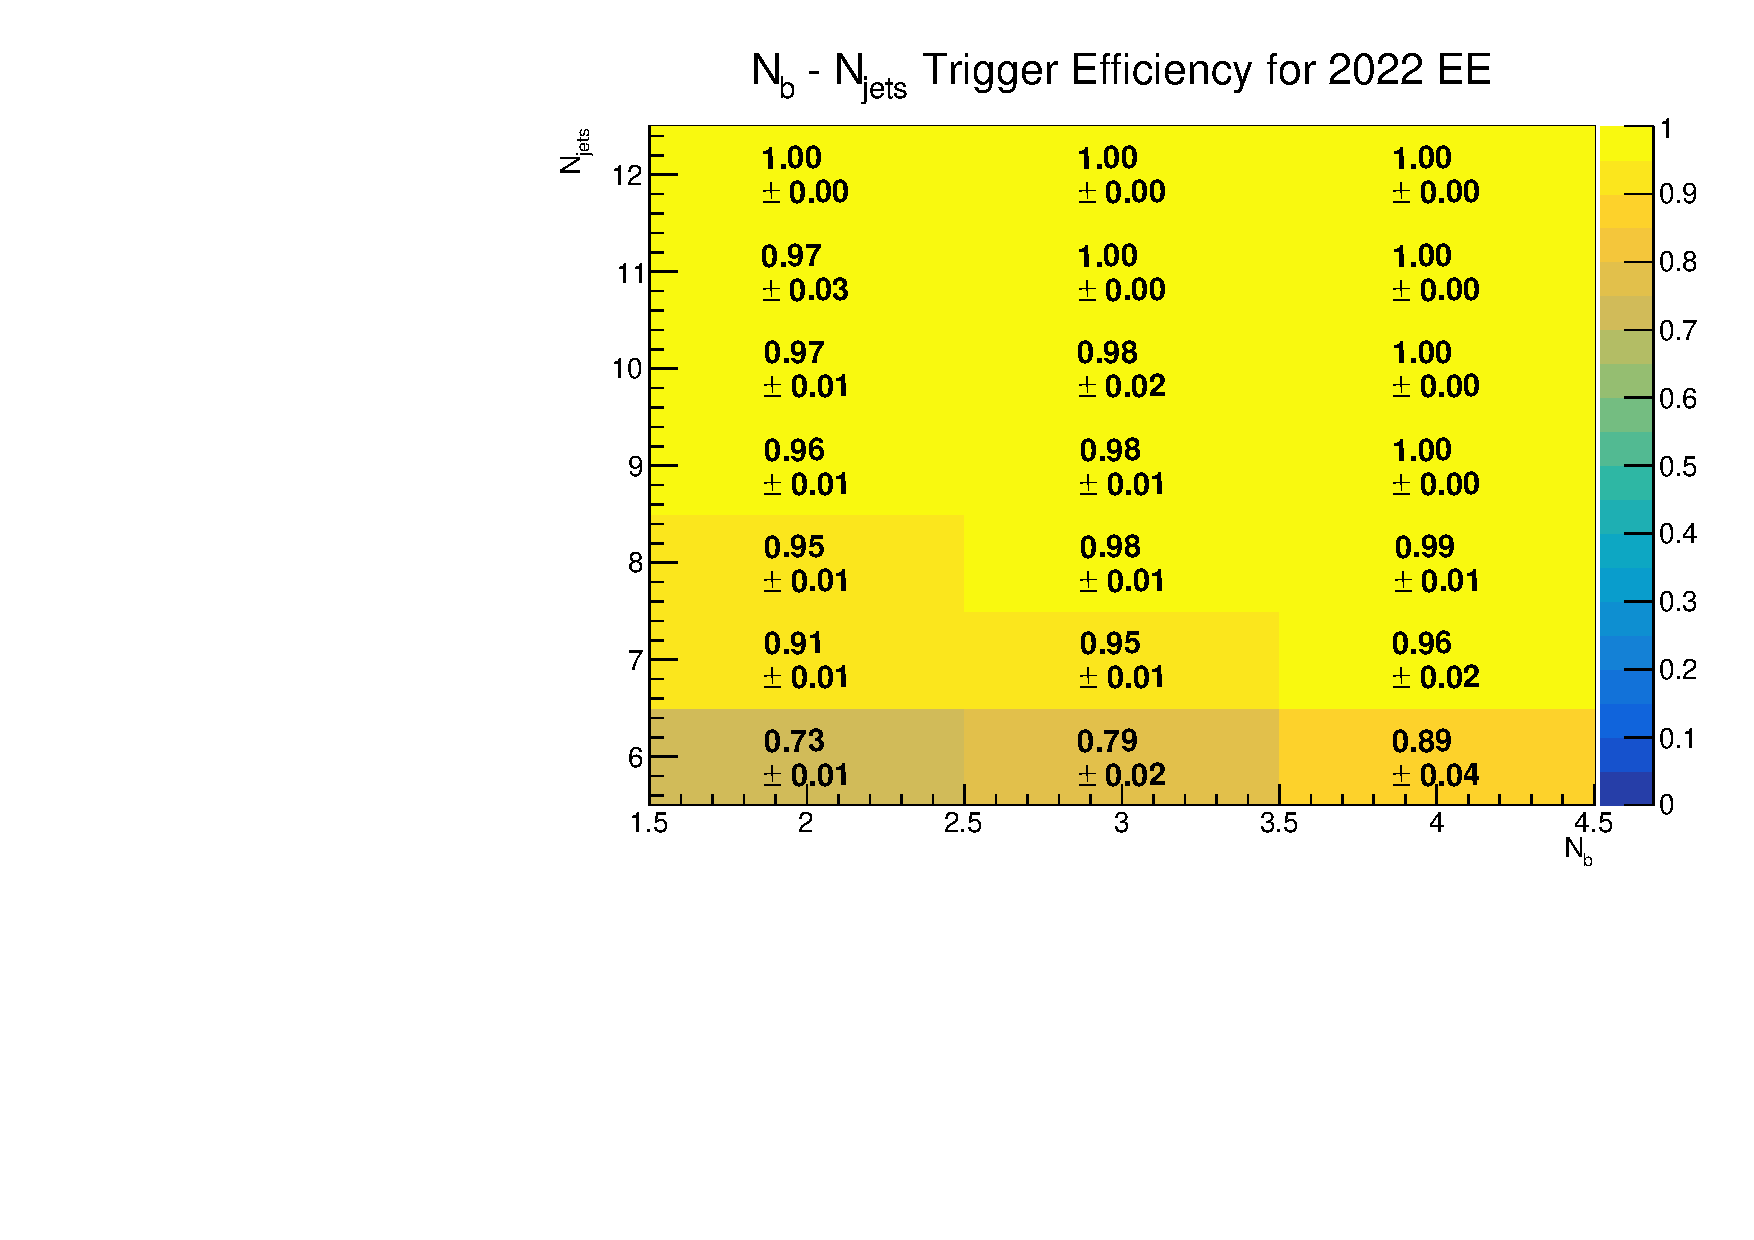
\includegraphics[width=.4\columnwidth]{plots/Trigger/2022EE.pdf}
    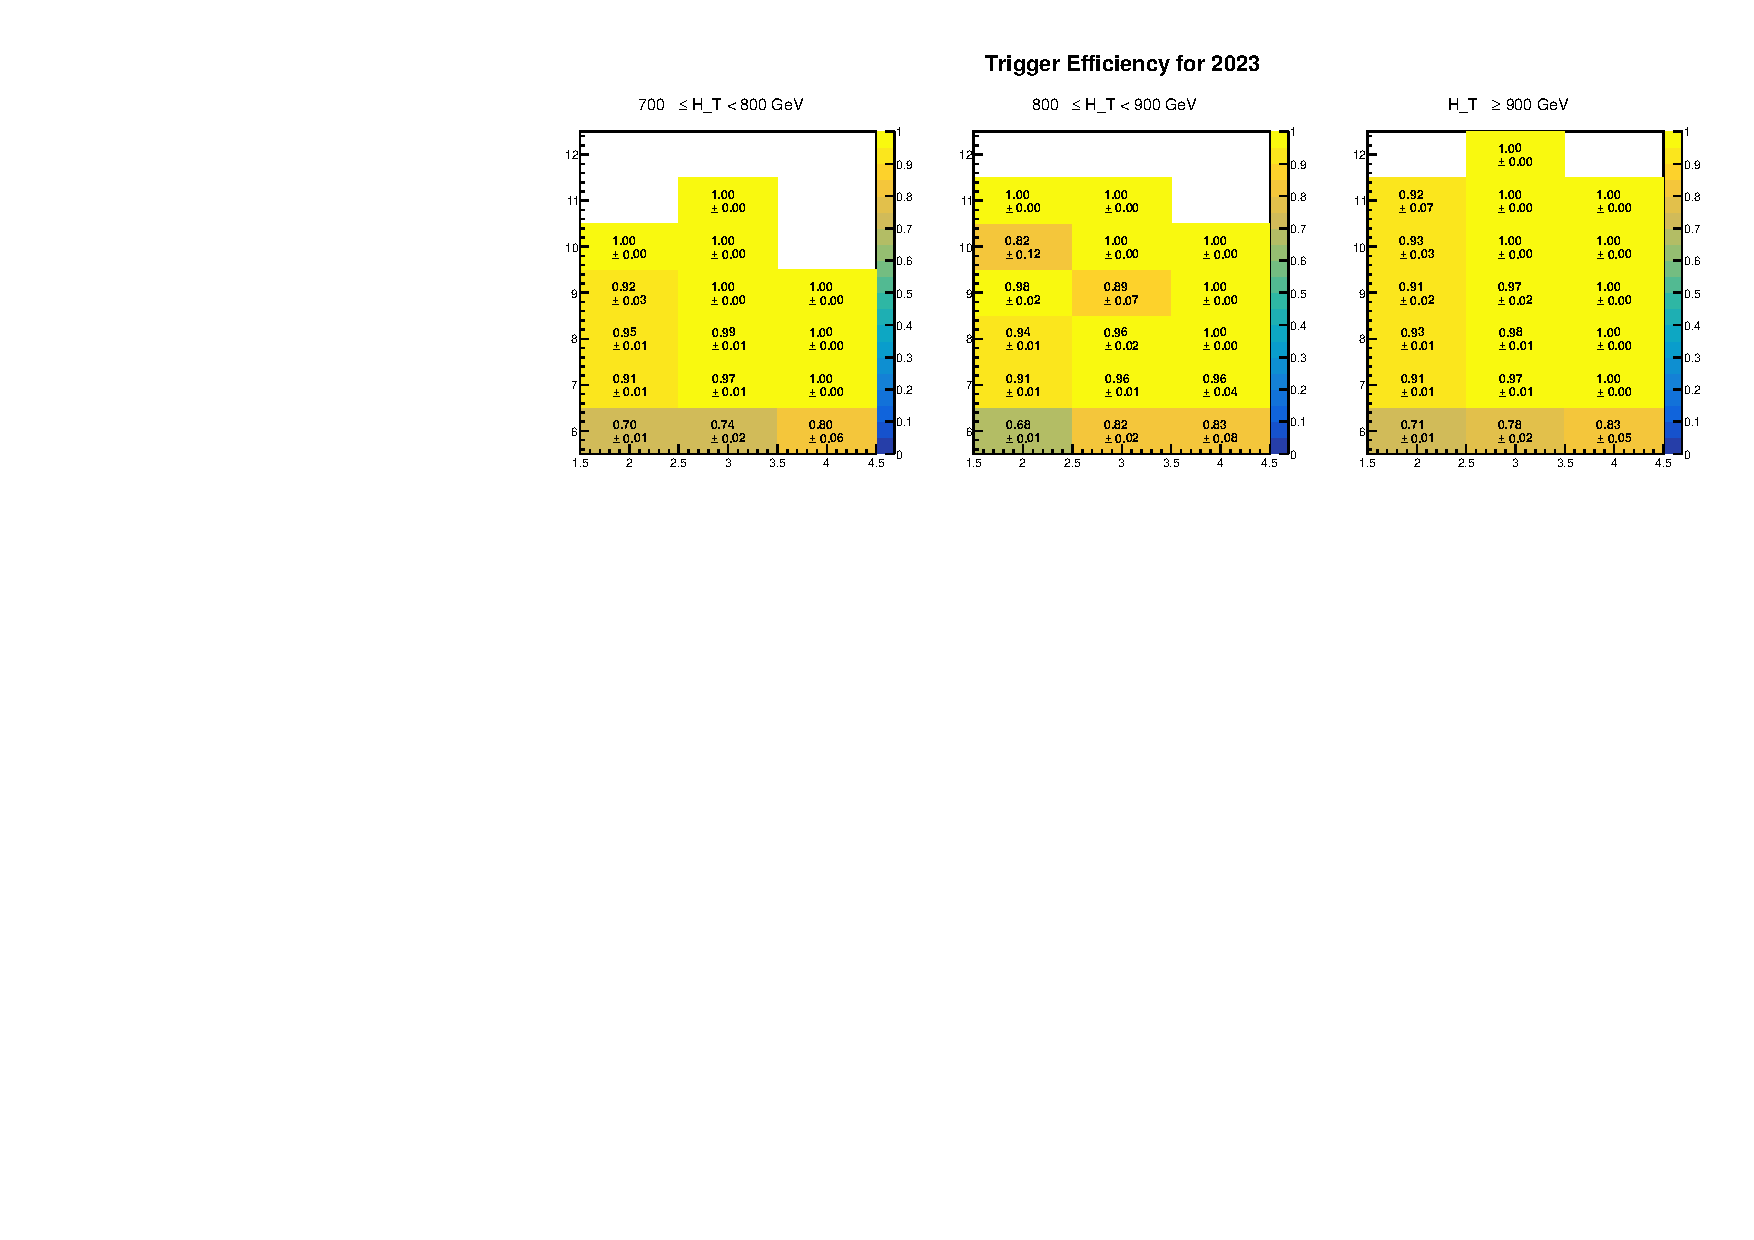
\includegraphics[width=.4\columnwidth]{plots/Trigger/2023.pdf}
    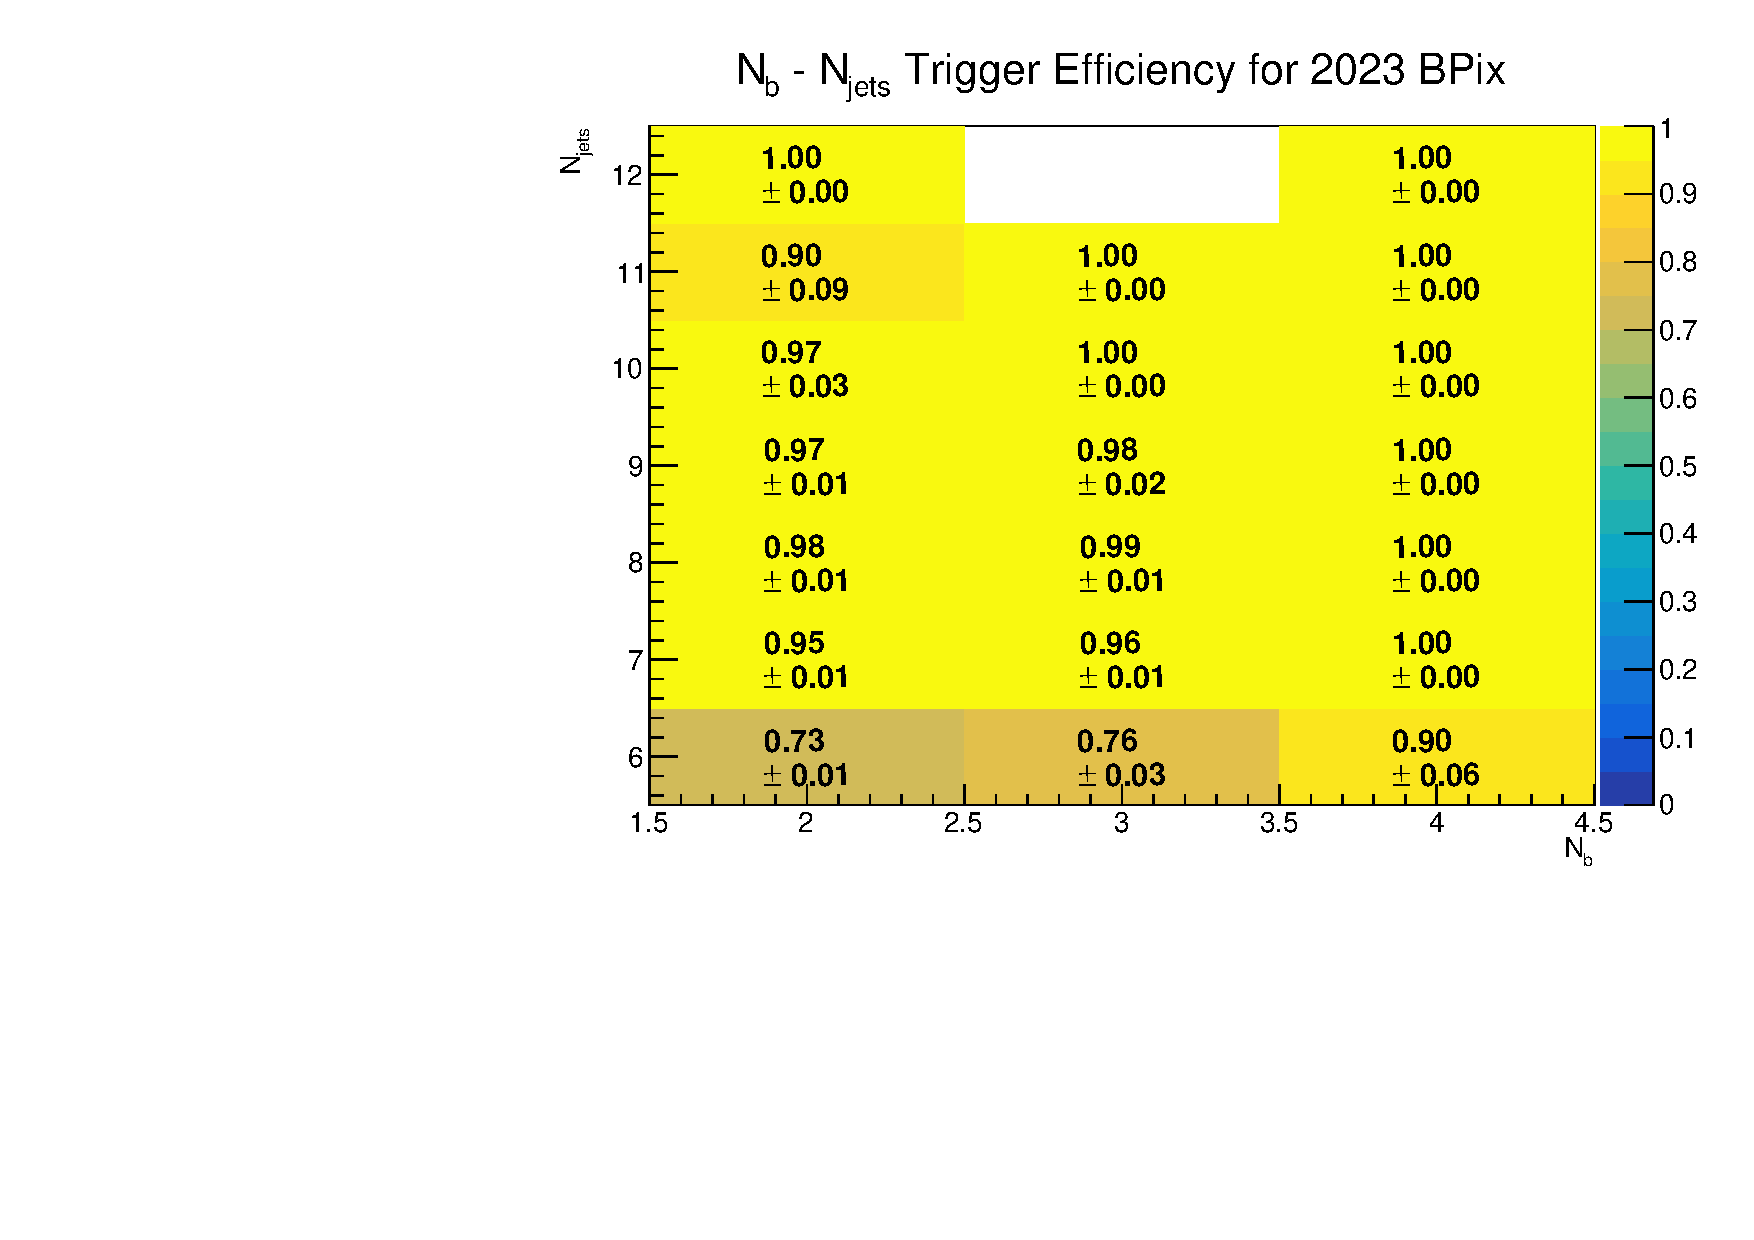
\includegraphics[width=.4\columnwidth]{plots/Trigger/2023BPix.pdf}
    
    \caption{Efficiency measured for search triggers as a function of $N_{jet}$ and $N_{b-jet}$ for 2016 pre VFP, 2016 post VFP, 2017 and 2018 data. The $N_{jet}$ = 6 region used for the validation test is shown as well.}
    \label{figure_1} 
\end{figure}
The datasets used for measuring trigger efficiency, as listed in Tables 3 and 4, include events that have passed the isolated muon trigger.
\begin{table}[]
\caption{ Dataset used for run2 trigger efficiency measurement}
\centering
\begin{tabular}{|c|l|}
\hline
Year                               & \multicolumn{1}{c|}{Dataset}                                                                                                                                                                                                                                                                                                                                                                         \\ \hline
\multicolumn{1}{|l|}{2016 pre VFP} & \begin{tabular}[c]{@{}l@{}}/SingleMuon/Run2016B-ver1\_HIPM\_UL2016\_MiniAODv2\_NanoAODv9-v2/NANOAOD\\ /SingleMuon/Run2016C-HIPM\_UL2016\_MiniAODv2\_NanoAODv9-v2/NANOAOD\\ /SingleMuon/Run2016D-HIPM\_UL2016\_MiniAODv2\_NanoAODv9-v2/NANOAOD\\ /SingleMuon/Run2016E-HIPM\_UL2016\_MiniAODv2\_NanoAODv9-v2/NANOAOD\\ /SingleMuon/Run2016F-HIPM\_UL2016\_MiniAODv2\_NanoAODv9-v2/NANOAOD\end{tabular} \\ \hline
2016 post VFP                      & \begin{tabular}[c]{@{}l@{}}/SingleMuon/Run2016F-UL2016\_MiniAODv2\_NanoAODv9-v1/NANOAOD\\ /SingleMuon/Run2016G-UL2016\_MiniAODv2\_NanoAODv9-v1/NANOAOD\\ /SingleMuon/Run2016H-UL2016\_MiniAODv2\_NanoAODv9-v1/NANOAOD\end{tabular}                                                                                                                                                                   \\ \hline
2017                               & \begin{tabular}[c]{@{}l@{}}/SingleMuon/Run2017B-UL2017\_MiniAODv2\_NanoAODv9-v1/NANOAOD\\ /SingleMuon/Run2017C-UL2017\_MiniAODv2\_NanoAODv9-v1/NANOAOD\\ /SingleMuon/Run2017D-UL2017\_MiniAODv2\_NanoAODv9-v1/NANOAOD\\ /SingleMuon/Run2017E-UL2017\_MiniAODv2\_NanoAODv9-v1/NANOAOD\\ /SingleMuon/Run2017F-UL2017\_MiniAODv2\_NanoAODv9-v1/NANOAOD\end{tabular}                                     \\ \hline
2018                               & \begin{tabular}[c]{@{}l@{}}/SingleMuon/Run2018A-UL2018\_MiniAODv2\_NanoAODv9-v2/NANOAOD\\ /SingleMuon/Run2018B-UL2018\_MiniAODv2\_NanoAODv9-v2/NANOAOD\\ /SingleMuon/Run2018C-UL2018\_MiniAODv2\_NanoAODv9-v2/NANOAOD\\ /SingleMuon/Run2018D-UL2018\_MiniAODv2\_NanoAODv9-v1/NANOAOD\end{tabular}                                                                                                    \\ \hline
\end{tabular}
\end{table}
\begin{table}[]
\caption{ Dataset used for early run3 trigger efficiency measurement}
\centering
\begin{tabular}{|c|l|}
\hline
Year                         & \multicolumn{1}{c|}{Trigger path}                                                                                                                                                                                                                                                                                                                                                             \\ \hline
2022                         & \begin{tabular}[c]{@{}l@{}}/Muon/Run2022C-22Sep2023-v1/NANOAOD\\ /Muon/Run2022D-22Sep2023-v1/NANOAOD\end{tabular}                                                                                                                                                                                                                                                                             \\ \hline
\multicolumn{1}{|l|}{2022EE} & \begin{tabular}[c]{@{}l@{}}/Muon/Run2022E-22Sep2023-v1/NANOAOD\\ /Muon/Run2022F-22Sep2023-v2/NANOAOD\\ /Muon/Run2022G-22Sep2023-v1/NANOAOD\end{tabular}                                                                                                                                                                                                                                       \\ \hline
2023                         & \begin{tabular}[c]{@{}l@{}}/Muon0/Run2023C-22Sep2023\_v1-v1/NANOAOD\\ /Muon0/Run2023C-22Sep2023\_v2-v1/NANOAOD\\ /Muon0/Run2023C-22Sep2023\_v3-v1/NANOAOD\\ /Muon0/Run2023C-22Sep2023\_v4-v1/NANOAOD\\ /Muon1/Run2023C-22Sep2023\_v1-v1/NANOAOD\\ /Muon1/Run2023C-22Sep2023\_v2-v1/NANOAOD\\ /Muon1/Run2023C-22Sep2023\_v3-v1/NANOAOD\\ /Muon1/Run2023C-22Sep2023\_v4-v1/NANOAOD\end{tabular} \\ \hline
2023BPix                     & \begin{tabular}[c]{@{}l@{}}/Muon0/Run2023D-22Sep2023\_v1-v1/NANOAOD\\ /Muon0/Run2023D-22Sep2023\_v2-v1/NANOAOD\\ /Muon1/Run2023D-22Sep2023\_v1-v1/NANOAOD\\ /Muon1/Run2023D-22Sep2023\_v2-v1/NANOAOD\end{tabular}                                                                                                                                                                             \\ \hline
\end{tabular}
\end{table}
Figure 1 and 2 show the measured efficiency in the $N_{jet} $ and $ N_{b-jet}$ plane for each year. There is a clear dependence on $N_{jet} $ and $ N_{b-jet}$, which justifies the necessity of corrections depending on $N_{jet} $ and $ N_{b-jet}$. The bottom row corresponds to $N_{jet} = 6$ and shows low efficiencies due to the requirement of $N_{jet} \geq 6$ in trigger paths. This region is used only for the validation of the background estimation methods. Details will be discussed in Section 5. 
\begin{figure}[!t]
    \centering
    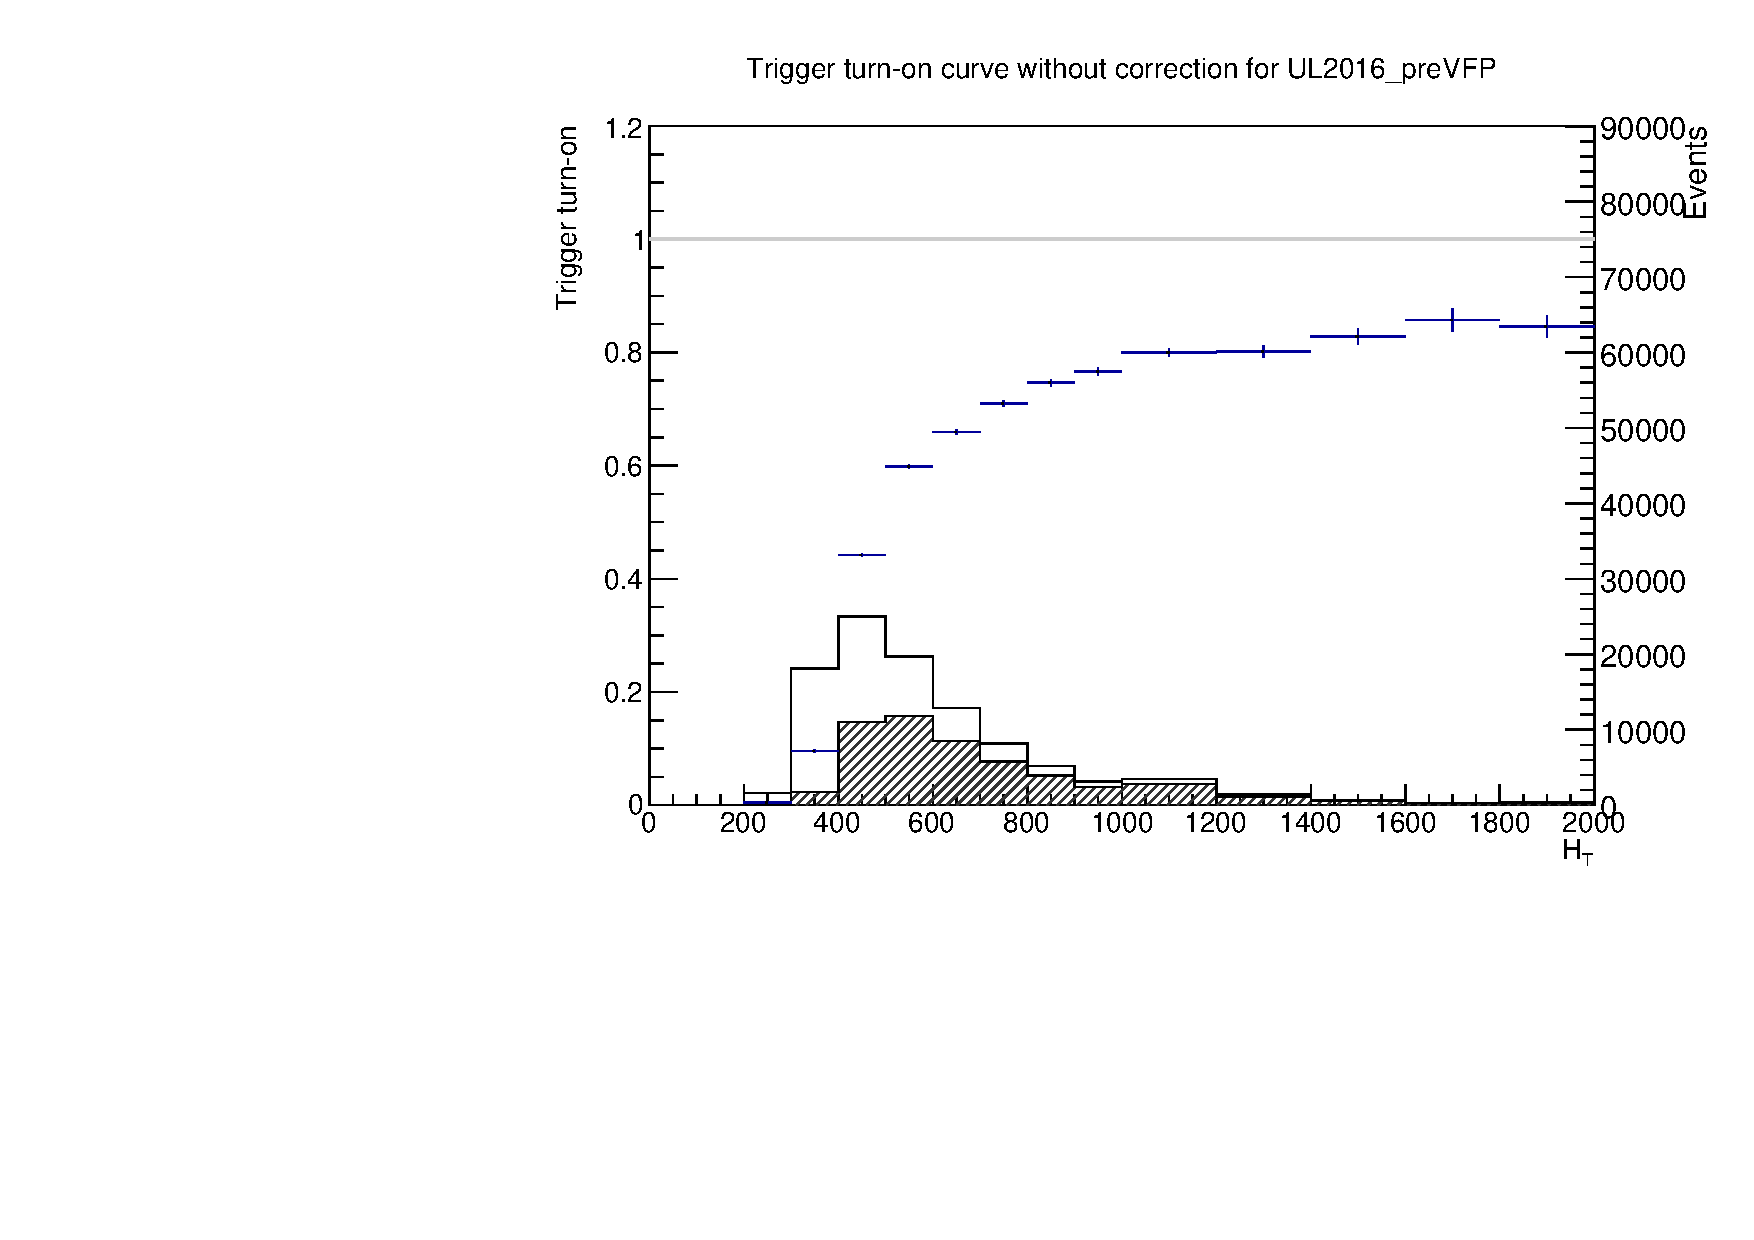
\includegraphics[width=.24\columnwidth]{plots/Trigger/turnOn_UL2016_preVFP_Coroff.pdf}
    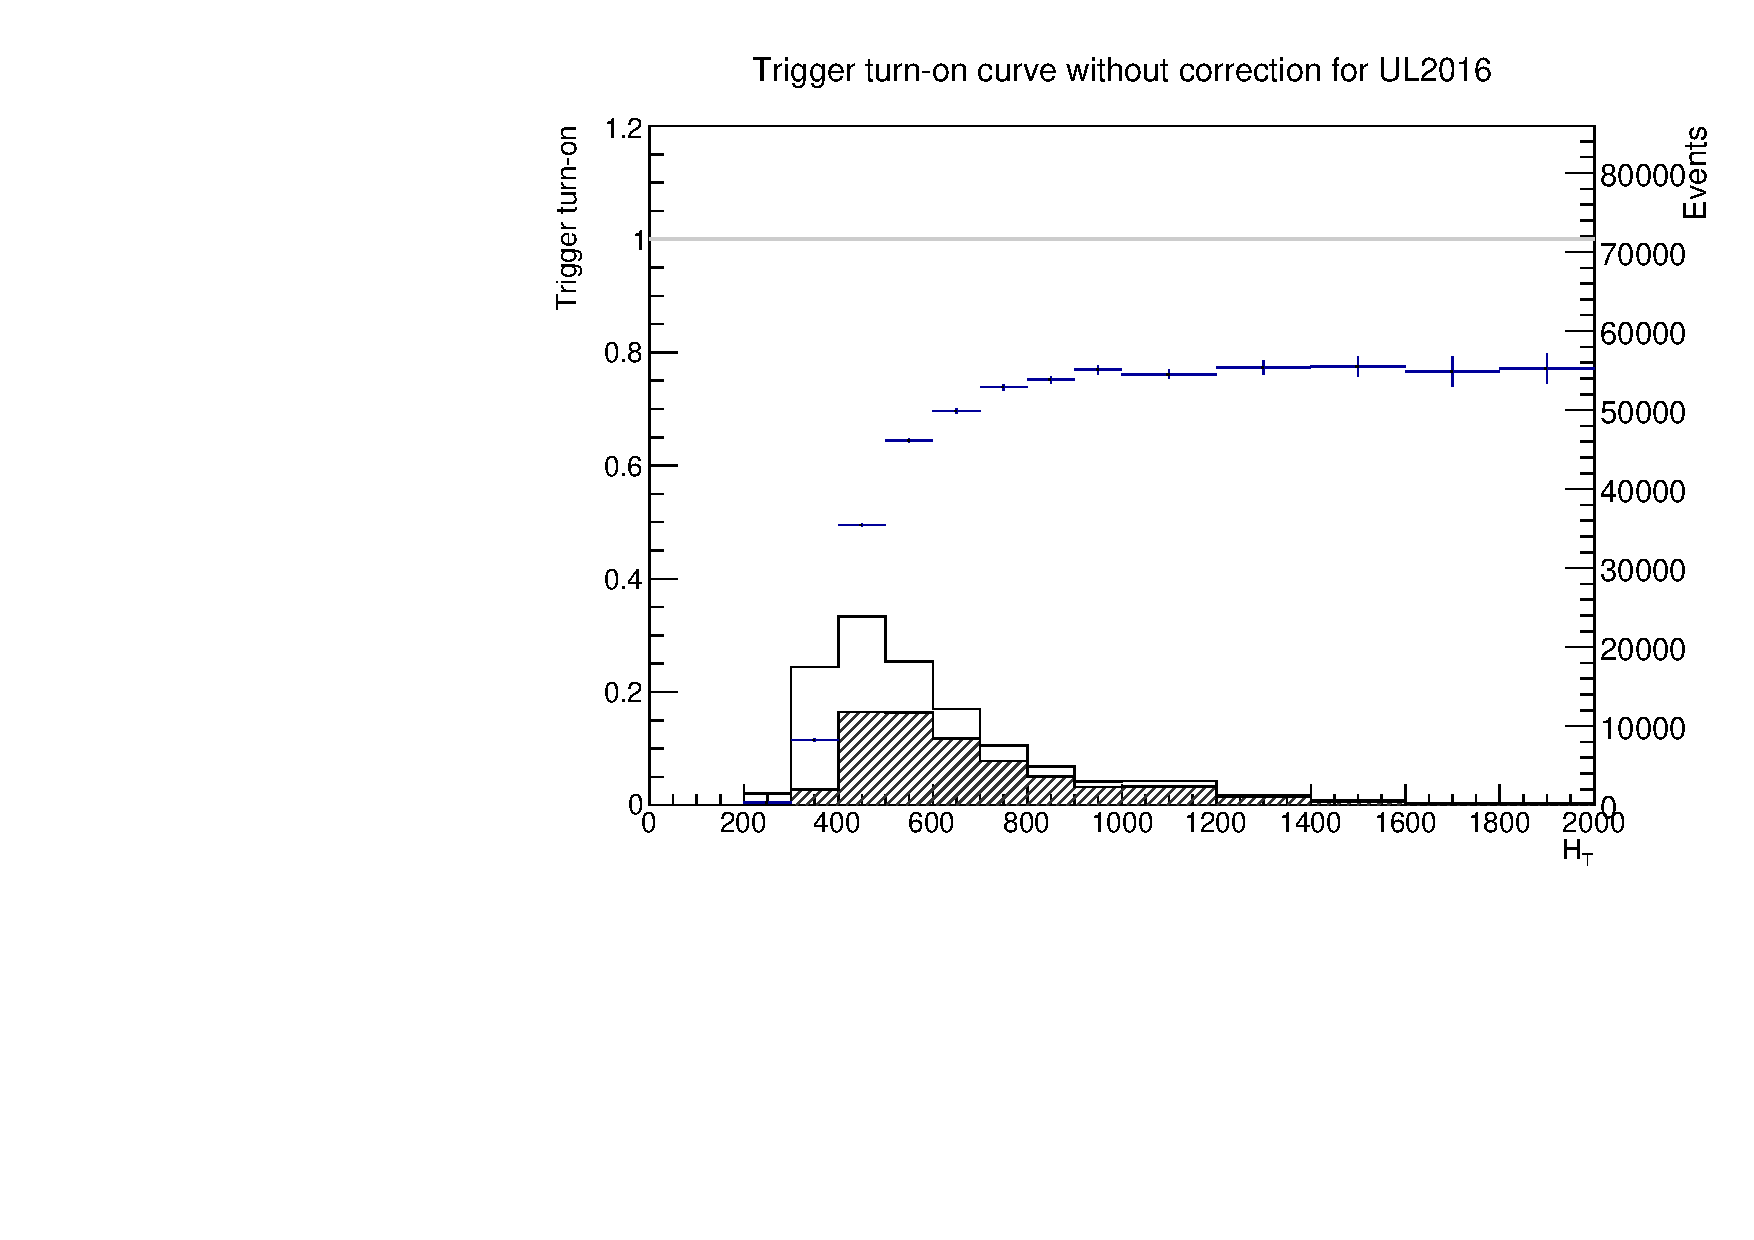
\includegraphics[width=.24\columnwidth]{plots/Trigger/turnOn_UL2016_Coroff.pdf}
    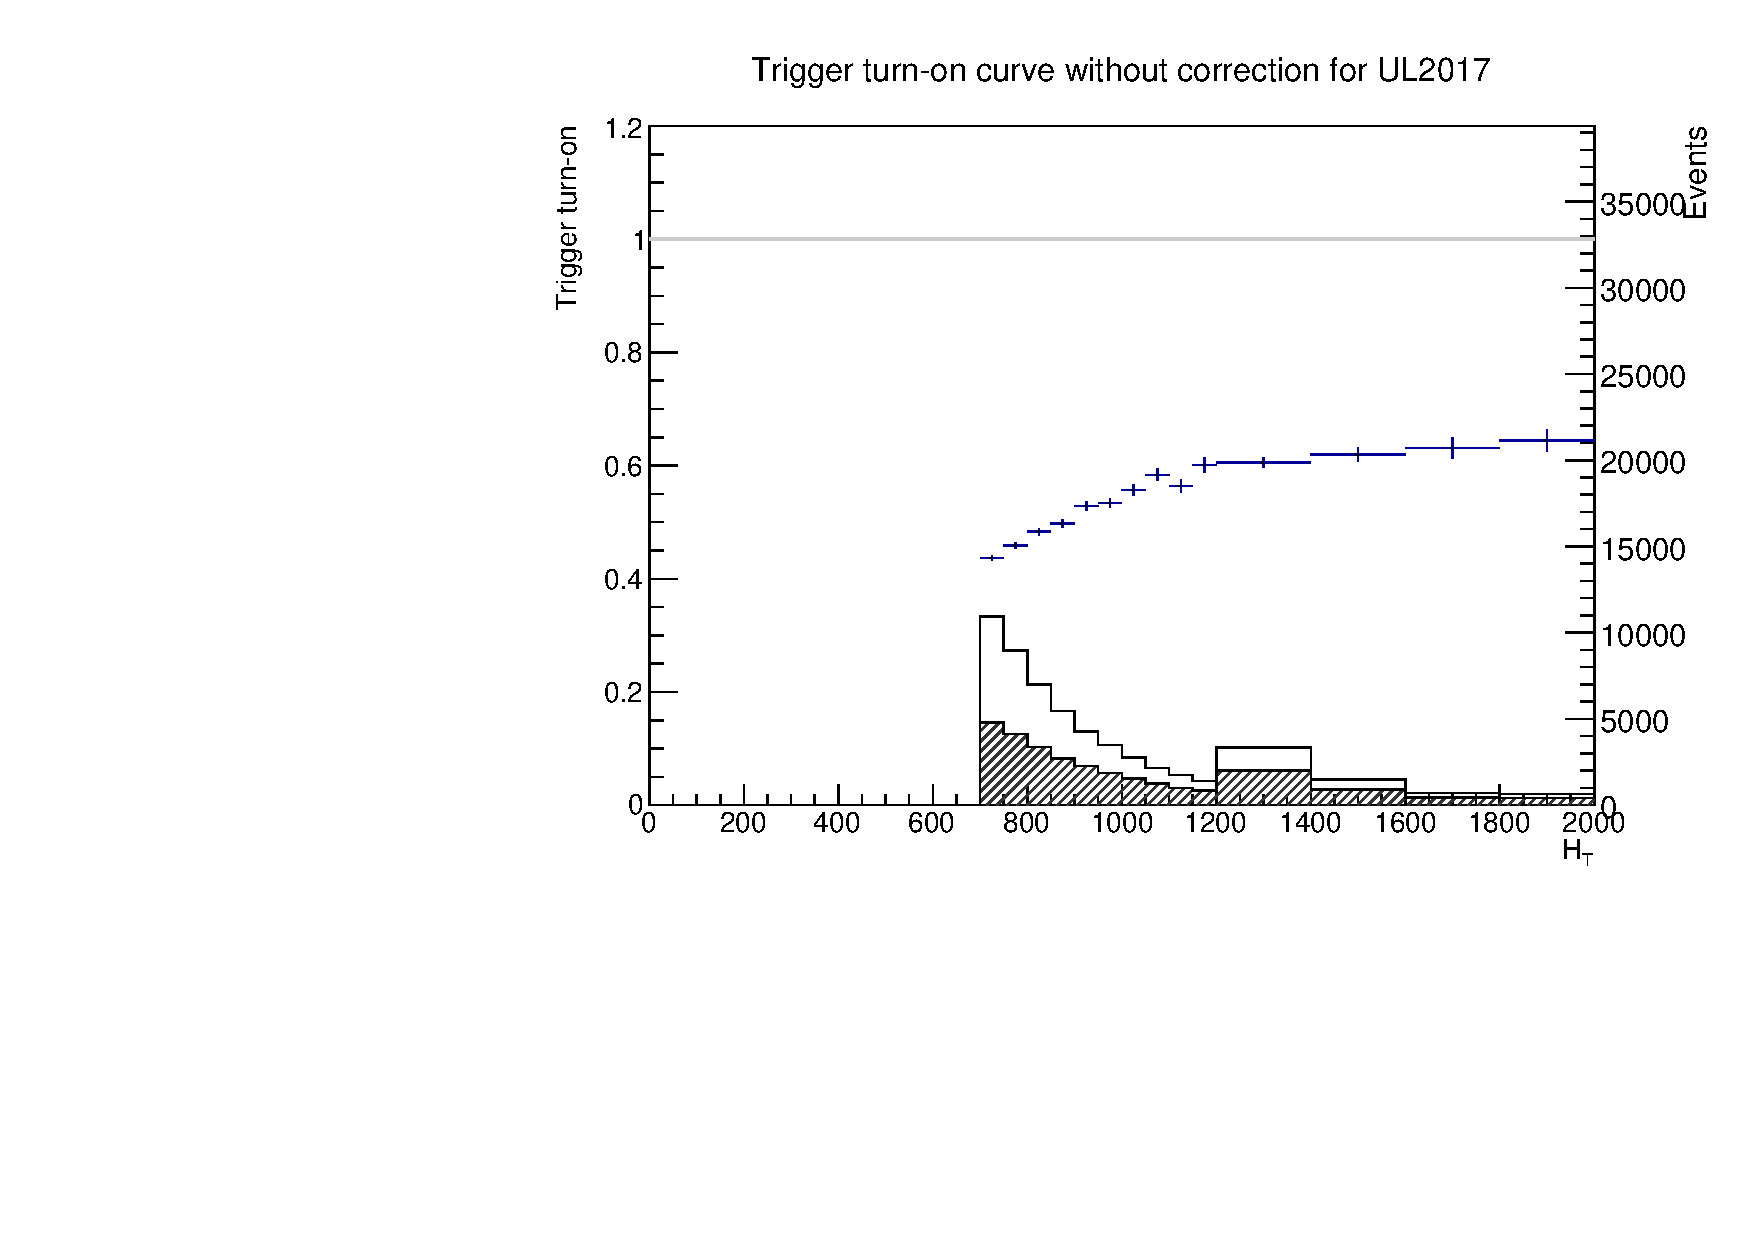
\includegraphics[width=.24\columnwidth]{plots/Trigger/turnOn_UL2017_Coroff.pdf}
    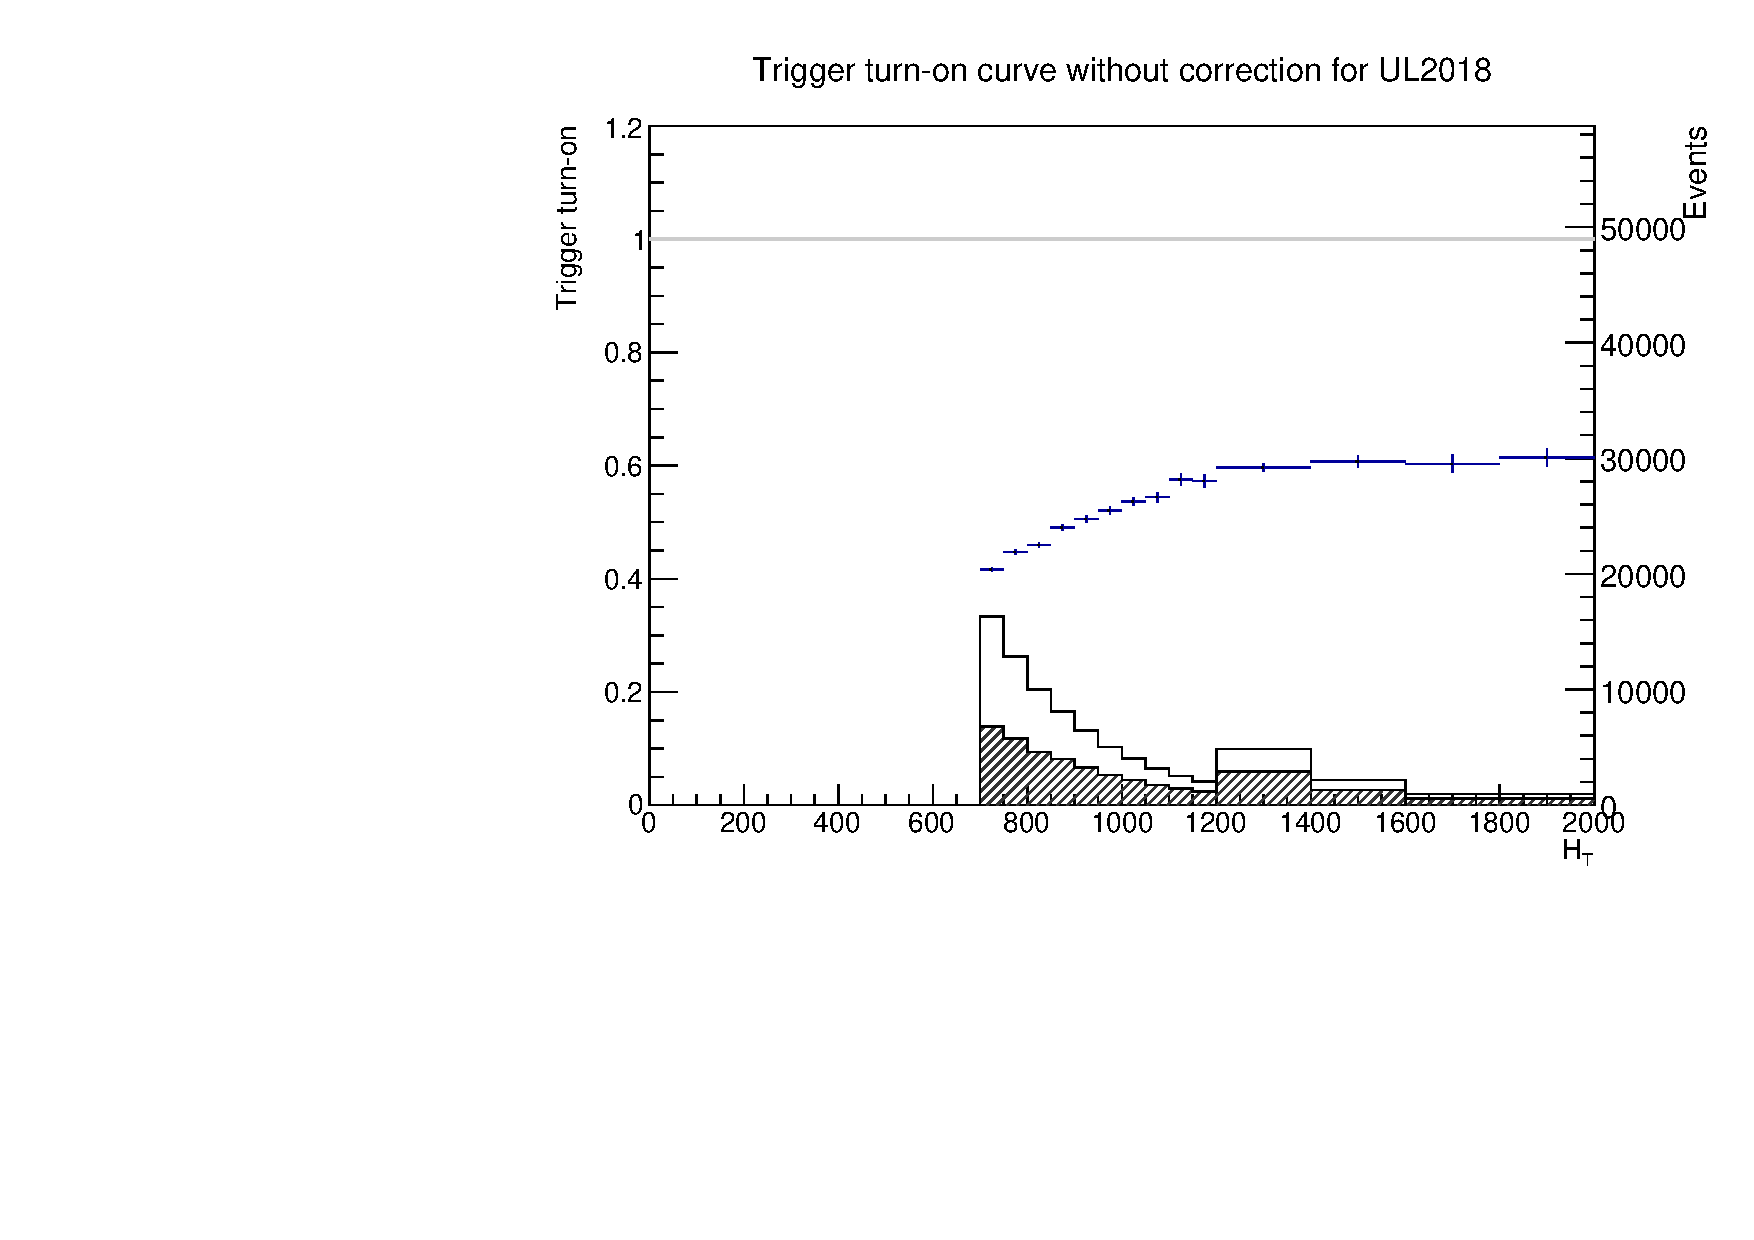
\includegraphics[width=.24\columnwidth]{plots/Trigger/turnOn_UL2018_Coroff.pdf}
    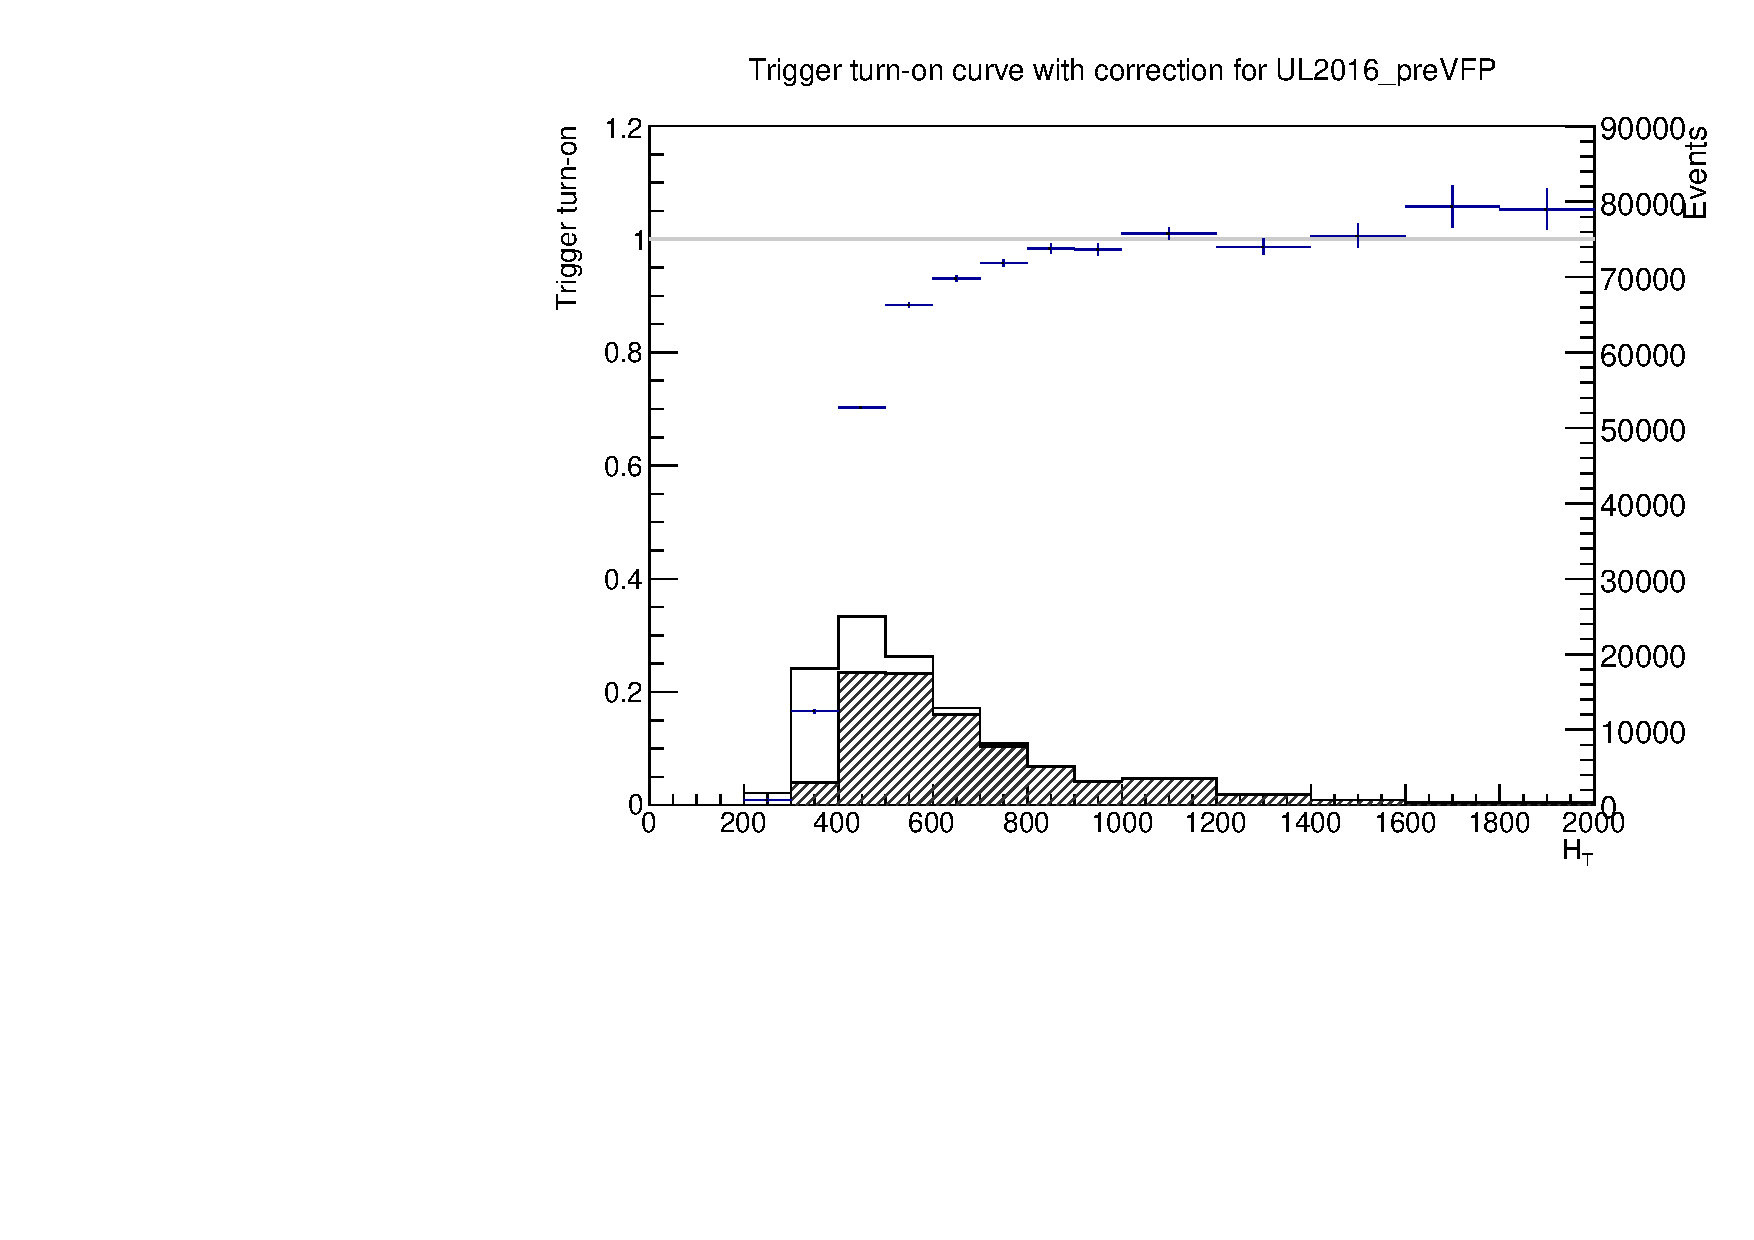
\includegraphics[width=.24\columnwidth]{plots/Trigger/turnOn_UL2016_preVFP_Coron.pdf}
    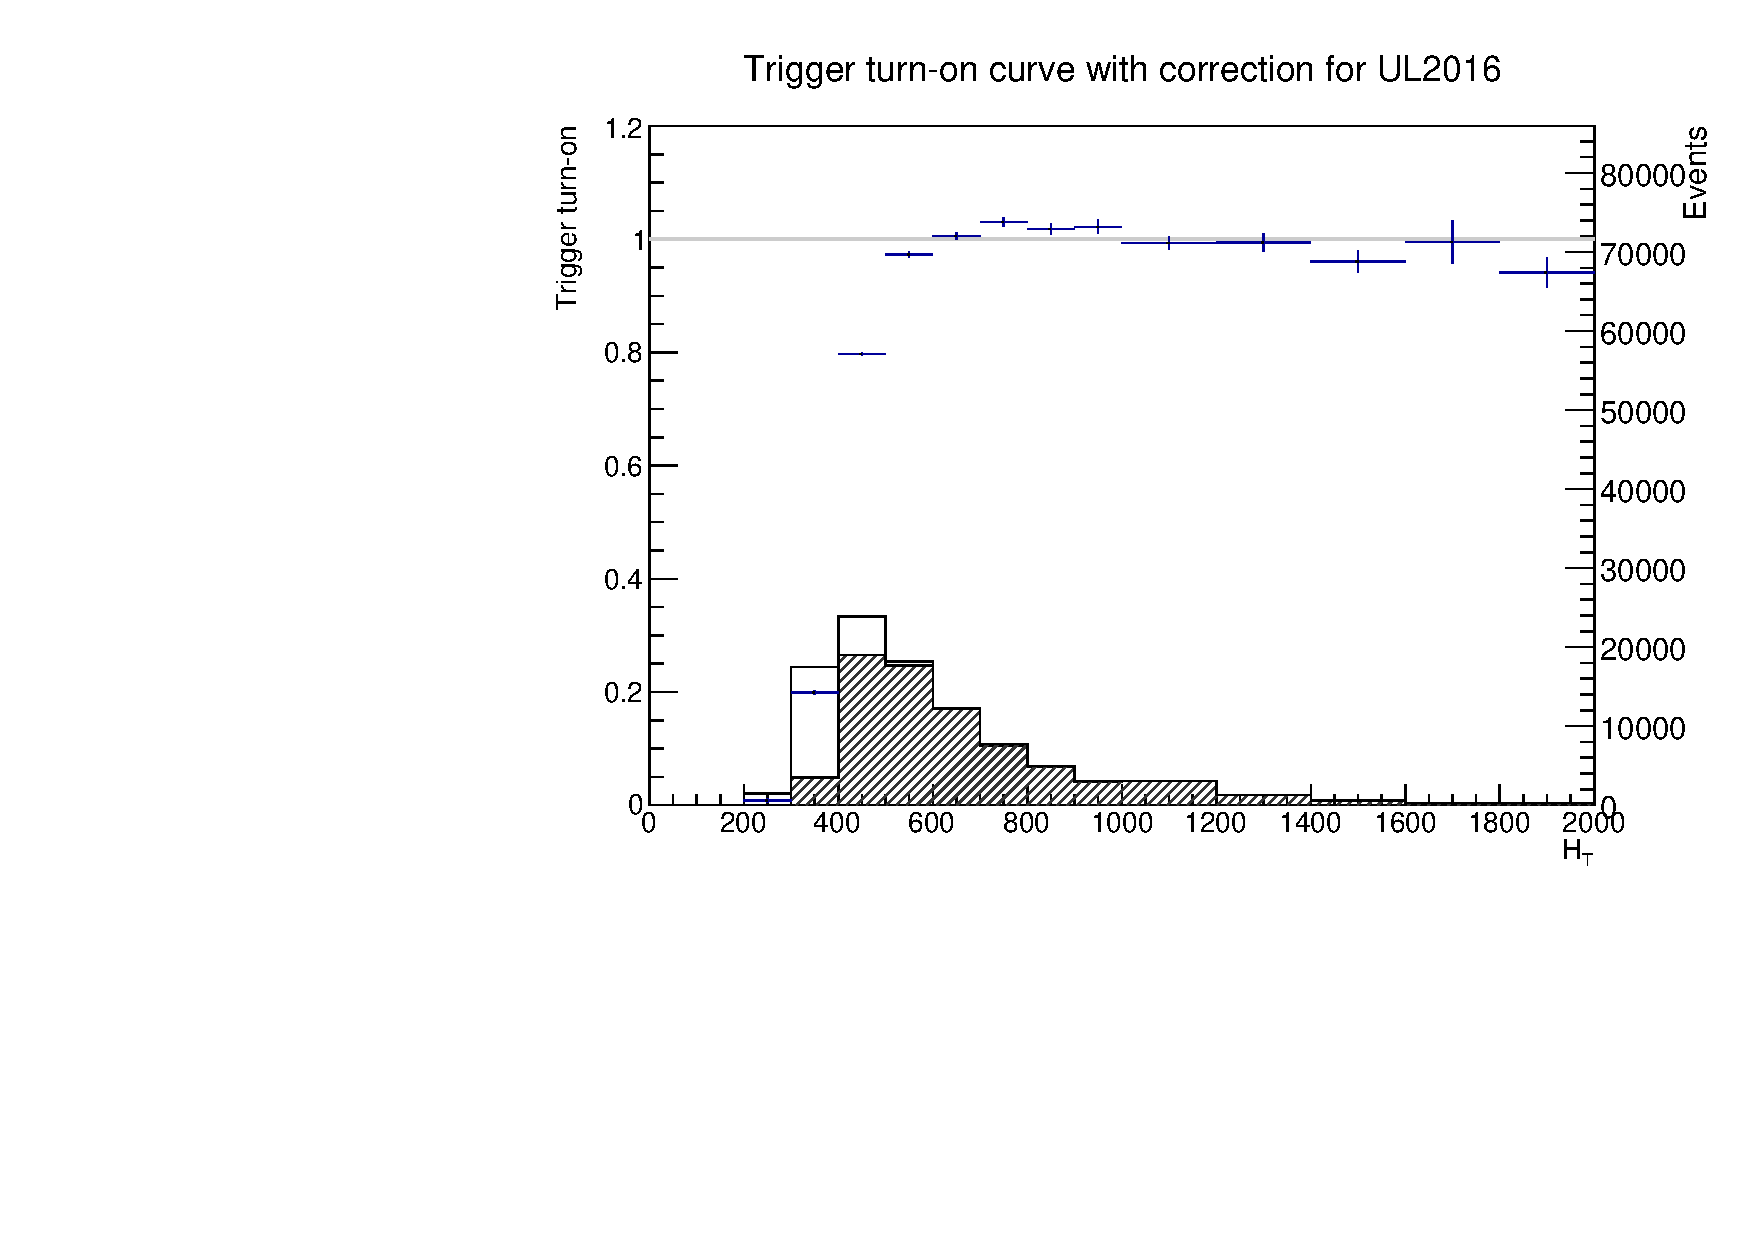
\includegraphics[width=.24\columnwidth]{plots/Trigger/turnOn_UL2016_Coron.pdf}
    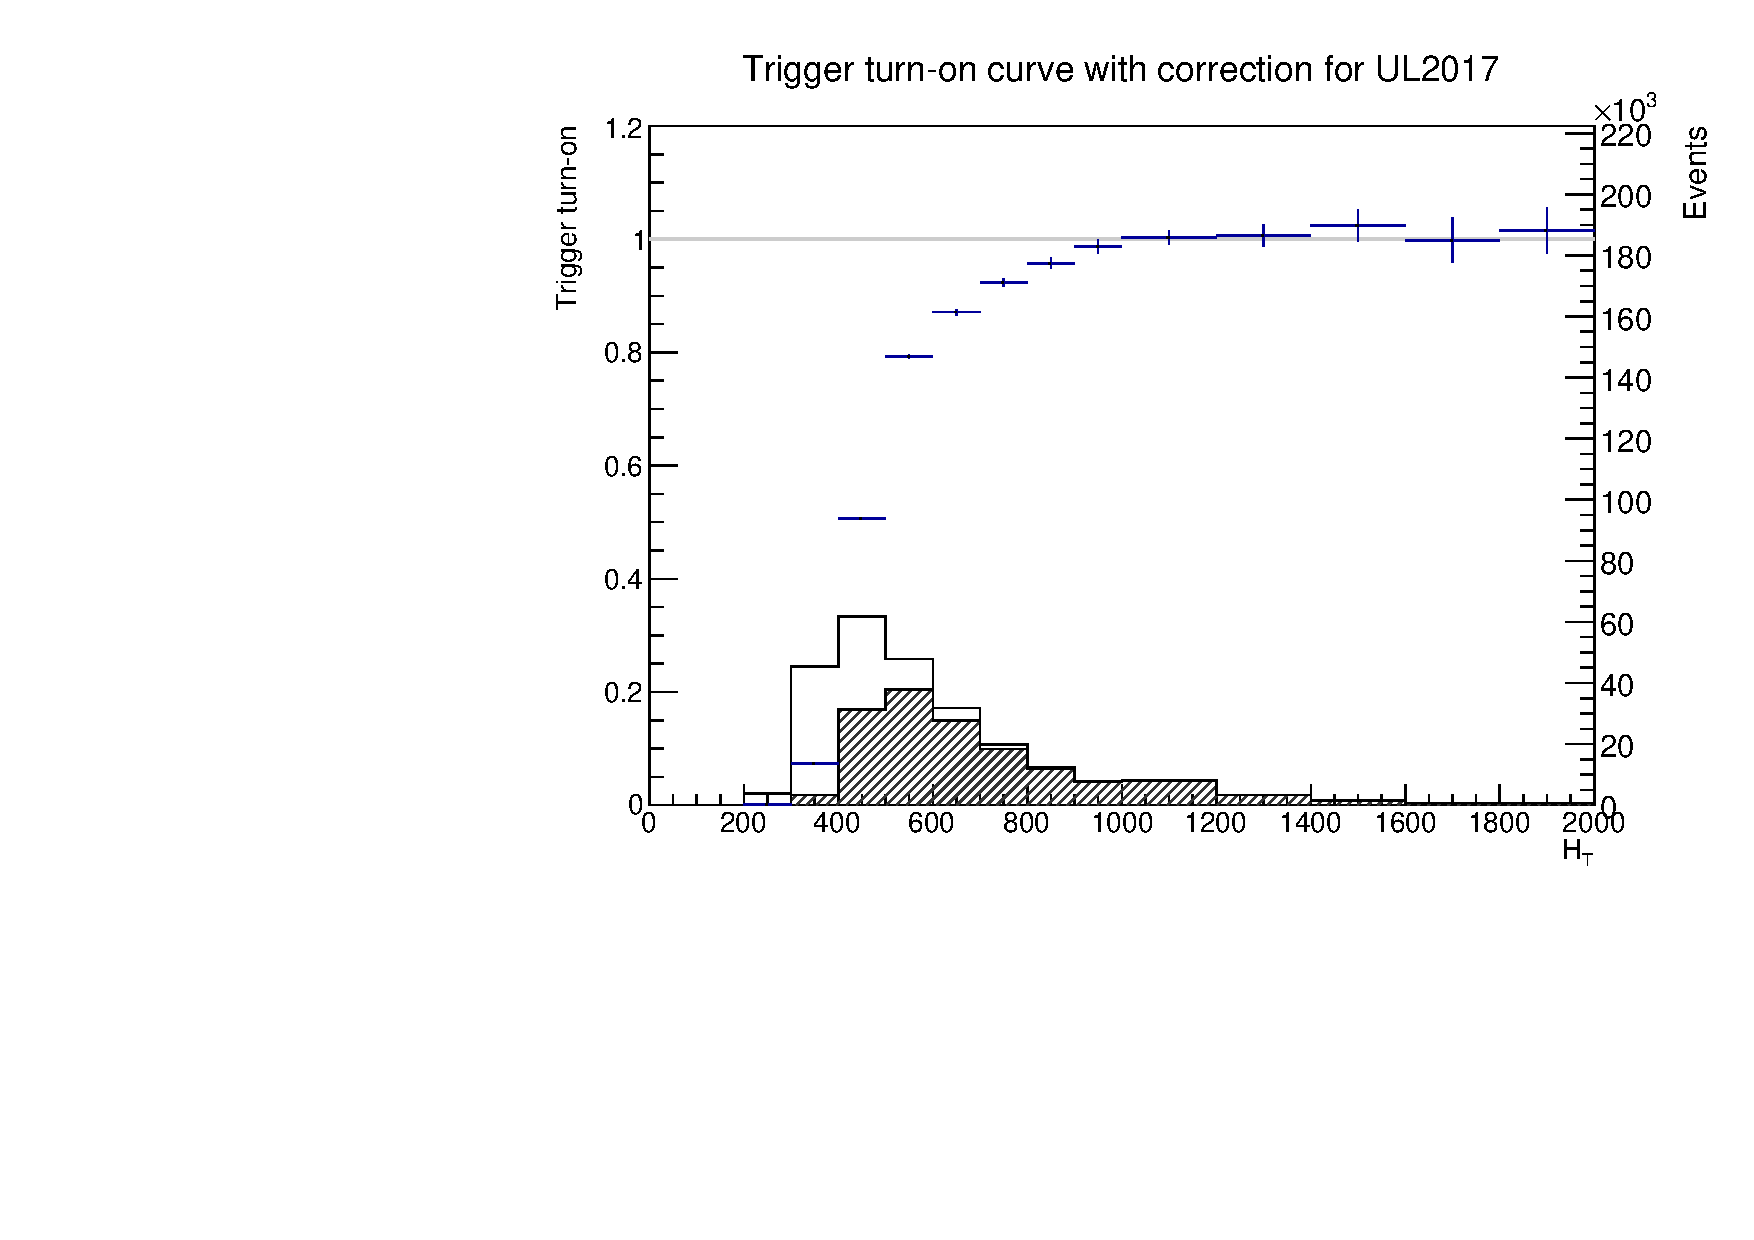
\includegraphics[width=.24\columnwidth]{plots/Trigger/turnOn_UL2017_Coron.pdf}
    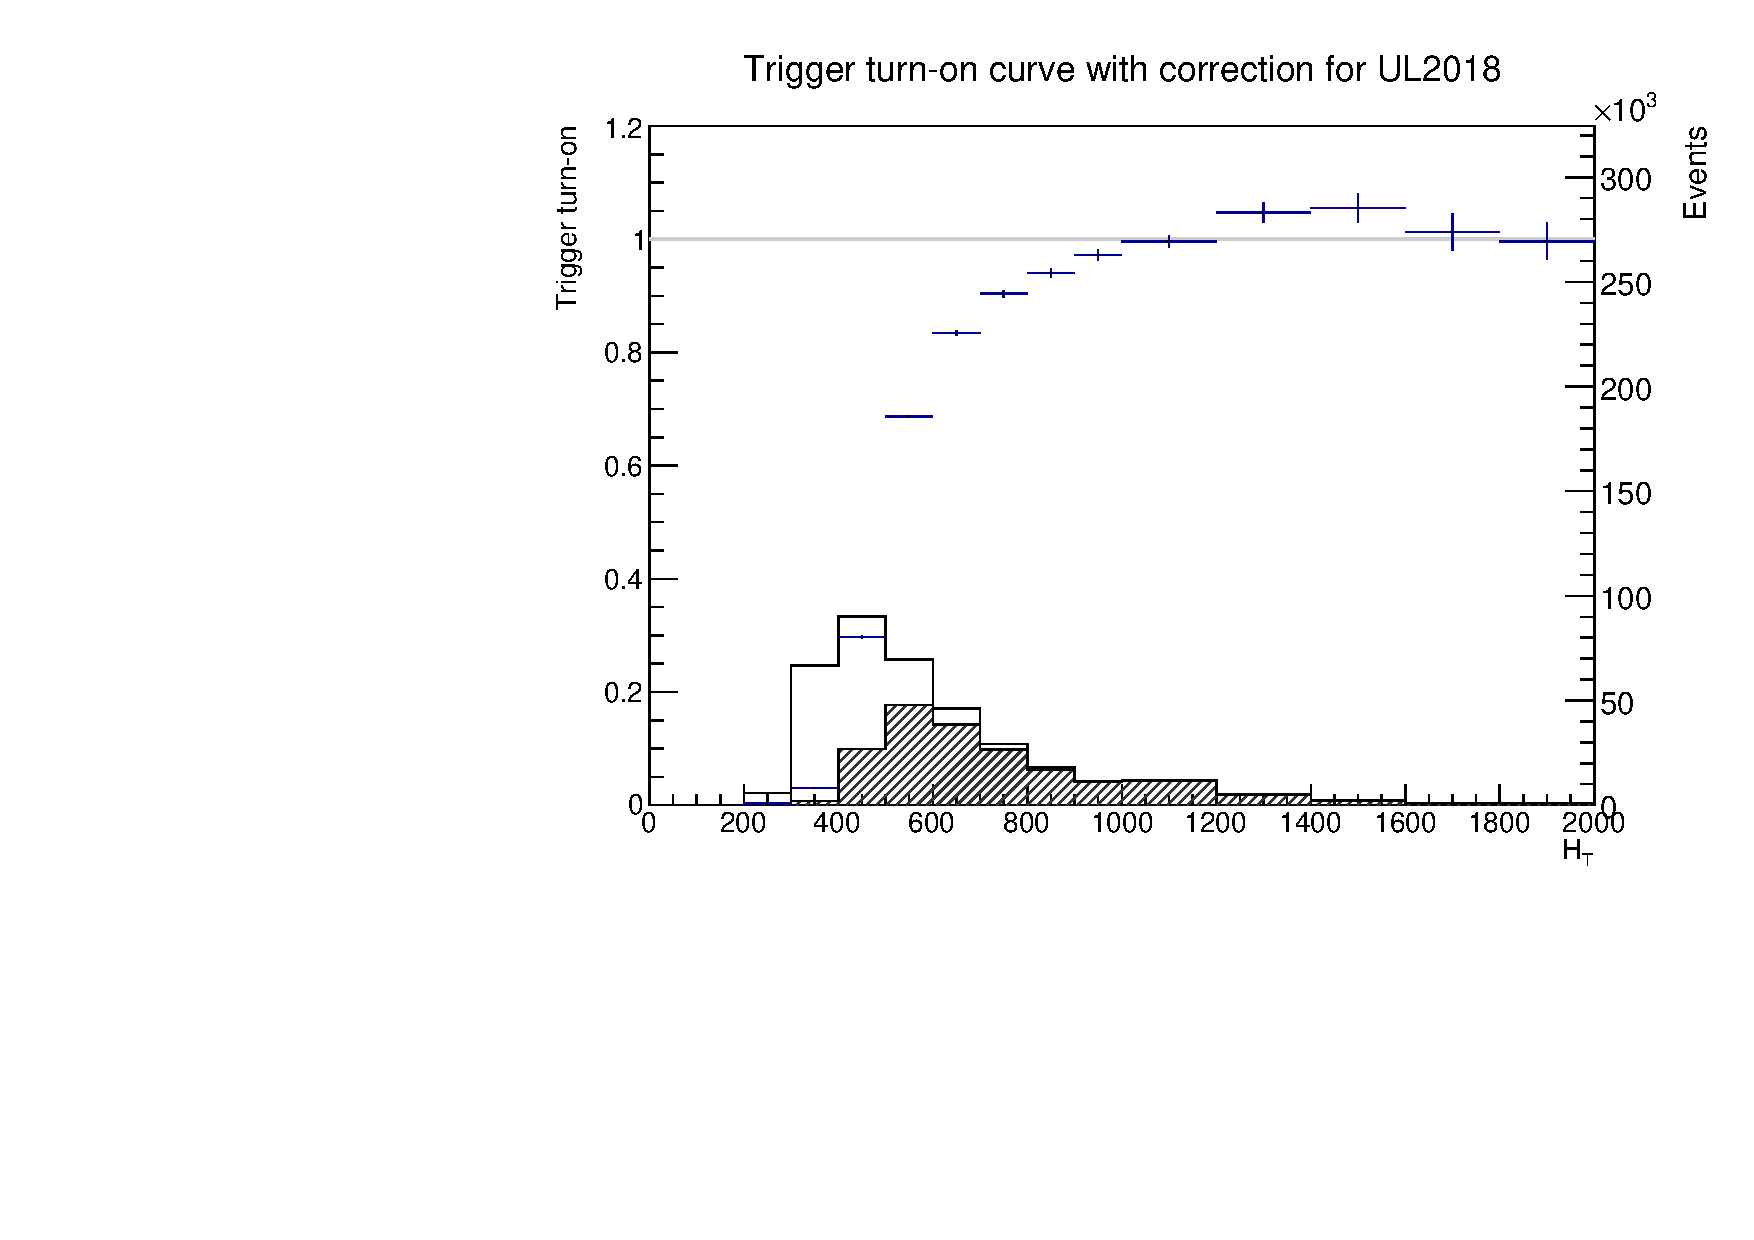
\includegraphics[width=.24\columnwidth]{plots/Trigger/turnOn_UL2018_Coron.pdf}

    
    \caption{Trigger turn-on vs $H_T$ before (top) and after (bottom) correcting for efficiencies measured as a function of $N_{jet}$ and $N_{b-jet}$ for 2016 pre VFP, 2016 post VFP, 2017 and 2018 data.}
    \label{figure_1} 
\end{figure}
\begin{figure}[!t]
    \centering
    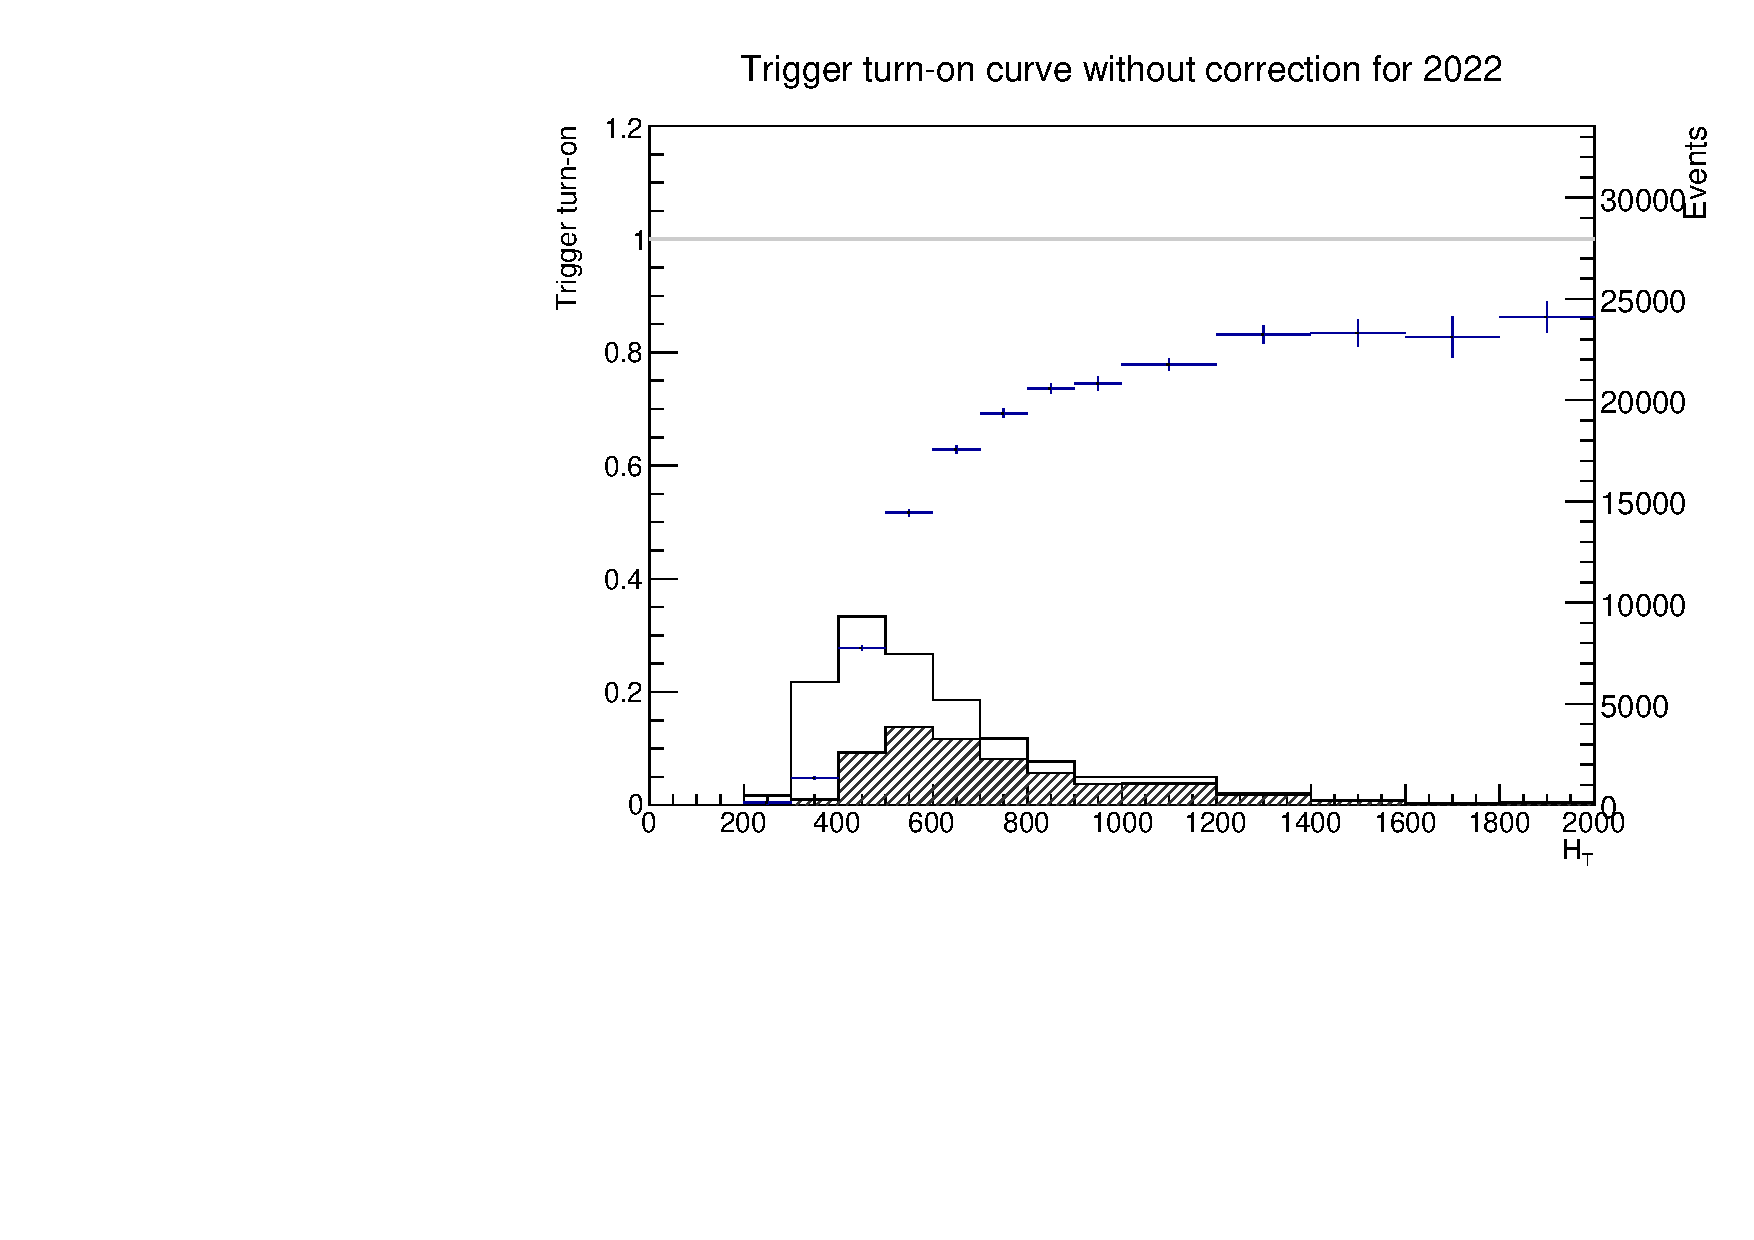
\includegraphics[width=.24\columnwidth]{plots/Trigger/turnOn_2022_Coroff.pdf}
    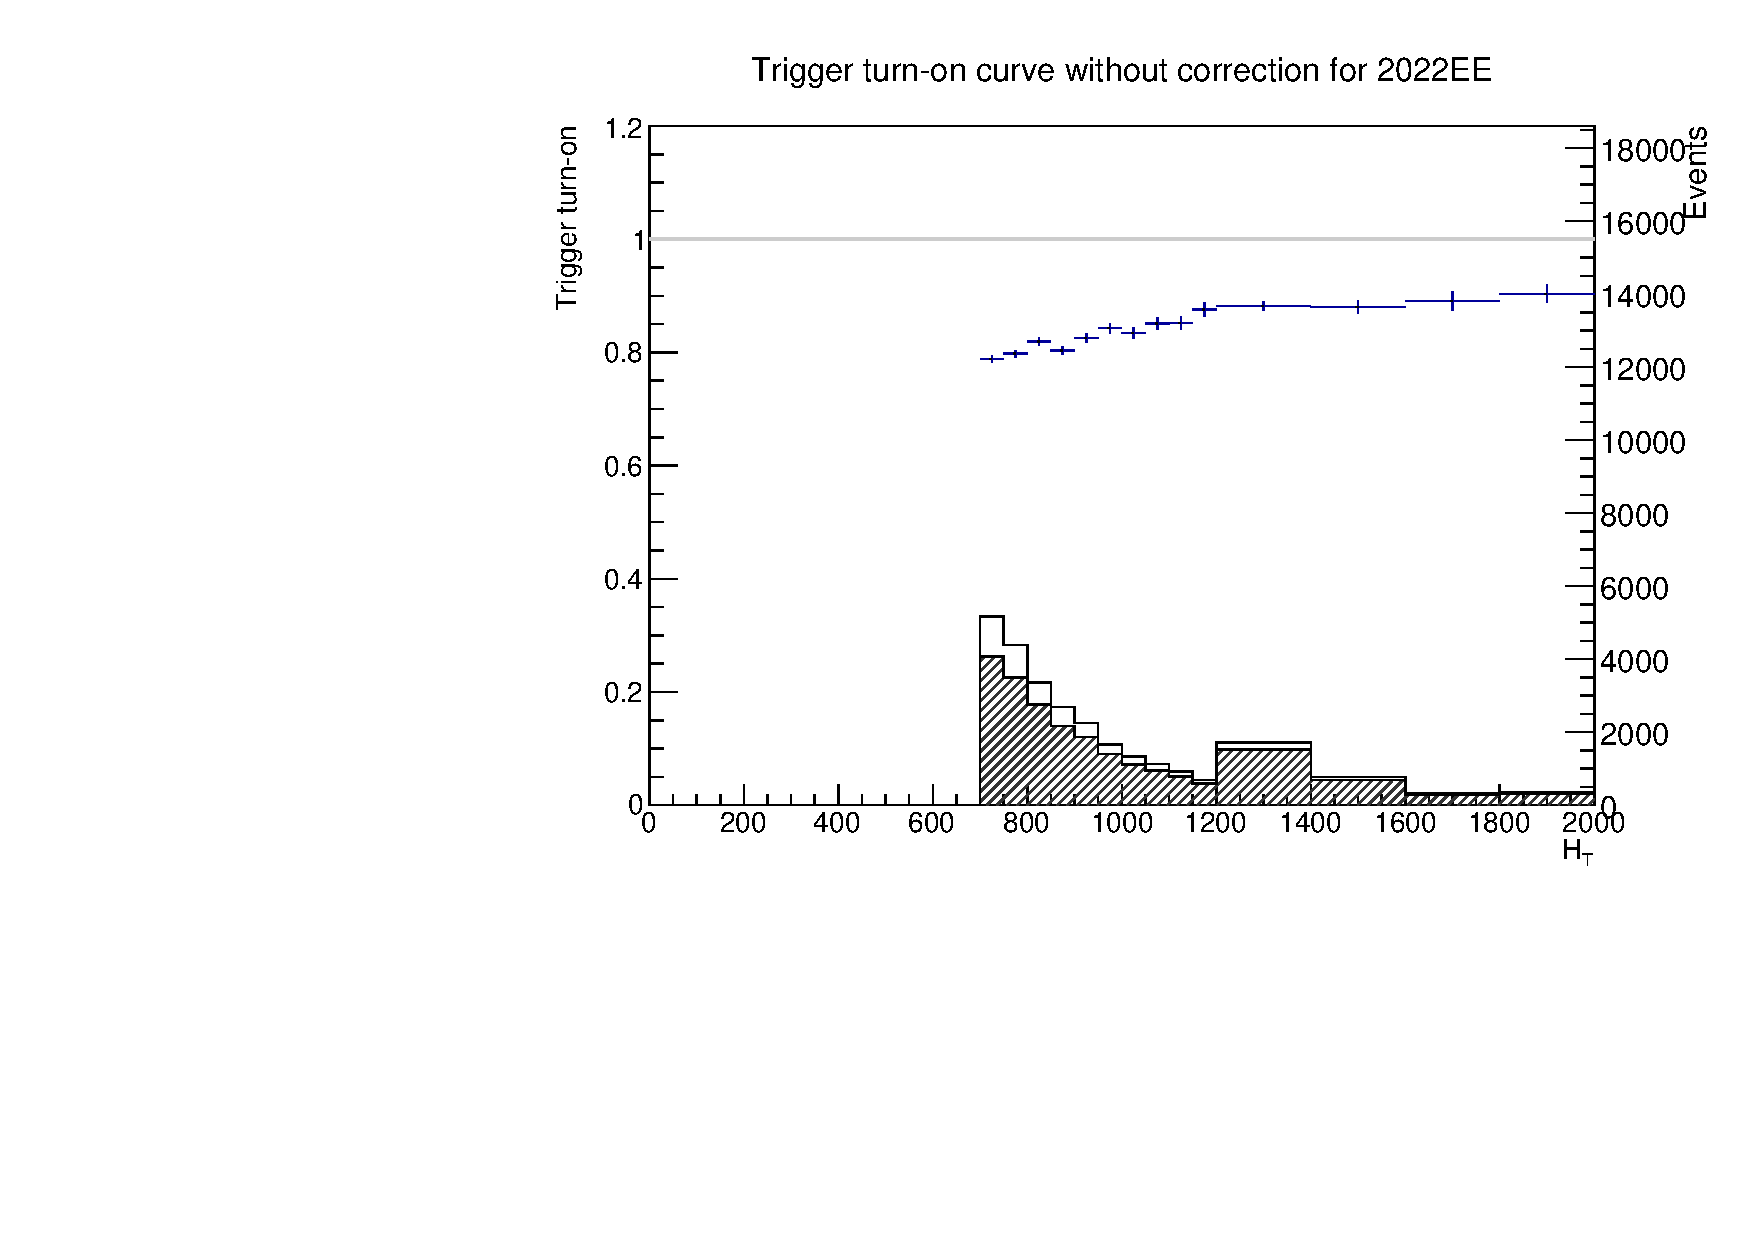
\includegraphics[width=.24\columnwidth]{plots/Trigger/turnOn_2022EE_Coroff.pdf}
    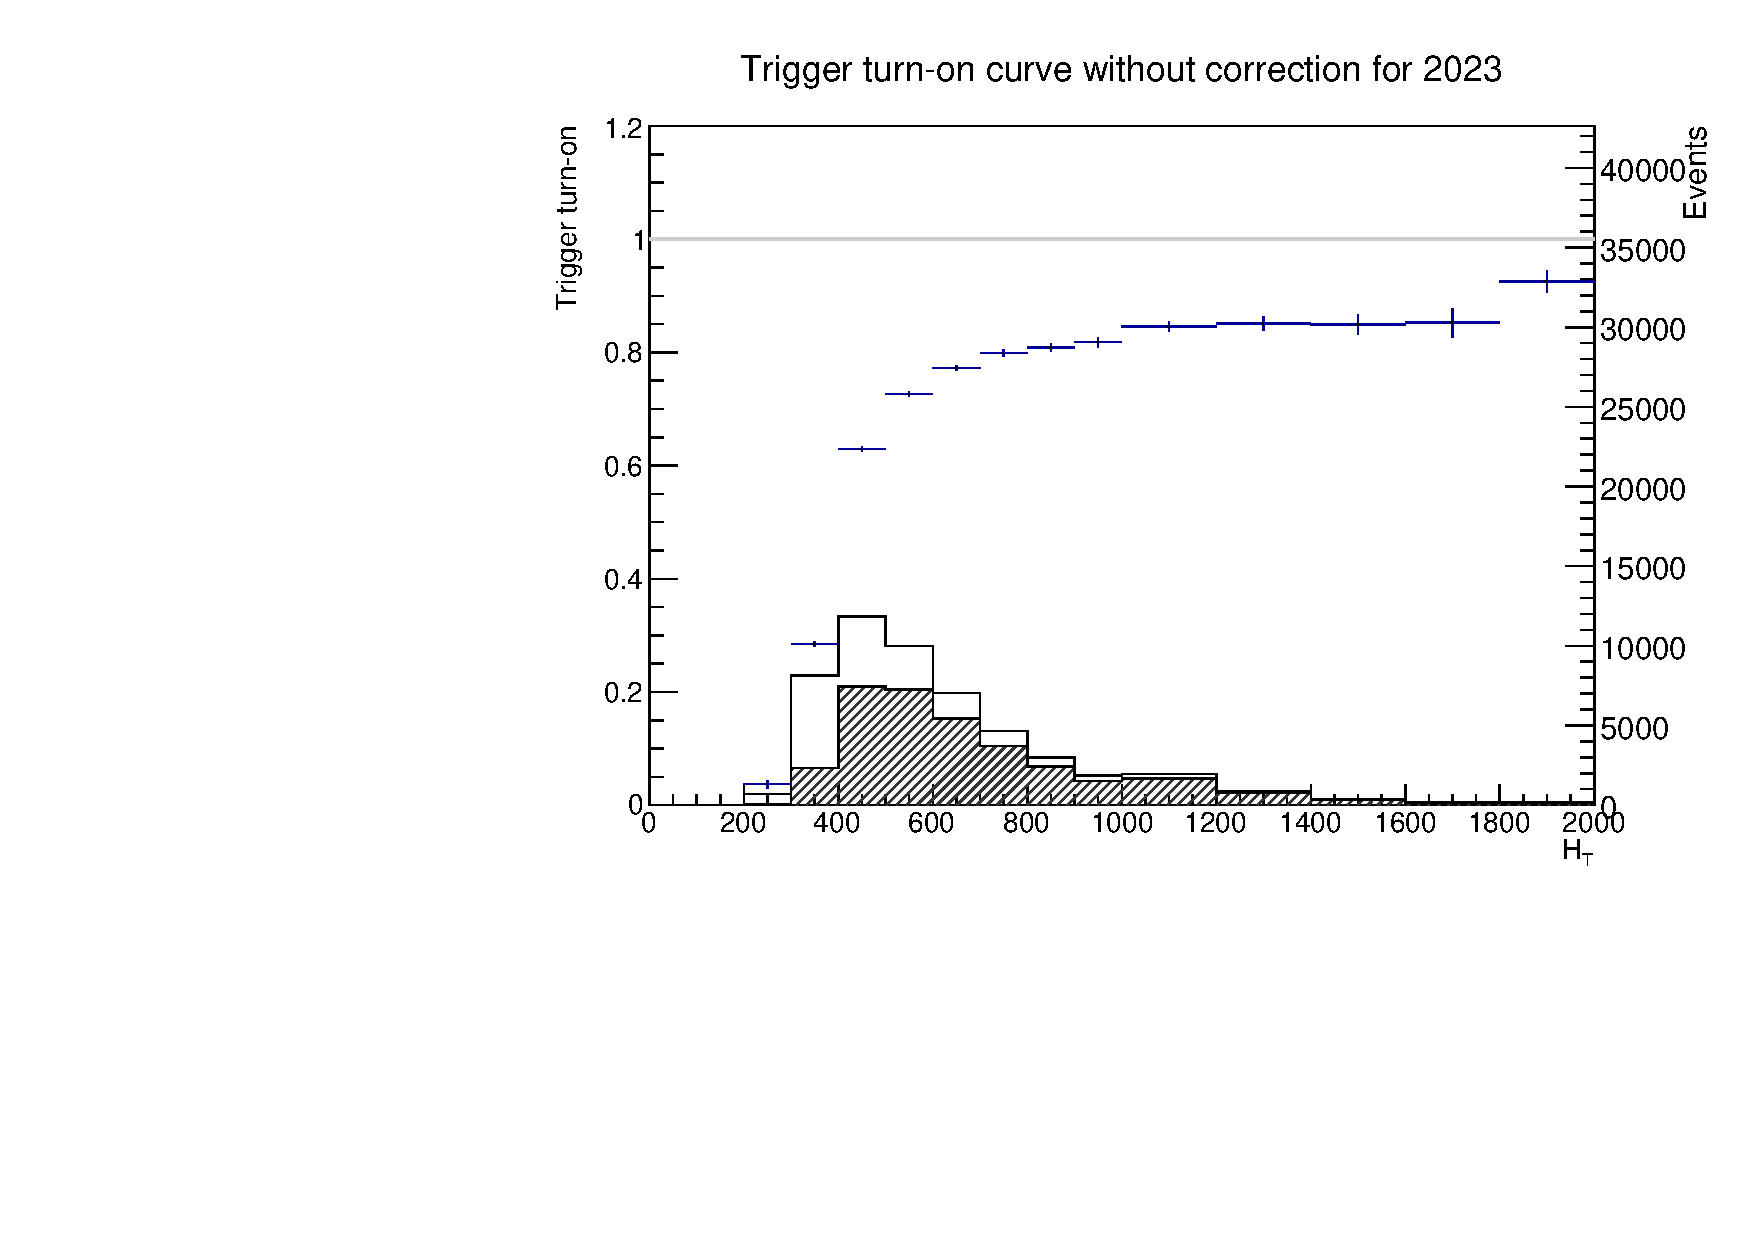
\includegraphics[width=.24\columnwidth]{plots/Trigger/turnOn_2023_Coroff.pdf}
    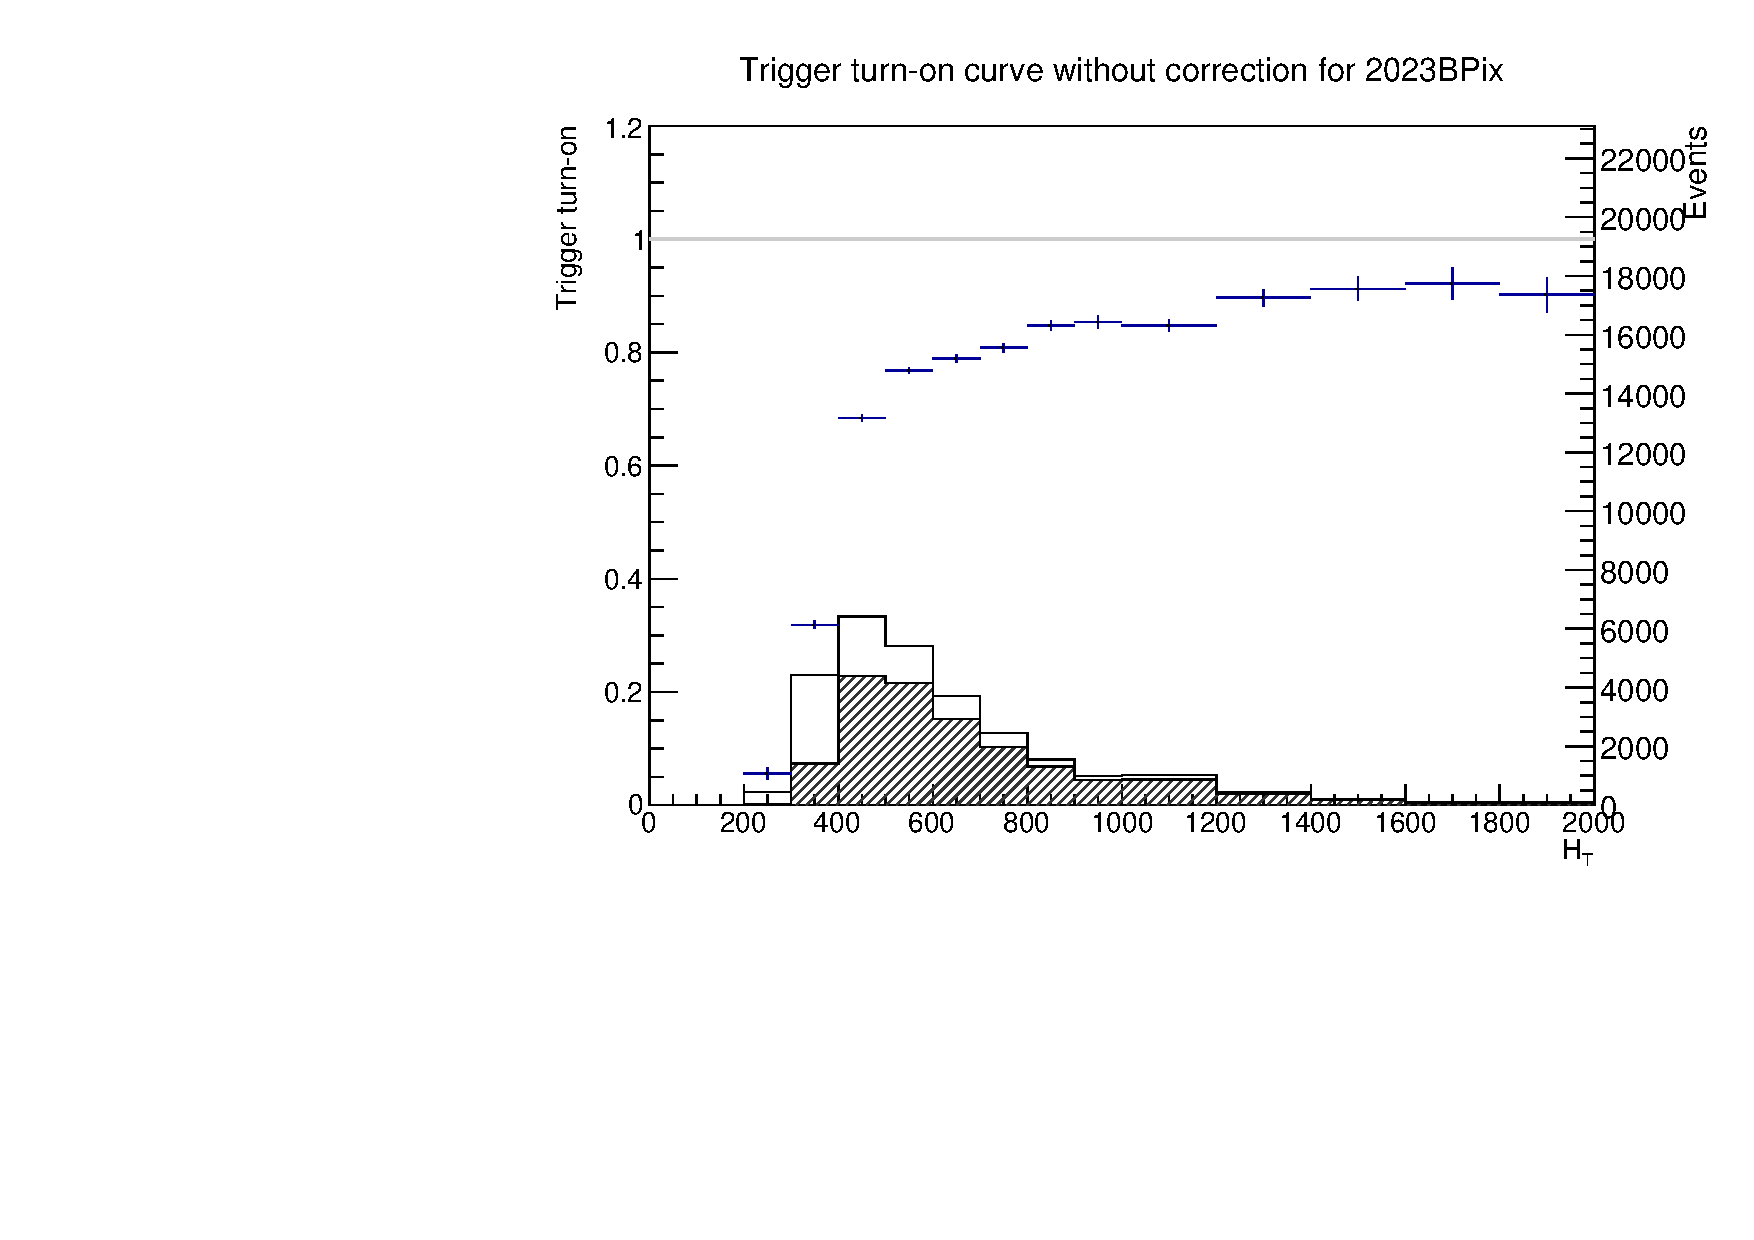
\includegraphics[width=.24\columnwidth]{plots/Trigger/turnOn_2023BPix_Coroff.pdf}
    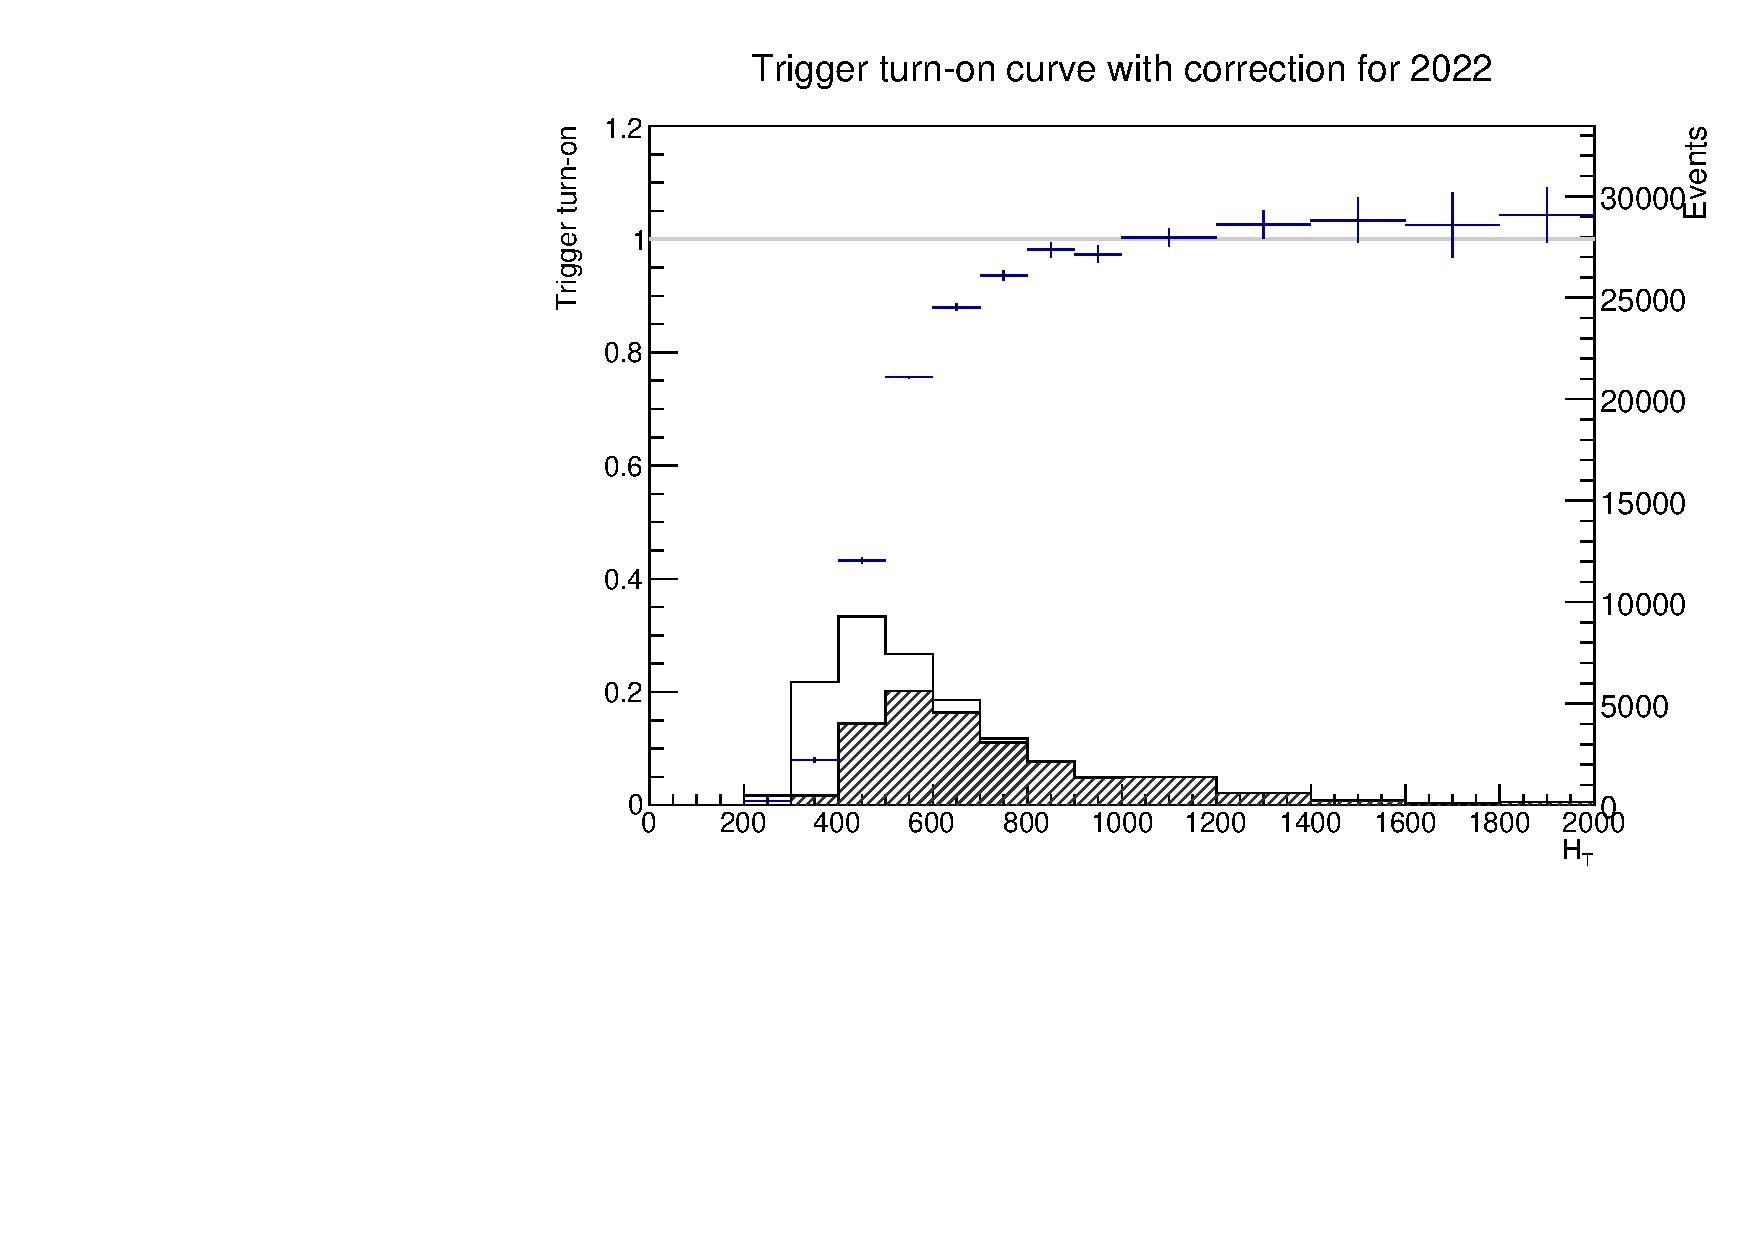
\includegraphics[width=.24\columnwidth]{plots/Trigger/turnOn_2022_Coron.pdf}
    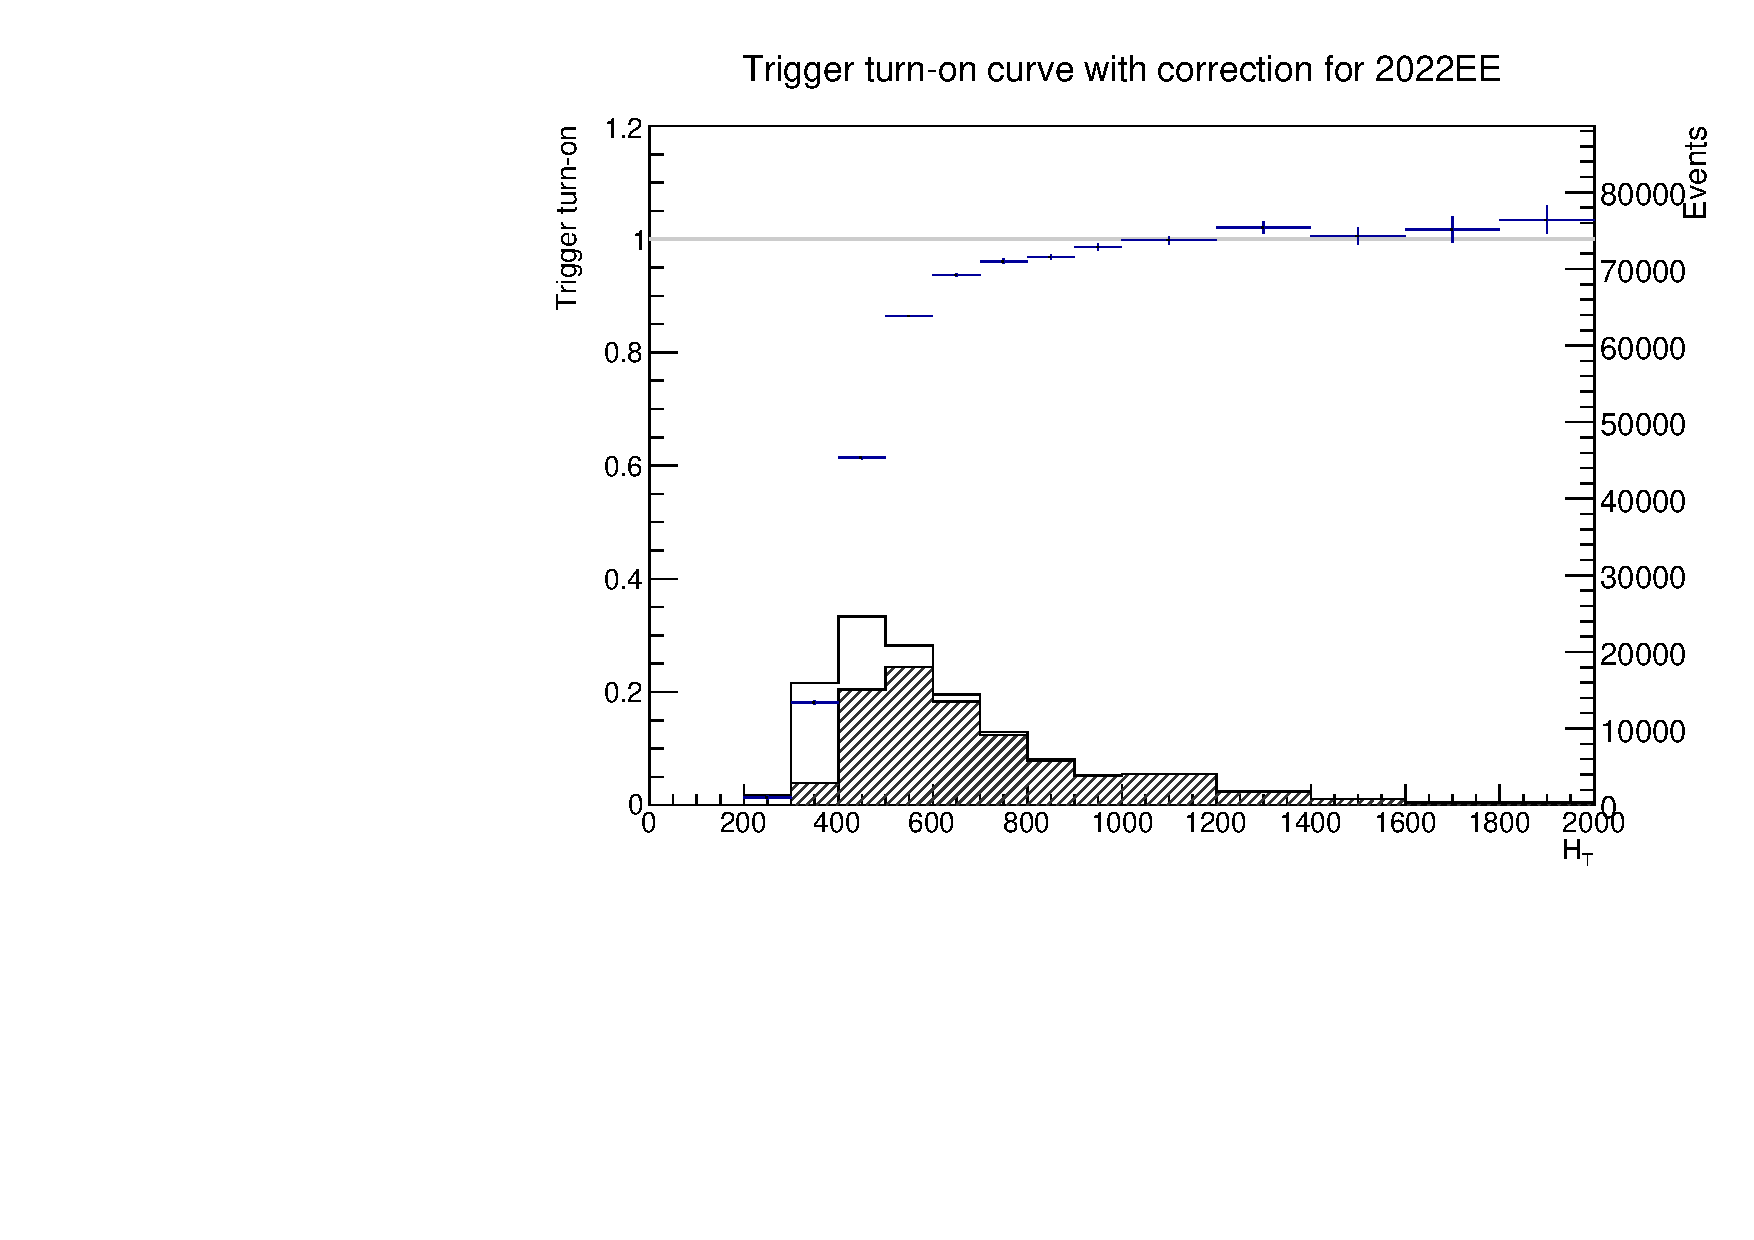
\includegraphics[width=.24\columnwidth]{plots/Trigger/turnOn_2022EE_Coron.pdf}
    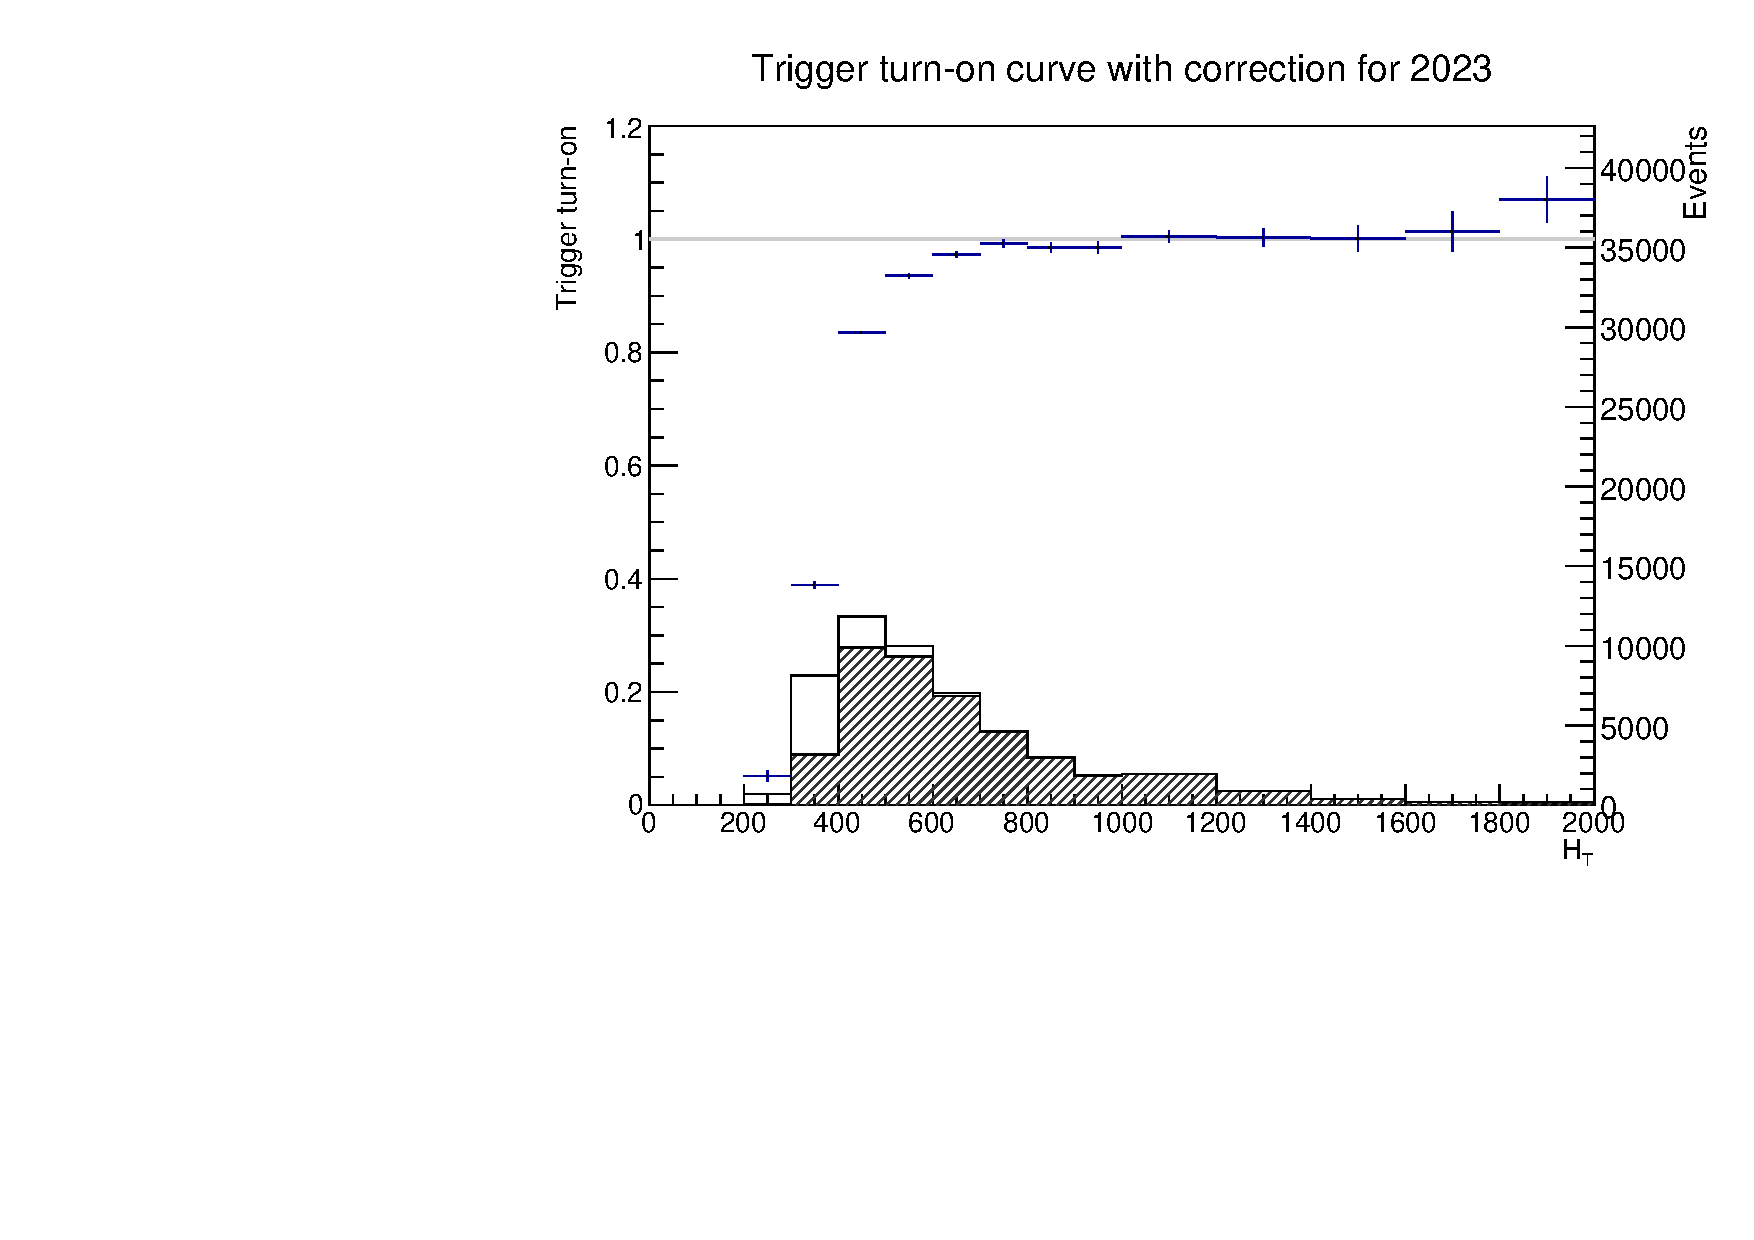
\includegraphics[width=.24\columnwidth]{plots/Trigger/turnOn_2023_Coron.pdf}
    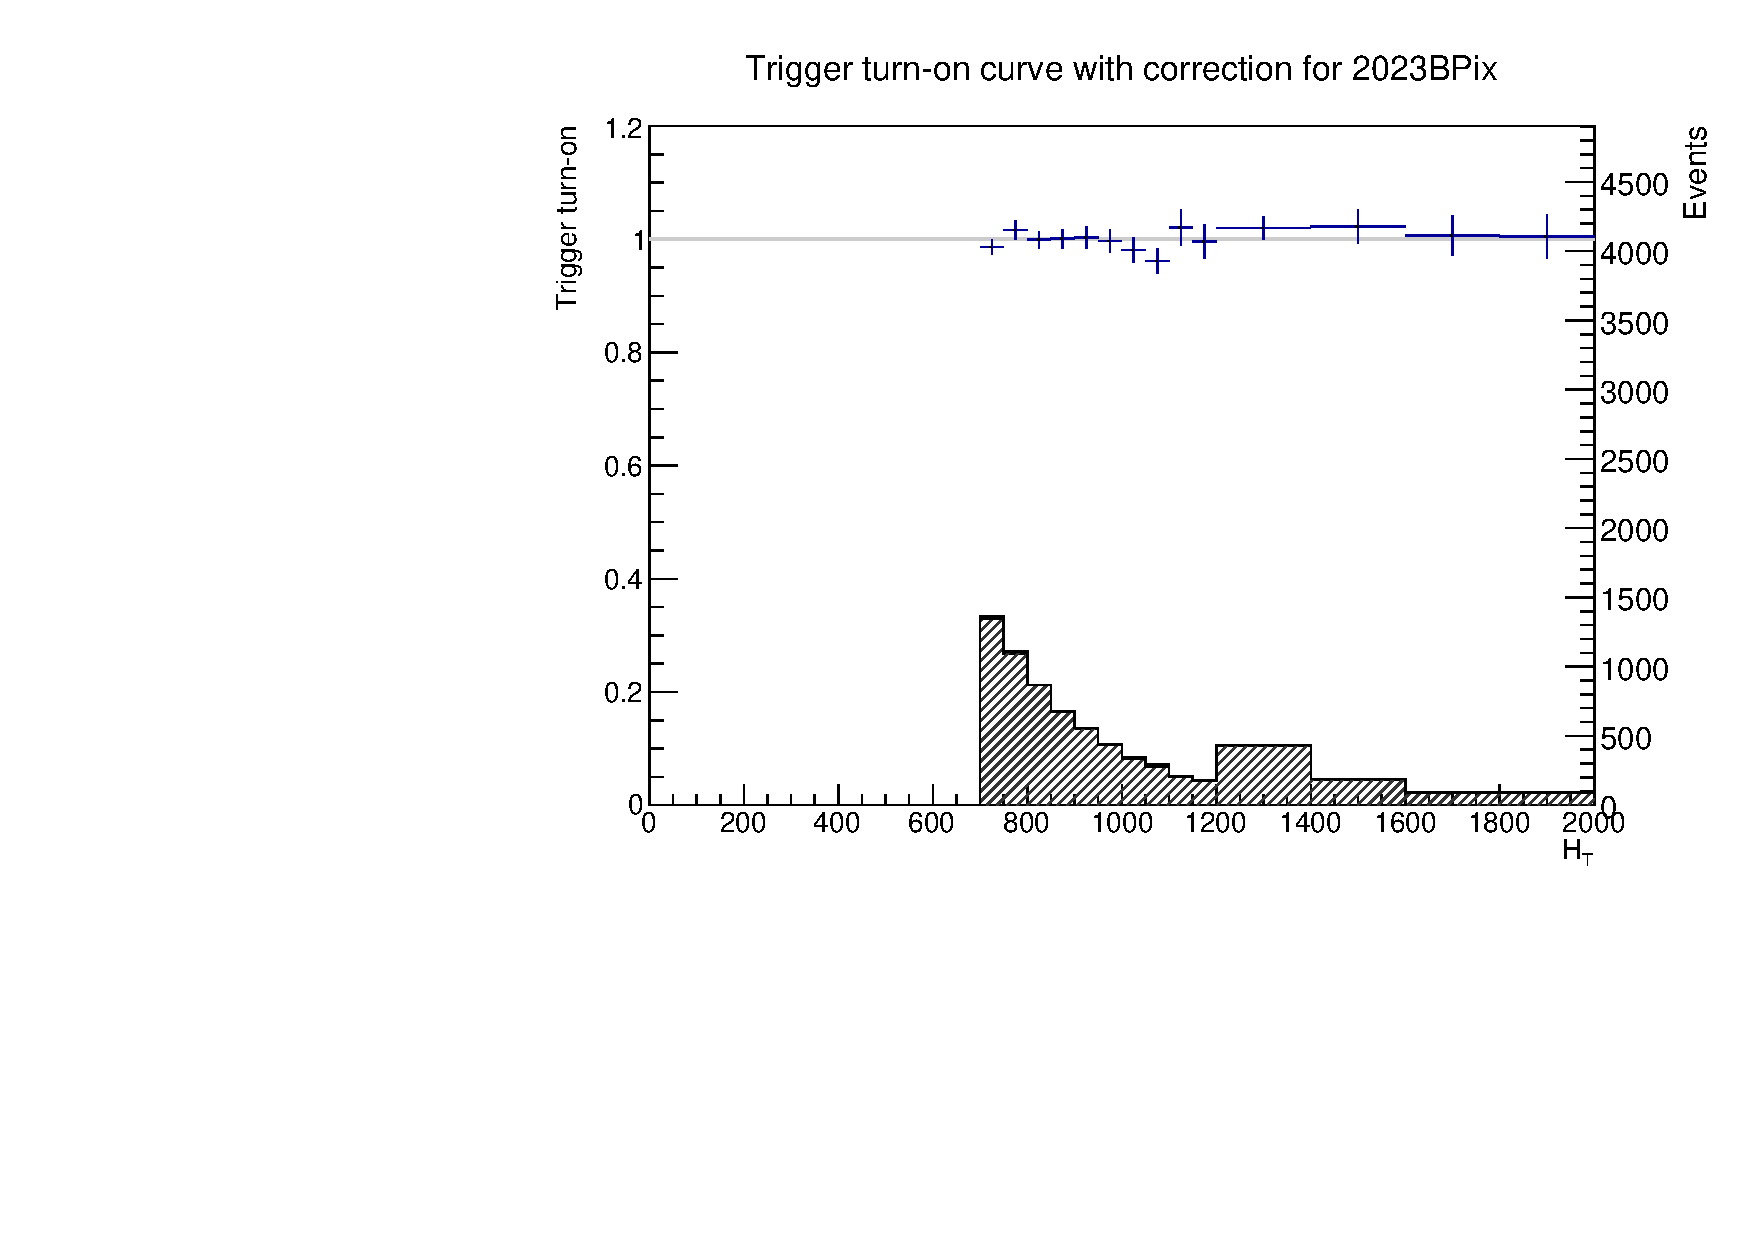
\includegraphics[width=.24\columnwidth]{plots/Trigger/turnOn_2023BPix_Coron.pdf}

    \caption{Trigger turn-on vs $H_T$ for 2022 and 2023 data. Upper plot shows }
    \label{figure_1} 
\end{figure}

The trigger paths include selection criteria based on $N_{jet}$, $N_{b-jet}$, and $H_{T}$. Ideally, the trigger efficiency should be measured as a function of all three variables. However, due to limited statistical precision, the efficiency is measured as a function of $N_{jet}$ and $N_{b-jet}$. To validate that this approach is sufficient, the trigger turn-on curve is used. Figure 3 and 4 show the $H_T$ turn-on for each year before and after applying the $N_{jet}$ and $N_{b-jet}$ dependent corrections. Before the corrections, the efficiency in the plateau region ($H_T \geq 900$ GeV) deviates from unity. After the corrections are applied, the plateau region is close to 1. This behavior shows that the chosen approach is sufficient for measuring the trigger efficiency. The measured trigger efficiency is directly used as trigger SF to MC because the trigger efficiency in not applied at MC in this analysis.

\clearpage
\section{Object Selection}
\label{sec:obj}
\subsection{Vertex Selection}
Standard CMS vertex selection criteria corresponding to the ``goodVertices" flag in NanoAOD is applied. Specifically, each event is required to have at least one primary vertex that satisfies the following criteria:
\begin{itemize}
  \item The vertex must contain trajectories of reconstructed particle tracks with positive $\chi^{2}$ values.
  \item There are at least 5 degrees of freedom in the vertex fit.
  \item The distance, $\left| z \right|$ , along the beam line from the nominal center of the detector is less than 24 cm.
  \item The transverse displacement, r , from the beam line is less than 2 cm.

\end{itemize}

\subsection{Leptons}
\label{sec:leptons}
Events with electron or muon candidates identified with the following criteria are vetoed from the analysis. For the selection of electrons, the EGamma POG ``Fall17-noIso-v2" MVA with a ``loose" working point is used for Run 2. The EGamma ``Winter22V1" MVA noIso score is used for Run 3, with a working point that gives similar signal and background efficiencies as Run 2. We further require that the electrons have $p_T > 15 GeV$ and $\left| \eta \right| < 2.5$, excluding those in the barrel-endcap transition region. The ``loose" muon ID recommended by the Muon POG is used to select muon candidates with $p_T > 15 GeV$ and $\left| \eta \right| < 2.5$. To isolate lepton candidates from hadronic activity, we require the ``mini-isolation" of electrons to be less than 0.4 and ``miniIsoId" for muons to be ``loose".
\subsection{Jets}
Particle Flow jets clustered with the anti-$k_T$ algorithm with distance parameter R = 0.4. To correct for pileup, charged hadron subraction procedure is used for Run 2, where as PUPPI jets are used for Run 3. Latest jet energy corrections as recommended by the JetMET POG is reapplied to recalibrate from the NanoAoD values. The jets are further required to have $p_T > 35 GeV$ and $\left| \eta \right| <2.4$. Additionally, selected jets are required to pass ``tight" working point of Jet ID as recommended by the JetMET POG.

\subsubsection{B-tagging}

B jets are identified with the DeepJet algorithm with the ``M'' working point as recommended by the BTV POG, which corresponds to a b jet efficiency of about 80\%. B tag SF corrections as recommended by the BTV POG is applied.

\subsubsection{W and Boosted Top tagging}

For boosted top quarks with $p_T > 400$GeV, or W bosons with $p_T > 200$GeV, the decay products are expected to be contained within a $\Delta R $ of 0.8. We apply Particlenet algorithm to jets clustered with anti-$k_T$ algorithm with a distance parameter of 0.8 to identify these W and boosted top quarks. Working point corresponding to a 1\% mistag rate as recommended by the JetMET POG is used.  

\subsubsection{Resolved Top tagging}
\label{sec:restop}

For moderately boosted top quarks, the decay products can be resolved into separate AK4 jets. A dedicated XGBoost BDT trigger is developed for tagging these resolved tops, following the same methodology as the Run2 all-hadronic TTTT analysis \cite{prev_analysis}. From the AK4 jets collection, up to four jets with the highest Deepjet b-tag scores are selected. For each b jet candidate, we identify all the unique two-jet combinations in the AK4 jets collection (excluding the b jet candidate) as  W subjet candidates, with the condition that the combined mass of the two W subjet candidate is within 40 GeV of the true W boson mass, and that the mass of the combined three-jet candidate is within 80 GeV of the true top quark mass. These selected three-jet combinations are the candidates for resolved tops. 

The following variables form the inputs to the BDT:

\begin{itemize}
  \item Mass of the b jet candidate
  \item Pairwise invariant mass of the b jet candidate with the W subjet candidate
  \item Mass of the resolved top candidate, from combining the four-vectors of the constituent jets
  \item Combined mass of the two W subjet candidates, from combining the four-vectors of the two W subjet candidates
  \item The product of the top candidate $p_{T}$ and $\Delta R$ between the b jet and the W candidate.
  \item The product of the W candidate $p_{T}$ and $\Delta R$ between the W subjet candidates.
  \item The ``soft-drop condition'' from the soft-drop declustering algorithm reinterpreted as a variable over the two W subjets:$\frac{\min(p_{T1}, p_{T2})}{p_{T1} + p_{T2}} \Delta R_{j_1, j_2}^{-2}$, which tends to reject relatively soft collinear jets.
  \item The DeepJet b-tag scores of all three constituent jets.
  \item The DeepJet c-tag scores of the W subjets. %The c-tag scores is recovered from NanoAOD as $\frac{DeepJet CvsB score * DeepJet B score}{(1.0 -DeepJet CvsB score)}$ according to \cite{btv-20-001}
  \item The quark-gluon likelihood scores of the W subjets. (Run2 Only)
  \item The DeepJet g vs uds discriminator scores of the W subjets. (Run3 Only)
  \item The jet constituent multiplicities of the W subjets.
\end{itemize}

For training, genuine hadronic top candidates are taken from single-lepton $t\bar{t}$ simulation samples, and fake hadronic top candidates from di-lepton $t\bar{t}$ simulation samples, with the requirement of $MET>100$,  $N_{jets}>=5$ and $N_{bjets}>=1$. 2018 samples are used for Run2 model and 2022 samples for Run3. The BDT is trained with the XGBoost library on 500000 candidates for genuine and fake samples each. Before training, to decorrelate from $p_{T}$ of the top candidate, the candidates are reweighted according to the $p_{T}$ of the top candidate in bins of 25 GeV width from 0 Gev to 900 GeV, 50 GeV width from 900 GeV to 1000 GeV, and 100 GeV width from 1000 GeV to 5000 GeV, such that the sum of weights of candidates in each bin is equal. If the resolved top candidates overlap with one another within a $\Delta R$ of 0.4, the lower scoring candidate is rejected.

The working point for this resolved top tagger is selected at 2\% False Positive Rate and given in Table \ref{tab:topWP}.


\begin{table}[h]
\centering
\begin{tabular}{|c|c|}
\hline
\textbf{Year} & \textbf{topWP} \\ 
\hline
2016preVFP  & 0.961  \\
2016     & 0.954  \\
2017     & 0.961  \\
2018     & 0.961  \\
2022     & 0.966 \\
2022EE   & 0.968  \\
2023     & 0.963  \\
2023BPix & 0.969 \\
\hline
\end{tabular}
\caption{Resolved TopWP values for different years}
\label{tab:topWP}
\end{table}

Scales factors for tagging efficiencies and misidentification rates are derived for this resolved top tagger. These scale factors are parameterized in the resolved top candidate $p_{T}$, and the uncertainties thereof are propagated as part of the systematic uncertainties. For scale factor derivations, b-tag SF corrections, pileup weight and latest JERC corrections is applied to MC samples in the following procedure.

For the derivation of the misidentification rates, we use a 0-lepton, $N_{b}=1$ region, selected with pure $H_{T}$ triggers and requiring $H_{T}>1200 GeV$. This region was selected to be enriched in QCD multi-jet events and is orthogonal to the signal region via the $N_{b}=1$ requirement. In this region, simulation is normalized to data. To correct the contamination of genuine tops in the data, we estimate the number of genuine tops in data by the number of candidates matched to top quarks at the generator level in simulation, and then subtract it from the data. In simulation, the misidentification rates are measured to be the fraction of fake resolved top candidates that pass the working point. In data, the misidentification rates are measured to be the fraction of candidates (after subtraction of the estimated genuine tops) that pass the working point. In the end, the scale factor is calculated as the ratio of the misidentification rates in data to those in simulation.

For the derivation of the tagging efficiency scale factor, we used single muon triggers to define a control region selected to be enriched in semi-leptonic $t\bar{t}$ events with similar kinematics to the Signal Region. This region is orthogonal to the Signal Region via the requirement on the muon. We further require that the events to be $N_b \geq 2, N_j \geq 4, p_T^{\text{miss}} > 75\, \text{GeV}$, and muon $ p_T > 50\, \text{GeV}.$ In each event, jets are first cleaned against leptons, and resolved top candidates cleaned against muons with a $\Delta R$ of 0.4. We first normalize simulation to data. The misidentification scale factor is applied to candidates in simulation that pass the working point but fail to be matched to top quarks at generator level. Candidates are then split into three $p_T$ categories: low ($100-300GeV$), medium ($300-500GeV$) and high ($\ge500GeV$). We then perform a simultaneous template fit, where two templates of candidates in simulation matched and unmatched to top quarks at generator level respectively are used. The templates are binned in top candidate mass, since it is independent of candidate $p_T$. The fit from simulation to data is performed simultaneously for candidates passing and failing the working point. In each $p_T$ category, the tagging efficiency scale factor is calculated as $\frac{\epsilon_{post-fit}}{\epsilon_{pre-fit}}$, where tagging efficiency $\epsilon$ is defined as the ratio of number of matched (genuine) top candidates passing the working point to the total number of matched top candidates, and $\epsilon_{post-fit}$ is the tagging efficiency in data estimated from fitting simulation to data.

\begin{figure}[H]
\centering
% Grid for _mistag images
%\noindent % Remove indentation
%\newcounter{rowcounter} % Create the rowcounter for managing rows
\setcounter{rowcounter}{0} % Initialize the rowcounter
\foreach \key in {2016preVFP, 2016, 2017, 2018, 2022, 2022EE, 2023, 2023BPix} {
    \begin{minipage}{0.3\textwidth} % Adjust the width to fit 3 images per row
        %\centering
        \includegraphics[width=\textwidth]{plots/restop_mistag/norm/\key\_mistag.png}
    \end{minipage}
    \ifnum\value{rowcounter}=2
        \par % Move to the next row after every 3 images
        \setcounter{rowcounter}{0} % Reset rowcounter
    \else
        %\hspace{0.03\textwidth} % Add horizontal space between images
        \stepcounter{rowcounter} % Increment rowcounter
    \fi
}
% Caption and label for the Mistag grid
\caption{Distributions of resolved top candidate $p_T$ in data and simulation for all candidates in the region used to derive the misidentification rate scale factor. Contributions from different processes as estimated from simulation are shown in the stacked
histograms. The event yield in simulation is scaled to match data inclusively in this region,
prior to the application of the top tagger working point.}
\label{fig:mistag_norm}
\end{figure}

\begin{figure}[H]
\centering
% Grid for _mistag images
%\noindent % Remove indentation
%\newcounter{rowcounter} % Create the rowcounter for managing rows
\setcounter{rowcounter}{0} % Initialize the rowcounter
\foreach \key in {2016preVFP, 2016, 2017, 2018, 2022, 2022EE, 2023, 2023BPix} {
    \begin{minipage}{0.3\textwidth} % Adjust the width to fit 3 images per row
        %\centering
        \includegraphics[width=\textwidth]{plots/restop_mistag/norm/\key\_passTopWP_mistag.png}
    \end{minipage}
    \ifnum\value{rowcounter}=2
        \par % Move to the next row after every 3 images
        \setcounter{rowcounter}{0} % Reset rowcounter
    \else
        %\hspace{0.03\textwidth} % Add horizontal space between images
        \stepcounter{rowcounter} % Increment rowcounter
    \fi
}
% Caption and label for the Mistag grid
\caption{Distributions of resolved top candidate $p_T$ in data and simulation for candidates passing the working point in the region used to derive the misidentification rate scale factor. Contributions from different processes as estimated from simulation are shown in the stacked histograms. The event yield in simulation is normalized to data by the scale obtained from the same distributions for all candidates in Figure \ref{fig:mistag_norm}}
\label{fig:mistag_passwp_norm}
\end{figure}

\begin{figure}[H]
\centering
% Grid for _mistag images
%\noindent % Remove indentation
%\newcounter{rowcounter} % Create the rowcounter for managing rows
\setcounter{rowcounter}{0} % Initialize the rowcounter
\foreach \key in {2016preVFP, 2016, 2017, 2018, 2022, 2022EE, 2023, 2023BPix} {
    \begin{minipage}{0.3\textwidth} % Adjust the width to fit 3 images per row
        %\centering
        \includegraphics[width=\textwidth]{plots/restop_mistag/genmatch/\key\_mistag_genmatch.png}
    \end{minipage}
    \ifnum\value{rowcounter}=2
        \par % Move to the next row after every 3 images
        \setcounter{rowcounter}{0} % Reset rowcounter
    \else
        %\hspace{0.03\textwidth} % Add horizontal space between images
        \stepcounter{rowcounter} % Increment rowcounter
    \fi
}
% Caption and label for the Mistag grid
\caption{Distributions of resolved top candidate $p_T$ in data and simulation for all candidates in the region used to derive the misidentification rate scale factor. Contributions from candidates matched and not matched to top quarks at the generator level
in simulation are shown in the stacked histograms. The event yield in simulation is scaled to match data inclusively in this region,
prior to the application of the top tagger working point.}
\label{fig:mistag_genmatch}
\end{figure}

\begin{figure}[H]
\centering
% Grid for _mistag images
%\noindent % Remove indentation
%\newcounter{rowcounter} % Create the rowcounter for managing rows
\setcounter{rowcounter}{0} % Initialize the rowcounter
\foreach \key in {2016preVFP, 2016, 2017, 2018, 2022, 2022EE, 2023, 2023BPix} {
    \begin{minipage}{0.3\textwidth} % Adjust the width to fit 3 images per row
        %\centering
        \includegraphics[width=\textwidth]{plots/restop_mistag/genmatch/\key\_passTopWP_mistag_genmatch.png}
    \end{minipage}
    \ifnum\value{rowcounter}=2
        \par % Move to the next row after every 3 images
        \setcounter{rowcounter}{0} % Reset rowcounter
    \else
        %\hspace{0.03\textwidth} % Add horizontal space between images
        \stepcounter{rowcounter} % Increment rowcounter
    \fi
}
% Caption and label for the Mistag grid
\caption{Distributions of resolved top candidate $p_T$ in data and simulation for candidates passing the working point in the region used to derive the misidentification rate scale factor. Contributions from candidates matched and not matched to top quarks at the generator level
in simulation are shown in the stacked histograms. The event yield in simulation is normalized to data by the scale obtained from the same distributions for all candidates in Figure \ref{fig:mistag_norm}}
\label{fig:mistag_passwp_genmatch}
\end{figure}

\begin{figure}[H]
\centering
% Grid for _mistag images
%\noindent % Remove indentation
%\newcounter{rowcounter} % Create the rowcounter for managing rows
\setcounter{rowcounter}{0} % Initialize the rowcounter
\foreach \key in {2016preVFP, 2016, 2017, 2018, 2022, 2022EE, 2023, 2023BPix} {
    \begin{minipage}{0.3\textwidth} % Adjust the width to fit 3 images per row
        %\centering
        \includegraphics[width=\textwidth]{plots/restop_mistag/genmatch/\key\_mistag_SF.png}
        \vspace{0.5em} 
        \text{   \key }
    \end{minipage}
    \ifnum\value{rowcounter}=2
        \par % Move to the next row after every 3 images
        \setcounter{rowcounter}{0} % Reset rowcounter
    \else
        %\hspace{0.03\textwidth} % Add horizontal space between images
        \stepcounter{rowcounter} % Increment rowcounter
    \fi
}
% Caption and label for the Mistag grid
\caption{Misidentification rates measured in data and simulation after subtracting the estimated contribution from genuine tops. Misidentification rate scale factors are defined as the ratio of misidentification rate of data over simulation.}
\label{fig:mistag_sf}
\end{figure}

\begin{figure}[H]
\centering
% Grid for _mistag images
%\noindent % Remove indentation
%\newcounter{rowcounter} % Create the rowcounter for managing rows
\setcounter{rowcounter}{0} % Initialize the rowcounter
\foreach \key in {2016preVFP, 2016, 2017, 2018, 2022, 2022EE} {
    \begin{minipage}{0.3\textwidth} % Adjust the width to fit 3 images per row
        %\centering
        \includegraphics[width=\textwidth]{plots/restop_tageff/norm/\key\_tageff.png}
    \end{minipage}
    \ifnum\value{rowcounter}=2
        \par % Move to the next row after every 3 images
        \setcounter{rowcounter}{0} % Reset rowcounter
    \else
        %\hspace{0.03\textwidth} % Add horizontal space between images
        \stepcounter{rowcounter} % Increment rowcounter
    \fi
}
% Caption and label for the Mistag grid
\caption{Distributions of resolved top candidate $p_T$ in data and simulation for all candidates in the region used to derive the tagging efficiency scale factor. Contributions from different processes as estimated from simulation are shown in the stacked
histograms. The event yield in simulation is scaled to match data inclusively in this region,
prior to the application of the top tagger working point.}
\label{fig:tageff_norm}
\end{figure}

\begin{figure}[H]
\centering
% Grid for _mistag images
%\noindent % Remove indentation
%\newcounter{rowcounter} % Create the rowcounter for managing rows
\setcounter{rowcounter}{0} % Initialize the rowcounter
\foreach \key in {2016preVFP, 2016, 2017, 2018, 2022, 2022EE} {
    \begin{minipage}{0.3\textwidth} % Adjust the width to fit 3 images per row
        %\centering
        \includegraphics[width=\textwidth]{plots/restop_tageff/norm/\key\_passTopWP_tageff.png}
    \end{minipage}
    \ifnum\value{rowcounter}=2
        \par % Move to the next row after every 3 images
        \setcounter{rowcounter}{0} % Reset rowcounter
    \else
        %\hspace{0.03\textwidth} % Add horizontal space between images
        \stepcounter{rowcounter} % Increment rowcounter
    \fi
}
% Caption and label for the Mistag grid
\caption{Distributions of resolved top candidate $p_T$ in data and simulation for candidates passing the working point in the region used to derive the tagging efficiency scale factor. Contributions from different processes as estimated from simulation are shown in the stacked histograms. The event yield in simulation is normalized to data by the scale obtained from the same distributions for all candidates in Figure \ref{fig:tageff_norm}}
\label{fig:tageff_passwp_norm}
\end{figure}

\begin{figure}[H]
\centering
% Grid for _mistag images
%\noindent % Remove indentation
%\newcounter{rowcounter} % Create the rowcounter for managing rows
\setcounter{rowcounter}{0} % Initialize the rowcounter
\foreach \key in {2016preVFP, 2016, 2017, 2018, 2022, 2022EE} {
    \begin{minipage}{0.3\textwidth} % Adjust the width to fit 3 images per row
        %\centering
        \includegraphics[width=\textwidth]{plots/restop_tageff/genmatch/\key\_tageff_genmatch.png}
    \end{minipage}
    \ifnum\value{rowcounter}=2
        \par % Move to the next row after every 3 images
        \setcounter{rowcounter}{0} % Reset rowcounter
    \else
        %\hspace{0.03\textwidth} % Add horizontal space between images
        \stepcounter{rowcounter} % Increment rowcounter
    \fi
}
% Caption and label for the Mistag grid
\caption{Distributions of resolved top candidate $p_T$ in data and simulation for all candidates in the region used to derive the tagging efficiency scale factor. Contributions from candidates matched and not matched to top quarks at the generator level
in simulation are shown in the stacked histograms. The event yield in simulation is scaled to match data inclusively in this region,
prior to the application of the top tagger working point.}
\label{fig:tageff_genmatch}
\end{figure}

\begin{figure}[H]
\centering
% Grid for _mistag images
%\noindent % Remove indentation
%\newcounter{rowcounter} % Create the rowcounter for managing rows
\setcounter{rowcounter}{0} % Initialize the rowcounter
\foreach \key in {2016preVFP, 2016, 2017, 2018, 2022, 2022EE} {
    \begin{minipage}{0.3\textwidth} % Adjust the width to fit 3 images per row
        %\centering
        \includegraphics[width=\textwidth]{plots/restop_tageff/genmatch/\key\_passTopWP_tageff_genmatch.png}
    \end{minipage}
    \ifnum\value{rowcounter}=2
        \par % Move to the next row after every 3 images
        \setcounter{rowcounter}{0} % Reset rowcounter
    \else
        %\hspace{0.03\textwidth} % Add horizontal space between images
        \stepcounter{rowcounter} % Increment rowcounter
    \fi
}
% Caption and label for the Mistag grid
\caption{Distributions of resolved top candidate $p_T$ in data and simulation for candidates passing the working point in the region used to derive the tagging efficiency scale factor. Contributions from candidates matched and not matched to top quarks at the generator level
in simulation are shown in the stacked histograms. The event yield in simulation is normalized to data by the scale obtained from the same distributions for all candidates in Figure \ref{fig:tageff_norm}}
\label{fig:tageff_passwp_genmatch}
\end{figure}

\foreach \key in {2016preVFP, 2016, 2017, 2018, 2022, 2022EE} {
    \noindent  % Avoid indentation
    \foreach \cat in {low, med, high} {
        \begin{minipage}{0.3\textwidth}  % Adjust the width to fit 3 images per row
            \centering
            \includegraphics[width=\textwidth]{plots/restop_tageff/SF/fail_M_\key_\cat_lin.png}
            \vspace{0.5em}  % Add space between image and text label
            \text{\key \ \cat}  % Text label below the image
        \end{minipage}
        \ifnum\value{rowcounter}=2
            \par  % Start a new row after 3 images
            \setcounter{rowcounter}{0}  % Reset rowcounter
        \else
            \hspace{0.03\textwidth}  % Add horizontal space between images
            \stepcounter{rowcounter}  % Increment rowcounter
        \fi
    }
    
    \par  % Ensure the row of images is fully finished
    %\clearpage  % Start a new page if necessary
}

% Caption for the overall figure
\captionof{figure}{Data vs pre- and post-fit distributions in candidate mass for top candidates failing the working point in years  for low (left column), medium (middle column), and high (right column) $p_T$ categories. Solid lines correspond to post-fit distributions and dashed lines to pre-fit distributions. Candidates matched to generator-level tops are shown in red. Candidates unmatched to generator-level tops and total candidates are shown in green and blue respectively. The ratio of data to the total pre- and post-fit simulation is shown in the ratio panels.}
\label{fig:tageff_sf_fail}

\foreach \key in {2016preVFP, 2016, 2017, 2018, 2022, 2022EE} {
    \noindent  % Avoid indentation
    \foreach \cat in {low, med, high} {
        \begin{minipage}{0.28\textwidth}  % Adjust the width to fit 3 images per row
            \centering
            \includegraphics[width=\textwidth]{plots/restop_tageff/SF/pass_M_\key_\cat_lin.png}
            \vspace{0.5em}  % Add space between image and text label
            \text{\key \ \cat}  % Text label below the image
        \end{minipage}
        \ifnum\value{rowcounter}=2
            \par  % Start a new row after 3 images
            \setcounter{rowcounter}{0}  % Reset rowcounter
        \else
            \hspace{0.01\textwidth}  % Add horizontal space between images
            \stepcounter{rowcounter}  % Increment rowcounter
        \fi
    }
    
    \par  % Ensure the row of images is fully finished
    %\clearpage  % Start a new page if necessary
}

% Caption for the overall figure
\captionof{figure}{Data vs pre- and post-fit distributions in candidate mass for top candidates passing the working point in years for low (left column), medium (middle column), and high (right column) $p_T$ categories. Solid lines correspond to post-fit distributions and dashed lines to pre-fit distributions. Candidates matched to generator-level tops are shown in red. Candidates unmatched to generator-level tops and total candidates are shown in green and blue respectively. The ratio of data to the total pre- and post-fit simulation is shown in the ratio panels. The scale factor extracted from the fit as shown by this figure and figure \ref{fig:tageff_sf_fail} is shown.}
\label{fig:tageff_sf_pass}


\section{Event Selection}
\subsection{Baseline Selection and Signal Region}
We apply to the events passing the triggers described in \autoref{sec:trigger} the following baseline selection: $N_{jet}>=9$, $N_{bjet}>=3$, $H_T>700$ GeV, and no leptons. The objects are defined according to the criteria in \autoref{sec:obj}
\\

The signal region (SR) is defined with the additional requirement of at least one tagged resolved top. Events in the SR are then subdivided into 12 categories based on the number of tagged resolved tops ($N_{RT}$), the number of tagged boosted tops ($N_{BT}$), and $H_T$. Table \ref{tab:sm_sr_definition} defines these categories.

\begin{table}[ht]
\centering
\begin{tabular}{|c|*{7}{c|}}
\hline
\textbf{Top tags} & \multicolumn{7}{c|}{$H_T$ [GeV]} \\
\hline
$N_\text{RT} = 1, N_\text{BT} = 0$ & 700--800 & 800--900 & 900--1000 & 1000--1100 & 1100--1200 & 1200--1300 & $>$1500 \\
\hline
$N_\text{RT} = 1, N_\text{BT} \geq 1$ & \multicolumn{4}{c|}{700--1400} & 1200--1300 & \multicolumn{2}{c|}{$>$1400} \\
\hline
$N_\text{RT} \geq 2$ & \multicolumn{5}{c|}{700--1100} & \multicolumn{2}{c|}{$>$1100} \\
\hline
\end{tabular}
\end{table}
\captionof{table}{Definitions of the SR categories based on the number of resolved tops ($N_{RT}$), number
of boosted tops ($N_{BT}$), and $H_T$.}
\label{tab:sm_sr_definition}

\subsection{Event-level BDT}
To further discriminate between signal and background, we implement an event-level BDT with the "CatBoost" library. This library is selected because it is found to perform better as compared to XGBoost BDT and neural networks. We use simulated $t\bar{t}t\bar{t}$ events as signal and a mixture of simulated $t\bar{t}$ and QCD multijet events as background. Training against of mixture of background processes as such are found to perform better than training against $t\bar{t}$ alone. The BDT is trained and applied to each year separately.
\\
Following the pre legacy iteration of this analysis, we choose the kinematics of jets, b-jets and the associated variables thereof as inputs for the even-level BDT. The number of boosted W candidates, the $p_T$ of the leading resolved top candidate and b-jet are also used. Event shape variables that reflect event topology information are also included as inputs to the BDT. On the other hand, the number of resolved tops and boosted tops are deliberately excluded from the inputs to the BDT so that thet can be used as independent variables for binning in SR. Resolved and boosted top discriminants are also excluded to prevent the potential dependence on the shape of these discriminants. The following is the optimized set of variables input to the event-level BDT:
\\
\begin{itemize}
    \item The number of jets present in the event, $N_j$
    \item The number of b-tagged jets present in the event, $N_b$
    \item The number of boosted $W$ candidates
    \item The sum of the masses of $R = 0.8$ jets
    \item The missing transverse energy, $P_T^{\text{miss}}$
    \item The scalar sum of $p_T$ of jets, $H_T$
    \item The scalar sum of $p_T$ of b-tagged jets
    \item The $P_T^{\text{miss}}$ divided by square root of $H_T$
    \item The $p_T$ of the leading b jet
    \item The $p_T$ of the leading resolved top candidate
    \item The $\eta$ difference between the leading and sub-leading jets
    \item The $\eta$ difference between the leading and sub-leading b-tagged jets
    \item The absolute $\phi$ difference between the leading and sub-leading jets
    \item The absolute $\phi$ difference between the leading and sub-leading b-tagged jets
    \item The mean of the DeepJet b-tag scores of the b jets in the event
    \item The $H_T$ of the six highest-$p_T$ jets divided by the total $H_T$ in the event
    \item The transverse momenta of the jet with the seventh-largest $p_T$ in the event
    \item Hadronic centrality ($C$), defined as the value of $H_T$ divided by the sum of the energies of all jets in the event
    \item Event sphericity ($S$), calculated from all of the jets in the event in terms of the tensor 
    \[
    S^{\alpha\beta} = \sum_i p_i^\alpha p_i^\beta / \sum_i |\vec{p}_i|^2,
    \]
    where $\alpha$ and $\beta$ refer to the three-components of the momentum of the $i$-th jet. The sphericity is then 
    \[
    S = (3/2)(\lambda_2 + \lambda_3),
    \]
    where $\lambda_2$ and $\lambda_3$ are the two smallest eigenvalues of $S^{\alpha\beta}$.
    \item Event aplanarity ($A$), defined as 
    \[
    A = (3/2)(\lambda_3)
    \]
\end{itemize}

\begin{figure}[h!]
    \centering
    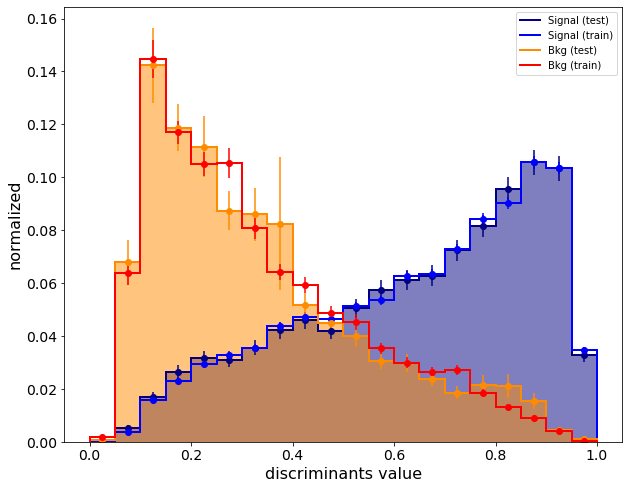
\includegraphics[width=0.8\textwidth]{plots/evtbdt/evtbdt_dist.png} 
    \caption{As an example, the discriminant distributions for the event-level BDT for signal and background in training and validation samples for 2018.}
    \label{fig:evtbdt_dist} 
\end{figure}

\begin{figure}[h!]
    \centering
    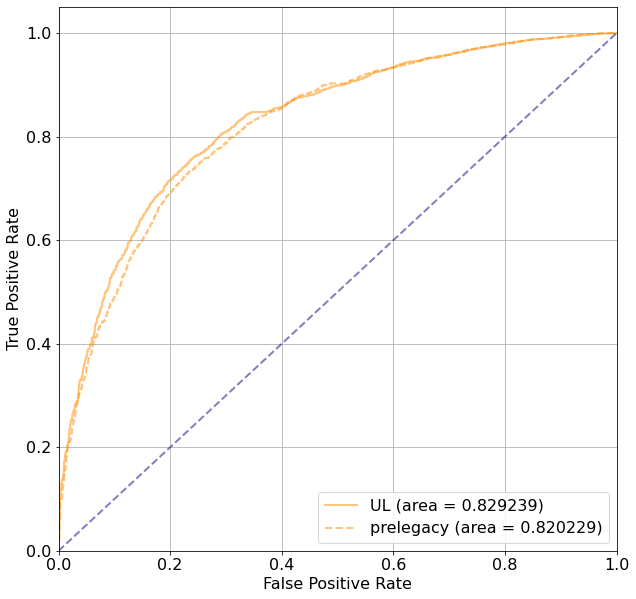
\includegraphics[width=0.8\textwidth]{plots/evtbdt/evtbdt_roc.png} 
    \caption{ROC curves of the event-level BDT for 2018, as compared against the prelegacy model.}
    \label{fig:evtbdt_roc} 
\end{figure}

\section{Background Estimation}
QCD multijet and hadronic $t\bar{t}$ processes are the dominant background of this analysis. Next-to-leading order (NLO) calculations in strong interactions and limited statistics lead to large uncertainties in the simulation of the very high jet and b-jet multiplicity regions of these processes used in this analysis. Therefore, we cannot rely on the simulation-based approach to predict the QCD multijet and $t\bar{t}$ +jets background. To overcome this, we adopt two data-driven methods: the ``extended ABCD " method for data-driven estimation of the absolute rate of the background, and the ``ABCDnn" method for data-driven estimation of the shape of the background.\\

\subsection{Extended ABCD method}
We divide the phase space into two dimensions using $N_j$, the number of jets, and $N_b$, the number of b-jets. In the vanilla ABCD method, the phase space is divided into four regions along the two dimensions, one of which is the Signal Region (SR) D and the other three are Control Regions (CR) A, B and C. The yield in the Signal region D is estimated as $\hat{F}_D = \frac{F_B}{F_A} \times F_C$, where $\hat{F}_D$ is the estimated yield in Signal Region D and $F_A$, $F_B$ and $F_C$ are the observed yield in Control Regions A, B and C respectively. This method assumes joint distributions in $N_j$ and $N_b$ are mostly factorizable.\\

To improve the accuracy of the estimation, we extend the CRs to lower multiplicity in $N_j$ as seen in fig \ref{fig:extendedabcd}. Then, yield in the SR can be estimated as $\hat{F}_D = \left( \frac{F_B F_C}{F_A} \right)^2 \left( \frac{F_X}{F_B F_Y} \right)$.\\ Here, $F$ is the estimated $t\bar{t}$ + QCD multijet yield in each Control Region. This is estimated by subtracting the $t\bar{t}t\bar{t}$ MC yield and minor background processes MC yield from the observed yield in data in each Control Region.\\

The extended ABCD method is applied to each $h_T$ bin as specified in table \ref{tab:sm_sr_definition} for each year separately.\\

Closure test conducted on prelegacy 2016 $t\bar{t}$ events requiring 0 lepton and same regions defined on $N_j$ and $N_b$ shows that yield predicted by vanilla ABCD method if off by 18\%. The disagreement between the estimated and true yield improves to 7\% for the extended ABCD method.\\

Appendix \ref{sec:extendedabcdapp} includes yields for control regions and estimated yield for the signal region for each $H_T$ bin and for each year.

\begin{figure}[ht]
    \centering
    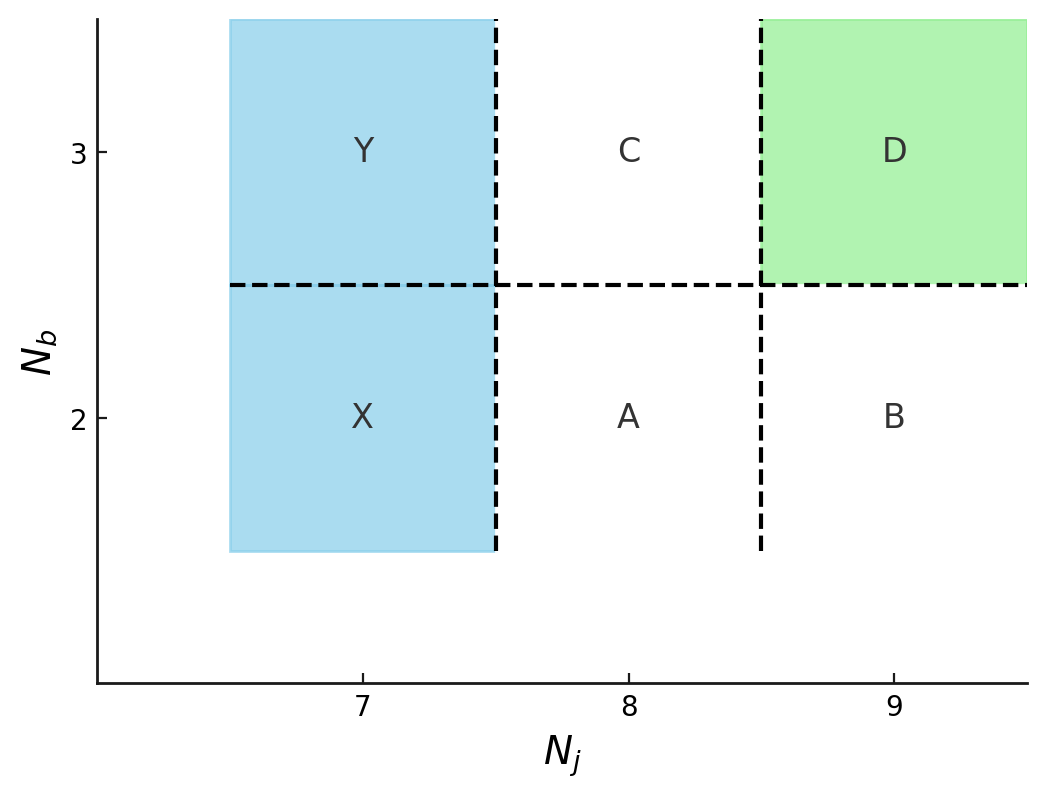
\includegraphics[width=0.8\textwidth]{plots/extendedabcd/extendedabcd_scheme.png} 
    \caption{A, B and C are the Control Regions for the vanilla ABCD method and Y and X are the added adjacent Control Regions for the extended ABCD method. D is the Signal Region}
    \label{fig:extendedabcd} 
\end{figure}

\subsection{ABCDnn method}
We use the ``ABCDnn" method to estimate the shape of the event-level BDT discriminant for the $t\bar{t}$ + QCD multijet background in the Signal Region. Specifically, ``ABCDnn" method utilizes a Machine Learning technique named Neural Autoregressive Flow, which creates transformations between distributions of the feature variables under different conditions. These transformations are constructed as invertible bijective functions implemented as DNNs and learnt during training. In addition, the method automatically take into account the complex correlations between feature variables, so that multi-dimensional distributions can also be estimated. \\

Specifically, for this analysis, we use the same definition of Control Regions and Signal Regions as the ones defined for extended ABCD. That is, the neural networks are trained on Control Regions and applied to the Signal Region. For each Control Region, the neural network takes two distributions for training: the normalized distribution of $t\bar{t}$ MC as the input distribution, and the normalized data-driven estimated $t\bar{t}$ + QCD multijet distribution as the target distribution. The target distribution is created by taking the actual observed data distribution and subtract it by the $t\bar{t}t\bar{t}$ MC distribution and other minor background MC distributions. The neural network learns the transformation from the input distribution to the target distribution in each Control Region, as well as the condition, i.e. the label of the Control Region in the phase space, so that it learns how the transformation should change across the phase space defined by $N_j$ and $N_b$. It does this by minimizing the maximum-mean-discrepancy between the output predicted distribution and the target distribution. Finally, the neural network is applied to the input distribution of $t\bar{t}$ MC in the Signal Region to obtain the desired shape of data-driven estimated $t\bar{t}$ + QCD multijet distribution in the Signal Region.\\

The  learned models in this analysis not only transforms from MC distribution to data-driven distribution to compensate for potential data-MC disagreement, but also transforms from a single process distribution ($t\bar{t}$) to dual process ($t\bar{t}$ + QCD multijet distribution). We do not use the MC QCD multijet distribution as input due to limited statistics, especially in the Signal Region.\\

This training is done for each top-tag instead of each $H_T$ bin because of the limited statistics in each $H_T$ bin. Therefore, for this analysis the feature variables underlying the transformed distributions are event-level BDT discriminant and $H_T$. The predicted $H_T$ of each event in the input distribution is used to place them in the corresponding $H_T$ bin, and the BDT discriminant is used in each $H_T$ bin to create the predicted shape. A separate ``ABCDnn"" model is trained for each year.\\

A closure test for the method has been done by the previous iteration of this analysis morphing $t\bar{t}$ MC distribution into $t\bar{t}X$ MC distributions, with the same event selection and Control/Signal Region definition as the main analysis. The method was found to predict the target shape well.\\

\subsection{Validation of the background estimation methods}
\label{sec:validationregion}
The two background estimation methods are validated in a validation region (VR) requiring lower $N_j$ than the previously defined SR. Specifically, we use $N_j=8, N_b>=3$ as the VR, and define the Control Regions for this VR correspondingly. We then perform the same procedures as defined previously for ``extendedABCD" and ``ABCDnn"", and compare the predicted yield and shape with the truth. \\

We find that the estimated yield in the Validation Region in each $H_T$ bin agrees with the true yield after accounting for statistical error from MC propagated through the extended ABCD formula and statistical error in the true yield. The result is in Appendix \ref{sec:extendedabcdvalapp}. We account for the disagreement as a systematic uncertainty detailed in section \ref{sec:systextendedabcd}.\\

We find that the predicted shape in the Validation Region largely agrees well with the true shape, especially for $H_T$ bins with higher statistics. The result is in Appendix \ref{sec:abcdnnvalapp}. We account for the disagreement as a systematic uncertainty detailed in section \ref{sec:systabcdnn}. 



\section{Systematic uncertainties}
\label{sec:syst}
\subsection{Systematics from background estimation}
We derive the systematic uncertainties for our background estimation methods from the Validation Region defined in section \ref{sec:validationregion}, where we compare the output (yield/shape) of the specific background estimation method against the truth. We then apply the derived systematics to the Signal Region. These uncertainties are calculated separately for each $H_T$ bin defined in table \ref{tab:sm_sr_definition}.

\subsubsection{ExtendedABCD}
\label{sec:systextendedabcd}
We derive a normalization uncertainty from the Validation Region based on the disagreement between the data and predicted background in the VRs. This uncertainty is calculated in each VR $H_T$ bin as the sum in quadrature of two quantities: the deviation of the weighted mean (average) of events in that VR $H_T$ bin from 1, and the weighted RMS of events in that VR $H_T$ bin. The weighted mean $\langle f \rangle$ is defined as 
\[
\langle f \rangle = \frac{\sum_i f_i w_i}{\sum_i w_i},
\]
for each discriminant histogram bin $i$ in the VR $H_T$ bin of interest, where the weight $w_i$ is the number of events in that histogram bin and $f_i$ is the ratio of observed events to predicted events ($N_{\text{data}} / N_{\text{pred}}$) in that histogram bin. The mean is weighted to reflect the distribution of events in the histogram, and the deviation of this weighted mean from 1, i.e. $(1 - \langle f \rangle)$ reflects the overall offset in normalization between the prediction and the data. Similarly, the weighted RMS is defined as 
\[
\sqrt{\langle f^2 \rangle - \langle f \rangle^2},
\]
where
\[
\langle f^2 \rangle = \frac{\sum_i f^2_i w_i}{\sum_i w_i},
\]
and reflects the spread of the disagreement between the prediction and the data in the histogram bins. This method of quantifying the data-prediction discrepancy is based on recommendations from the CMS Statistics Committee. These uncertainties are taken to be uncorrelated across $H_T$ bins and years.

\subsubsection{ABCDnn}
\label{sec:systabcdnn}
We derive an uncertainty for the shape of ABCDnn output from the Validation Region, based on observed disagreement between the shape of data and predicted background in the VRs. This uncertainty is calculated in each VR $H_T$ bin as a linear shift, both up and down, of the BDT discriminant value of each event. For example, a shift up of 2\% ($s=+0.02$) for a particular VR $H_T$ bin means that the BDT discriminant value of every event in that VR $H_T$ bin is multiplied by 1.02. Qualitatively, in both up and down directions, we shift the BDT discriminants such that the disagreement between the shape of the normalized BDT discriminant distribution of the data and the predicted background is as small as possible. Quantitatively, the extent of the shift is determined by minimizing the following metric:

\[
s = \arg\min_s \sum_i \max\left(\frac{|f_i(s) - 1|}{\sigma_i(s)}, \frac{|f_i(0.0) - 1|}{\sigma_i(0.0)}\right)
\]

where s is a particular shift up (positive) or down (negative), $f_i = \frac{N_{\text{pred}, i}}{N_{\text{truth}, i}}$, the ratio of predicted events over observed events in BDT discriminant bin i, and $\sigma_i$ is the statistical uncertainty in bin i. $\frac{|f_i(s) - 1|}{\sigma_i(s)}$ measures the deviation of ratio in bin i from 1 under shift s, inversely scaled by the statistical uncertainty in that bin. In most cases, the deviation increases for some bins and decreases for the others under a particular shift, therefore a naive minimization of this term across the bins results in bad coverage in the bins whose deviation decreases. These bins are the bins that are supposed to be covered by the shift, since the bins whose deviation increases would be covered by the shift in the opposite direction.\\ 

To overcome this, we include a maximization against the second term
$\frac{|f_i(0.0) - 1|}{\sigma_i(0.0)}$, which is the same scaled deviation of ratio before shifting. The maximization of the first term against the unshifted scaled deviation of ratio removes the effect of bins whose deviation worsened under a particular shift direction, so that by minimizing this metric, the shifting method can obtain good coverage of disagreement in all bins.\\

Currently, we consider this shape uncertainty as uncorrelated across $H_T$ bins and across years.



\subsubsection{Closure Test on systematic uncertainty estimation for background estimation}

We perform closure tests to make sure that the methods used to estimate the systematic uncertainties of the two background estimation are reasonable. We use ultralegacy 2018 data, using exactly the same requirement as our event selection and inputs to extended ABCD formula, and using the same $H_T$ bin definition as $N_RT$=1, $N_BT$=0 top-tag, but requiring 0 resolved top instead of at least 1 so that the regions are orthogonal from the main analysis. In this region, we estimate the systematic uncertainties of the two background estimation methods in the VR, and apply them to the SR, and finally compare the predicted yield and shape with the truth in SR while taking into account the estimated systematic uncertainties.\\

For ``extendedABCD", the result shows that the estimated yield in the Signal Region in each $H_T$ bin agrees with the true yield after accounting for statistical error from MC propagated through the extended ABCD formula and statistical error in the true yield, as well as the systematic uncertainty as defined in sec \ref{sec:systextendedabcd}. The result is in Appendix \ref{sec:extendedabcdclosuretestapp}.\\

For ``ABCDnn", the result shows that the systematic uncertainty as defined in sec \ref{sec:systabcdnn} mostly covers the disagreement between the predicted and the true shape in each $H_T$ bin in the Closure Test region. The result is in Appendix \ref{sec:abcdnnclosuretestapp}.\\

\subsection{Other sources of systematic uncertainties}


\begin{itemize}
    \item The statistical uncertainties of SM/top philippic $t\bar{t}t\bar{t}$ signal samples and background processes modeled with MC samples.
    \item The statistical uncertainties of the estimated QCD + $t\bar{t}$ yields in each CR, propagated through the extendedABCD formula.
    \item The statistical uncertainties of the simulated $t\bar{t}$ events transformed by ABCDnn to form the predicted discriminant distribution of BDT.
    \item The statistical uncertainties from the trigger efficiency corrections, parameterized in $N_b$ and $N_j$.
    \item Uncertainties related to the boosted top and W tagging correction factors used to correct the performance of the Particlenet algorithm in simulation to match data. Two uncertainties are included: boosted top and boosted W uncertainties related to the non-mass-decorrelated scale factors. These uncertainties are correlated between processes but uncorrelated between years.
    \item Tagging and misidentification uncertainties related to resolved top tagging correction factors used to correct the performance of the resolved top tagging algorithm in simulation to match data, as described in Section \ref{sec:restop}. Two uncertainties for both tagging efficiency and mistag rate scale factors are considered, and uncertainties in these stem from statistical uncertainties that arise in calculating the scale factors. These are correlated between processes and uncorrelated between years.
    \item Uncertainties related to correction factors used to correct for the performance of the DeepJet b-tagging algorithm in simulation with respect to data. The DeepJet iterative fit/shape scale factors are used. Scale factors per event are calculated as the  product of the scale factors for all jets in a given event passing pre-selection. The uncertainties are split into several sources, including those affecting HF (heavy-flavor) or LF (light-flavor) jets, uncertainties from charm jets (cferr1 and cferr2), and linear and quadratic statistical fluctuations (LFstats1, LFstats2, HFstats1, HFstats2). These are all considered as separate systematic variations, with statistical variations correlated between processes and uncorrelated between years (LFstats1, LFstats2, HFstats1, HFstats2) and others correlated between both processes and years (HF, LF, cferr1 and cferr2).
    \item Uncertainties associated to the pileup reweighting correction factor.
    \item Jet energy scale (JES) and resolution (JER) uncertainties impacting the reconstruction of jets, including R = 0.4 and R = 0.8 jets, $p_T^{miss}$ , and tagged top, W, and b candidates and their correction factors. The JES systematic uncertainty is currently applied using the combined JES uncertainty. We vary the JES and JER up and down by their systematic uncertainties and propagate the effects through all analysis objects and selections, including in selecting jets and boosted objects and re-propagating the varied jets through our resolved top algorithm. JER and JES variations are correlated between processes but not between years.
    \item Uncertainties assigned to the integrated luminosity measured by the CMS experiment.
    \item Uncertainties in the theoretical cross sections used to normalize ttX backgrounds are considered. These impact the number of ttX events in each SR bin. For ttX processes (X=W,Z,H), we assign an uncertainty of 26\% based on the largest deviation of the signal strength observed by CMS for any of these processes (relative to the SM prediction).
    
\end{itemize}

\section{Results and interpretation}
A binned likelihood analysis is carried out in the SR categories split by resolved and boosted top multiplicities and $H_T$, as defined in Table \ref{tab:sm_sr_definition}. As input to each SR category, the shape and yields of the event-level BDT discriminant of $t\bar{t}t\bar{t}$, $t\bar{t}X$ and other minor background processes are provided to CMSCombine from Monte Carlo, and those of $t\bar{t}$ and QCD processes are provided from data-driven background estimation methods extendedABCD (Section \ref{sec:systextendedabcd}) and ABCDnn (Section \ref{sec:systabcdnn}). \\

The systematic uncertainties described in Section \ref{sec:syst} are included in the analysis as nuisance parameters. Up and down variations of the BDT discriminant shapes are provided as inputs for each nuisance parameter corresponding to shape-based systematic variations, while uncertainties affecting only the normalizations of processes are implemented using log-normally distributed constraints on the simulation rates in each data-taking period.\\

Currently at the blinded stage, we have the following preliminary result:\\

\begin{table}[h!]
    \centering
    \begin{tabular}{lcc}
        \toprule
        & \textbf{Expected significance} & \textbf{Median expected limit} \\
        \midrule
        2016 + 2016preVFP & 0.753 & 3.281 \\
        2017              & 0.669 & 4.813 \\
        2018              & 0.493 & 5.281 \\
        2022 + 2022EE     & 0.753 & 3.688 \\
        \midrule
        \textbf{Total}    & \textbf{1.441} & \textbf{1.500} \\
        \bottomrule
    \end{tabular}
    \caption{Expected significance and median expected limits for SM $T\bar{T}T\bar{T}$.}
    \label{tab:combine_res_blineded_sm}
\end{table}

\begin{table}[h!]
    \centering
    \begin{tabular}{l c c c}
        \toprule
        \textbf{$M_{v_{1}}$ / GeV} & \textbf{$c_t$} & \textbf{Expected significance} & \textbf{Median expected limit} \\
        \midrule
        \multirow{3}{*}{1400} & 3.0 & 0.928 & 2.289 \\
                              & 2.5 & 0.700 & 3.047 \\
                              & 2.0 & 0.446 & 4.813 \\
        \midrule
        \multirow{3}{*}{1200} & 3.0 & 1.838 & 1.129 \\
                              & 2.5 & 1.330 & 1.578 \\
                              & 2.0 & 0.947 & 2.242 \\
        \midrule
        \multirow{3}{*}{1000} & 3.0 & 3.594 & \textbf{0.561} \\
                              & 2.5 & 2.744 & \textbf{0.746} \\
                              & 2.0 & 2.001 & 1.039 \\
        \midrule
        \multirow{3}{*}{800}  & 2.5 & 5.444 & \textbf{0.361} \\
                              & 2.0 & 3.965 & \textbf{0.506} \\
                              & 1.5 & 2.586 & \textbf{0.793} \\
        \midrule
        \multirow{3}{*}{600}  & 2.5 & 10.062 & \textbf{0.192} \\
                              & 2.0 & 7.471  & \textbf{0.259} \\
                              & 1.5 & 5.013  & \textbf{0.393} \\
        \bottomrule
    \end{tabular}
    \caption{Expected significance and median expected limits for various $M_{v_{1}}$ and $c_t$ values for the top-philic BSM model for 2018.}
    \label{tab:combine_res_top_philic}
\end{table}

\appendix
\section{Control Region Distributions}
\section{Resolved top tagger SF distributions}
\section{Event-level BDT distributions}
\section{Extended ABCD yields}
\label{sec:extendedabcdapp}
\section{Extended ABCD validation}
\label{sec:extendedabcdvalapp}
\section{ABCDnn predicted shape}
\label{sec:abcdnnapp}
\section{ABCDnn validation}
\label{sec:abcdnnvalapp}
\section{Extended ABCD closure test}
\label{sec:extendedabcdclosuretestapp}
\section{ABCDnn closure test}
\label{sec:abcdnnclosuretestapp}

\bibliographystyle{plain}
\bibliography{references}
\end{document}
